\documentclass[12pt,a4paper]{book}
\usepackage[utf8]{inputenc}
\usepackage[spanish]{babel}
\usepackage{amsmath}
\usepackage{multirow, array} % para las tablas
\usepackage{float}
\usepackage{amsfonts}
\usepackage{amssymb}
\usepackage{graphicx}
\usepackage{enumerate} % enumerados
\usepackage[left=2cm,right=2cm,top=2cm,bottom=2cm]{geometry}
\usepackage{pdfpages}
\usepackage{subfigure}
\usepackage{verbatim}%comentarios
\usepackage[T1,hyphens]{url}
\usepackage{appendix}


\usepackage[breaklinks=true]{hyperref}
\usepackage{booktabs}

\setcounter{secnumdepth}{3} %para que ponga 1.1.1.1 en subsubsecciones
\setcounter{tocdepth}{3} % para que ponga subsubsecciones en el indice
\hypersetup{pdfborder={0 0 0}}


\begin{document}
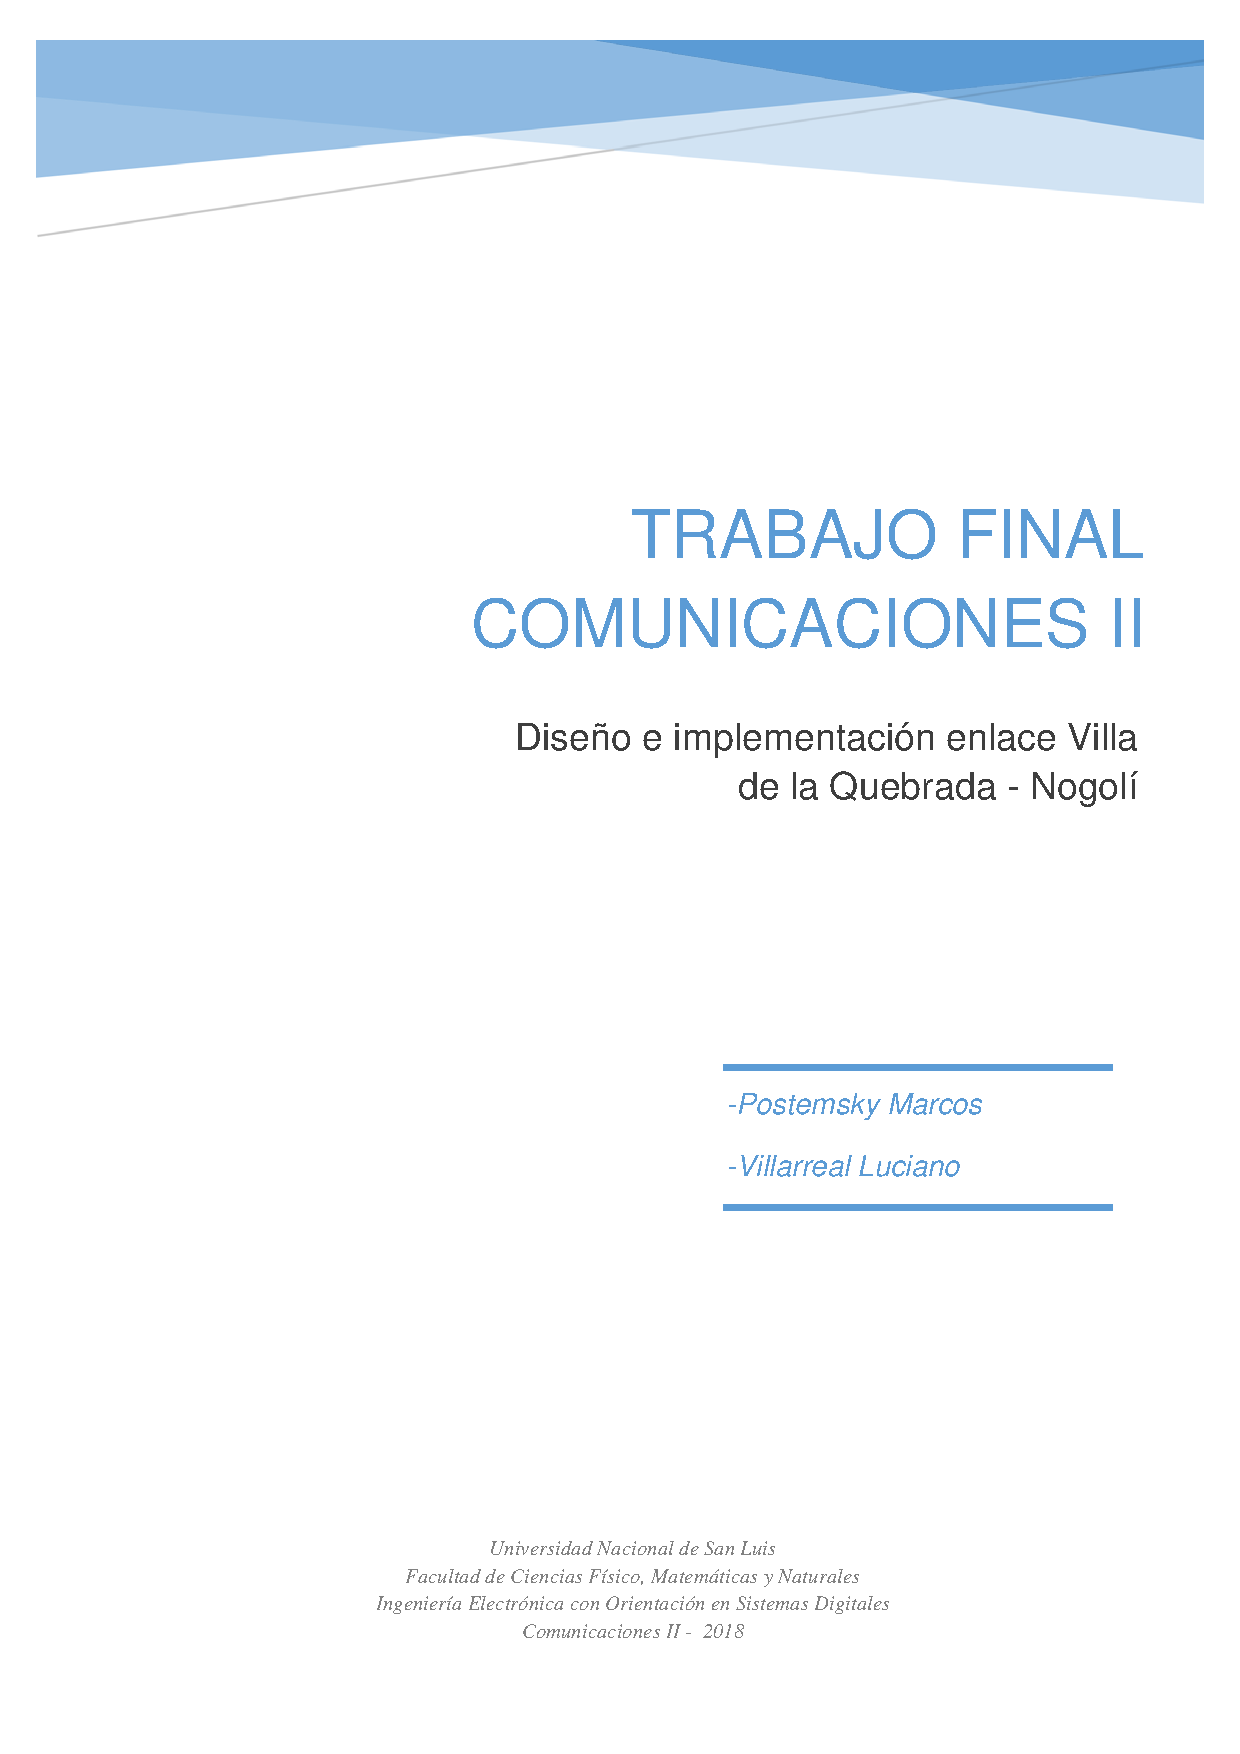
\includepdf{../figuras/portada.pdf}

 %para crear una cara en blanco
$\ $

\pagenumbering{Roman} % para comenzar la numeración de paginas en números romanos
\tableofcontents % indice de contenidos

\renewcommand{\tablename}{Tabla}
\renewcommand{\figurename}{Fig.}

\renewcommand{\appendixname}{Anexos}
\renewcommand{\appendixtocname}{Anexos}
\renewcommand{\appendixpagename}{Anexos}

\listoffigures % indice de figuras

\listoftables % indice de tablas 


\chapter{Introducción}
\pagenumbering{arabic}

En el presente documento se plantea el diseño de una red de telecomunicaciones con el objetivo de brindar servicio triple play en la localidad de Nogolí, San Luis, Argentina; abordando el estudio desde el punto de vista técnico, demográfico, social y económico. 

Para la conformación del mismo se han realizado estudios demográficos y socio-económicos, capitulo 4 "Análisis demógrafico y socio-economico", con la finalidad de determinar la capacidad de la red así como la factibilidad del proyecto.

En el capítulo 5 "Red de transporte" del presente documento, se realiza un análisis técnico y económico del enlace punto a punto (en adelante, "enlace PaP") requerido para la red de transporte, donde se plantea su implementación con fibra óptica o radioenlace. 

Una vez definida la red de transporte, se realiza el mismo análisis para el diseño e implementación de la red de acceso (Capítulo 6 "Red de acceso") determinando, con base en estudios económicos y técnicos, la topología a utilizar así como el medio de transmisión. 

El documento concluye con el desarrollo de un plan de negocios (Capítulo 8 "Plan de negocios"), donde se detalla la viabilidad del proyecto en su totalidad, así como los requerimientos y proyecciones en materia económica a corto y largo plazo.


\chapter{Objetivos}\label{objetivos}

Este trabajo final tiene como objetivo realizar un análisis y planeamiento profesional para brindar el servicio Triple Play a la Localidad de Nogolí, realizando la conexión desde la localidad de Villa de la Quebrada, ambas de la provincia de San Luis.  Mediante los conocimientos adquiridos en el curso de Comunicaciones II, se deberá realizar un análisis de pre-ingeniería, ingeniería y de factibilidad económica y técnica sobre la conexión de la localidad mencionada. A continuación, se hace mención de los objetivos principales del trabajo integrador:

\begin{itemize}
\item Desarrollo de un análisis de pre-ingeniería, ingeniería y factibilidad dirigido a la prestación de Servicio triple play (Internet, TV y voz).
\item Mejorar la capacidad de los integrantes del grupo en la toma y justificación de decisiones.
\item Visualizar y entender los pasos a seguir en el inicio y proceso de una obra.
\item Tener en cuenta las normas vigentes y donde encontrarlas.
\item Asesoramiento con terceros.
\item Practicar el trabajo en equipo, muy importante para el mundo profesional.
\end{itemize}

No solo se aplicarán conceptos relacionados a la materia Comunicaciones II, ya que la amplitud del trabajo permite abarcar temas que engloban a la carrera de Ingeniería Electrónica con O.S.D, como así también temas de contabilidad y gestión. Es necesario resaltar que se debe concluir el trabajo determinando la viabilidad del proyecto a 3 o más años.


\chapter{Análisis demográfico y socio-económico}\label{cap_demografico}

Para determinar la capacidad de datos necesaria para la distribución del servicio triple play en la localidad de Nogolí, provincia de San Luis, se analizan de diferentes fuentes (principalmente estadísticas del INDEC y la Dirección Provincial de Estadísticas y Censos de San Luis) las estadísticas poblacionales del departamento Belgrano, como así también de Nogolí. 

A continuación, se presenta toda la información utilizada para determinar la penetración del servicio y modelos de consumo requeridos para obtener la capacidad de datos necesaria. Se debe tener en cuenta que gran parte de la información obtenida hace referencia a las estadísticas de todo el departamento Belgrano, por lo cual con ayuda de proyecciones y la relación localidad/departamento, se utiliza dicha información para representar las estadísticas de la localidad de Nogolí.

\section{Población urbana y rural}

Se define como población urbana aquella que habita en una localidad de 2000 o más habitantes; y población rural aquella que se encuentra agrupada en localidades de menos de 2000 habitantes o dispersa en campo abierto. En la provincia de San Luis la población rural ha ido disminuyendo como consecuencia del proceso de urbanización.

Del total de la población rural, durante los últimos tres censos, el porcentaje de población en localidades con menos de 2000 habitantes (rural agrupada) ha ido creciendo, mientras que la población en áreas rurales dispersas ha ido disminuyendo.

Los dos departamentos con población netamente rural han sido San Martín y Belgrano, donde Belgrano presenta el mayor porcentaje de población rural agrupada.

\begin{figure} [H]
\centering
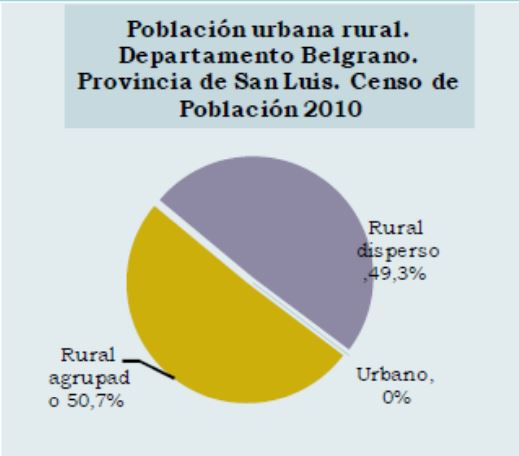
\includegraphics[width= 6cm]{../figuras/4_1_Fig1.jpg}
\caption{Población urbana-rural. Departamento Belgrano. Censo 2010. Fuente: Dirección Provincial de Estadísticas y Censos de San Luis}
\label{fig_pob_urbRur_dem}
\end{figure}	


En Fig. \ref{fig_evolucion_dem}, se presenta una gráfica de la evolución demográfica de Nogolí, entre 1980 y 2010. En dicha gráfica, es posible notar el crecimiento constante que ha tenido Nogolí en 30 años, por lo cual se considera que dentro de 10 años la población seguirá creciendo, no solo por lo que demuestran las estadísticas, sino también, las conocidas inversiones que se han realizado en el transcurso de los años en la localidad de Nogolí; un gran ejemplo es el dique al pie de las Sierras de San Luis, y la ruta que conecta Nogolí con Río grande que en su punto más alto supera los 1900 metros, siendo una gran atracción turística.

\begin{figure} [H]
\centering
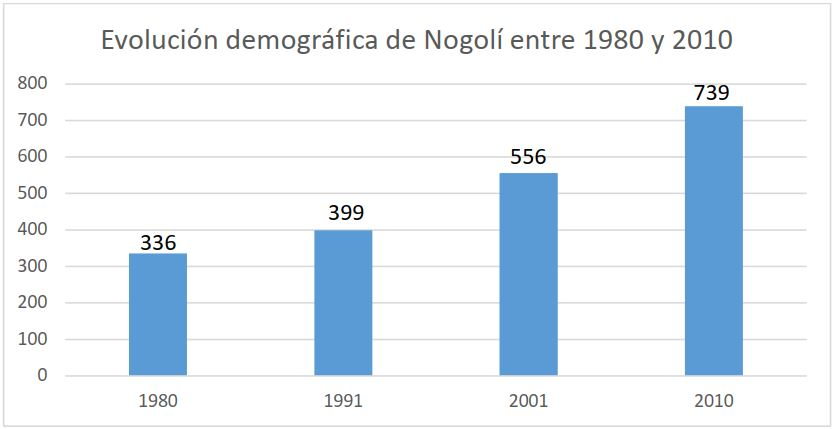
\includegraphics[width= 15cm]{../figuras/4_1_Fig2.jpg}
\caption{Gráfica de evolución demográfica de Nogolí.}
\label{fig_evolucion_dem}
\end{figure}	

Previo a comentar las proyecciones de la población a diez años, se considera importante para la distribución del servicio triple play, no solo la cantidad de hogares establecidos en Nogolí sino también el promedio de personas por hogar en la localidad.

Si notamos que el promedio de personas por hogar se mantiene desde el 2001 al 2010, es posible utilizar esta información para el año 2020 con su respectiva proyección en población.

En 2001 en el Departamento Belgrano se censaron 3881 personas en 1192 hogares. Luego, en el año 2010, también en el Departamento Belgrano, se censaron 3945 personas en 1294 hogares. Por último, según el censo de 2001 en Nogolí, se censaron 558 personas en 174 hogares. En Tabla \ref{tab_est_hog_dem} se exponen los datos antes mencionados.

\begin{table}
\centering
\begin{tabular}{|c|c|c|c|c|c|}
\hline 
Año & Dpto/Localidad & Población & Hogares & Personas/hogar & \%Hogares con NBI \\ 
\hline 
2001 & Belgrano & 3881 & 1192 & 3.26 & 37.6\% \\ 
\hline 
2010 & Belgrano & 3945 & 1294 & 3.05 & 22.6\% \\ 
\hline 
2001 & Nogolí & 558 & 174 & 3.19 & - \\ 
\hline 
\end{tabular} 
\caption{Estadísticas de hogares en Belgrano/Nogolí.}
\label{tab_est_hog_dem}
\end{table}



En Fig. \ref{fig_evolucion_dpto_dem} se presenta un gráfico que corresponde a la evolución demográfica del departamento de Belgrano entre los años 1980 y 2010, el cual se usará luego para proyectar la población de Nogolí.

\begin{figure} [H]
\centering
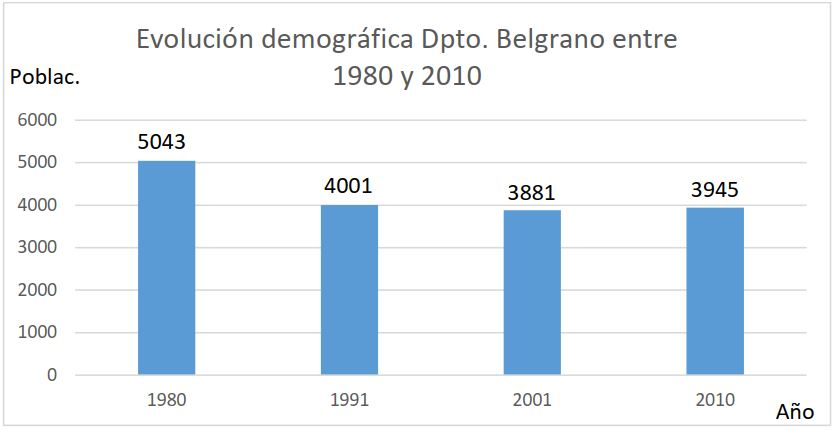
\includegraphics[width= 10cm]{../figuras/4_1_Fig3.jpg}
\caption{Gráfica de evolución demográfica del Dpto. Belgrano. (Fuente: INDEC)}
\label{fig_evolucion_dpto_dem}
\end{figure}	


Comparando los gráficos de Fig. \ref{fig_evolucion_dem} y Fig. \ref{fig_evolucion_dpto_dem}, es notable la diferencia entre la evolución demográfica de Nogolí respecto al Dpto. Belgrano, aunque es algo esperado por lo comentado anteriormente.

En el año 2001 Nogolí representaba el 14.3 \% de la población en el departamento. Luego, en el año 2010 Nogolí representaba el 18.7\%, indicando que entre esos años, la población en Nogolí ha aumentado. Este aumento puede deberse a una redistribución de habitantes en el departamento, ya que el crecimiento neto ha sido casi nulo.

Téngase en cuenta que Nogolí en 10 años creció un 33\%, algo no muy común en el comportamiento de la población. En Fig. 4.1.4, se muestra una proyección de la población hasta el año 2025 de la localidad de Nogolí, dicha proyección fue realiza por INDEC para el departamento Belgrano pero teniendo en cuenta que Nogolí representa del 18\% al 20\% de la población del departamento se obtiene el gráfico antes mencionado.


\begin{figure} [H]
\centering
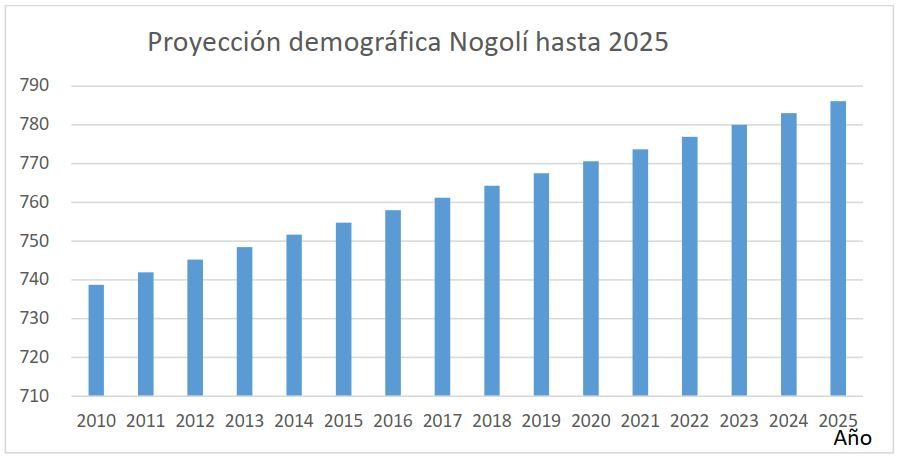
\includegraphics[width= 12cm]{../figuras/4_1_Fig4.jpg}
\caption{Proyección demográfica de Nogolí hasta el año 2025. (Fuente: INDEC)}
\label{fig_proy_25_dem}
\end{figure}

Puede verse en Fig. \ref{fig_proy_25_dem} que la proyección es conservadora respecto al crecimiento notable que se encuentra en Fig. \ref{fig_evolucion_dem}, pero teniendo en cuenta que la tasa de datos necesaria para el enlace será calculada para dejar un margen de crecimiento, se considera como buena práctica ser conservadores.

Para el año 2018 la proyección predice una población de 764 personas en la localidad de Nogolí, lo que totaliza 243 hogares (teniendo en cuenta el promedio de 3.15 personas por hogar de la Tabla \ref{tab_est_hog_dem}), de los cuales un 22.6 \% son hogares con NBI (Necesidades Básicas Insatisfechas) considerando las estadísticas del 2010, aunque este tendía a reducirse.

Para el año 2025 la proyección predice una población de 786 personas en la localidad de Nogolí, como el promedio de 3.15 personas por casas se mantuvo desde el año 2001, teniendo en 2010 un crecimiento del 33\%, se sigue considerando dicho promedio, por lo cual se tendrían unos 250 hogares para el año 2025.

Como conclusión para este año 2018, descontado los hogares con NBI (aproximadamente 55 viviendas), son 188 los abonados potenciales para la distribución de tripleplay en Nogolí. Dado que en la localidad de Nogolí no se ofrece servicio triple play por parte del sector privado, más adelante se profundiza en el tema, se plantea como objetivo cubrir el 60\% del mercado, es decir 113 hogares. Con base en estudios y encuestas realizadas, se considera que el porcentaje propuesto es conservador (no es conveniente diseñar el proyecto basado en suposiciones demasiado ambiciosas, como lo sería considerar el 100\% del mercado) y con una posibilidad alta de éxito.


\section{Análisis Socioeconómico} \label{sec_analisis_socieconomico}

Con base en el documento “Salarios y puestos de trabajo del sector privado registrado 2016” \footnote{Fuente: Dirección Provincial de Estadística y Censos, Secretaria General de la Gobernación, Gobierno de la Provincia de San Luis}, es posible proyectar la remuneración neta promedio de los puestos de trabajo privados para el 2018 teniendo en cuenta la inflación y las paritarias salariales propuestas hasta el día de la fecha. Cabe destacar que la proyección es una estimación del posible valor de la remuneración a futuro, y estas pueden diferir a las calculadas. Aún así, con una estimación de la economía del ciudadano se puede predecir a grandes rasgos el posible precio del servicio, teniendo en cuenta la competencia y otros factores que se discuten más adelante.


\begin{figure} [H]
\centering
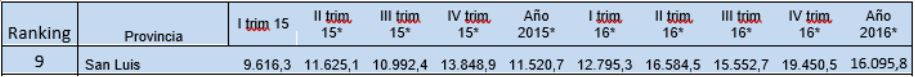
\includegraphics[width= 15cm]{../figuras/4_2_Fig1.jpg}
\caption{Remuneración promedio. (Fuente: Dirección Provincial de Estadística y Censos, Secretaria General de la Gobernación, Gobierno de la Provincia de San Luis)}
\label{fig_rem_prom}
\end{figure}


En Fig. \ref{fig_rem_prom} se expone la remuneración neta para los cuatro trimestres del año 2015 y 2016. Siendo el promedio en 2015 de \$11520 y en 2016 de \$16095. Se observa que hubo un aumento del 39.71\%. Teniendo en cuenta que la inflación anual en 2017 fue del 24.6\% aproximadamente (Fuente: Infobae), si se supone un aumento del poder adquisitivo a la par de la inflación (supongamos 20\%) se puede estimar una remuneración neta promedio de \$19.314 en 2017. Para el 2018 se prevé un aumento salarial del 15\% en promedio para diversos sectores \footnote{Fuente: https://www.portaldeltrabajador.com.ar/paritarias visitada el 17/09/2018}, se puede estimar a grandes rasgos una remuneración de \$22211 promedio para el 2018. Los cálculos realizados son una aproximación para tener una idea global de la remuneración promedio de los habitantes y a partir de allí poder estimar los precios de los servicios que se brindarán.



\chapter{Análisis de mercado} \label{sec_analisis_mercado}

En la localidad de Nogolí no se brinda servicio de triple play por parte del sector privado. La ciudadanía dispone de la red de WI-FI gratuito brindado por Autopista de la Información y según fuentes locales, se tiene acceso sólo a telefonía móvil GSM y TV satelital.

Se ha detectado que la localidad dispone de 7 antenas WI-FI a 2.4 GHz con un promedio de 46 usuarios por antena, lo que indica una baja tasa de datos por usuario.

Considerando los datos antes mencionados se justifica el hecho de brindar servicio triple play en Nogolí, dada la alta demanda y casi nula oferta.

\section{Servicios propuestos}

\begin{table}[H]
\centering
\begin{tabular}{|c|>{\centering}m{6cm}|c|c|}
\hline 
\textbf{Servicio} & \textbf{Tv Digital} & \textbf{Internet} & \textbf{VoIP} \\ 
\hline 
\textbf{Paquete 1 (Básico)} & SDTV (50 canales estándar) & Hasta 4Mbps & 30Kbps \\ 
\hline 
\textbf{Paquetes 2 (Premium)} & SDTV (50 canales estándar)+ HDTV (20 canales HD) & Hasta 6Mbps & 30Kbps \\ 
\hline 
\end{tabular}
\caption{Servicios propuestos}
\label{tab_serv_prop_dem}
\end{table}



\section{Cálculo de capacidades}

Para el cálculo de la capacidad total requerida para la implementación de la red de transporte se detalla la máxima capacidad necesaria para cada servicio por separado, teniendo en cuenta dos aspectos fundamentales; factor de re-uso, que será de 1:7 (es decir que de siete abonados, sólo uno estará consumiendo datos), y el porcentaje de los posibles abonados por paquete. 
Se considera que un 60\% de los abonados contratan el paquete 1 (Básico), y el 40\% restante el paquete 2 (Premium). Por lo tanto, el paquete básico consta con 68 abonados, y el Premium con 45. Dichas suposiciones se basan en datos empíricos obtenidos a partir de encuestas realizadas a los habitantes de la zona.



\subsection{TV Digital}

Para brindar servicio de TV digital, se tiene en cuenta que un canal de definición estándar SDTV requiere una tasa de 1.5 Mbps, mientras que para un canal de alta definición HDTV se necesitan 6 Mbps.

La capacidad requerida para brindar el servicio se calcula con base en la cantidad de televisores destinada para cada paquete. Se establece que el promedio de televisores por hogar en la localidad de Nogolí es de 1.5. Por lo tanto:
\medskip

\noindent\textbf{Paquete 1:}

Servicio destinado a 68 abonados, con un promedio de 1.5 televisores por hogar se obtiene un total de 102 televisores, donde la máxima exigencia se dará cuando todos los televisores se encuentren sintonizando un canal SDTV en simultáneo. Para este caso se tiene que:

\begin{center}

\begin{equation}
CAPACIDAD TV DIGITAL _{PAQUETE 1} = CANTIDAD DE TVs * 1.5 Mbps
\end{equation}

\begin{equation}
CAPACIDAD TV DIGITAL _{PAQUETE 1} = 102 TVs * 1.5 Mbps = 153 Mbps
\end{equation}

\end{center}

\noindent\textbf{Paquete 2:}

Este servicio está destinado para 45 abonados, por lo que se estima un total de 68 televisores. La máxima exigencia se calcula en caso que la totalidad de televisores estén sintonizados en un canal HDTV, en forma simultánea, por lo tanto:

\begin{equation}
CAPACIDAD TV DIGITAL _{PAQUETE 2} = CANTIDAD DE TVs * 6 Mbps
\end{equation}

\begin{equation}
CAPACIDAD TV DIGITAL _{PAQUETE 2} = 68 TVs * 6 Mbps = 408 Mbps
\end{equation}

La capacidad máxima será la suma de las capacidades requeridas por ambos paquetes, por lo tanto se obtiene:

\begin{equation}
CAPACIDAD TV DIGITAL _{MAXIMA} = 153 Mbps + 408 Mbps = 561 Mbps
\end{equation}

Aplicando el factor de re-uso del 14.3\% (1:7), la capacidad máxima necesaria para Tv Digital se reduce a:

\begin{equation}
CAPACIDAD TV DIGITAL _{FINAL} = 561 Mbps * 1/7 = 80.14 Mbps
\end{equation}



\subsection{Internet}

En el presente caso, la capacidad máxima se establece según la cantidad de abonados y el tipo de servicio destinado.
\medskip
\noindent\textbf{Paquete 1:}

El presente servicio ofrece una tasa de datos máxima por abonado de 4 Mbps, por consiguiente:

\begin{equation}
CAPACIDAD INTERNET _{PAQUETE 1} = Cantidad de abonados * 4 Mbps
\end{equation}

\begin{equation}
CAPACIDAD INTERNET _{PAQUETE 1} = 68 * 4 Mbps = 272 Mbps
\end{equation}
\medskip
\noindent\textbf{Paquete 2:}

El presente servicio ofrece una tasa de datos máxima por abonado de 6 Mbps, por consiguiente:

\begin{equation}
CAPACIDAD INTERNET _{PAQUETE 2} = Cantidad de abonados * 6 Mbps
\end{equation}

\begin{equation}
CAPACIDAD INTERNET _{PAQUETE 2} = 45 * 6 Mbps = 270 Mbps
\end{equation}

La capacidad máxima requerida por ambos paquetes es de 542 Mbps. Aplicando el factor de re-uso de 1:7 se concluye que la capacidad requerida para brindar servicio de internet es de 

\begin{equation}
CAPACIDAD INTERNET _{FINAL} = 542 Mbps * 1/7 = 77.42 Mbps
\end{equation}

\subsection{VoIP}

Dado que el servicio de VoIP (Voz sobre IP) requiere una tasa de 30 Kbps, independientemente del paquete adquirido por el cliente, y siendo 113 los potenciales abonados se obtiene:

\begin{equation}
CAPACIDAD VoIP = 113 * 30 Kbps = 3.39 Mbps
\end{equation}

Aplicando el factor de re-uso

\begin{equation}
CAPACIDAD VoIP _{FINAL} = 3.39 Mbps * 1/7 = 0.48 Mbps
\end{equation}

Finalmente, la capacidad necesaria para brindar el servicio completo, ambos paquetes, es la suma de las capacidades antes calculadas:

\begin{equation}
CAPACIDAD NECESARIA _{TOTAL} = [80.14 + 77.42 + 0.48] Mbps  = 158.04 Mbps
\end{equation}

\section{Proyección tasa de datos para el año 2025}

Por último, teniendo en cuenta que en el año 2025 se tendrá un mercado potencial de 200 hogares (sin contar hogares con NBI) y suponiendo que se ocupa un 80\% de dicho mercado, 20\% mayor al mercado ocupado en el caso anterior, resulta un total de 160 hogares. Si se supone que se siguen brindando los dos servicios con la misma proporción y el factor de re-uso sigue siendo del 14.3 \%, se utilizan los cálculos anteriores, para llegar al siguiente resultado:

\begin{equation}
CAPACIDAD NECESARIA TOTAL _{2025} =  222.9 Mbps
\end{equation}



\chapter{Red transporte}

En esta sección, se realizará la selección del medio de transmisión y lo equipos que se utilizarán para la instalación de la red de Transporte, que es la encargada de realizar la comunicación desde la Red de acceso al Núcleo de Red. Recuerde, que en este caso la Red de Acceso se encontrará en la Localidad de Nogolí y el Núcleo de Red (suponiendo que es el proovedor a quién se le comprará el servicio) en la Localidad de Villa de la Quebrada. En la Fig. \ref{fig_jerarquia_redes}.

\begin{figure} [H]
\centering
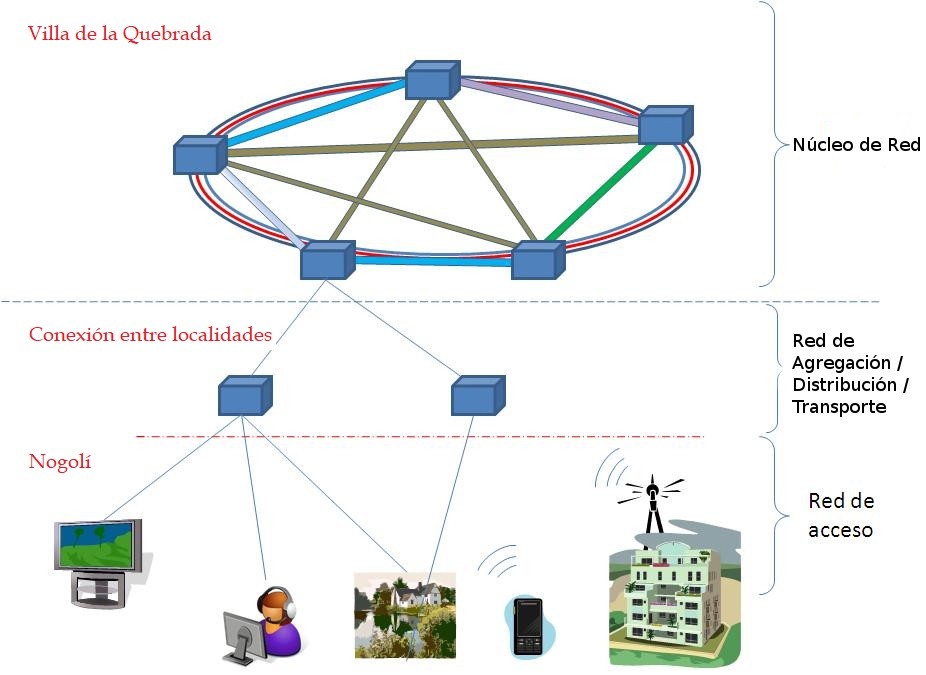
\includegraphics[width= 12 cm]{../figuras/red_transporte_1.jpg}
\caption{Jerarquía de redes. Redes de Acceso, Ing. Juan Vanerio - 2017}
\label{fig_jerarquia_redes}
\end{figure}

\section{Radio Enlace}

\subsection{Pre-ingeniería de Enlace}

Para la selección de los equipos a utilizar en el Radio enlace punto a punto, se realiza un análisis de pre-ingeniería que tiene en cuenta la normativa, frecuencia y potencia. En las siguientes secciones se tendrá en cuenta el ancho de banda, la tasa de datos necesario, como así también, el tipo de modulación.

En principio, se decide optar por dispositivos de radio enlace punto a punto con frecuencias de operación del orden de los 5.2 GHz a los 5.8 GHz ya que en línea recta desde Villa de la Quebrada a Nogolí hay una distancia de 12.05 km, y la empresa Ubiquiti ofrece un amplio rango de antenas con buenas características para el enlace deseado, pero las normativas en la República Argentina no permiten superar 1 dBm de potencia en el rango de frecuencia mencionado, por lo cual se descartaron dichos equipos.

Para elegir un equipo que este dentro de las normas de Argentina, se hace uso de la Disposición 734/2004 de la CNC (actual ENACOM: Ente Nacional de Comunicaciones), que fija los criterios para el mejor uso del espectro de frecuencias radioeléctricas atribuido al servicio fijo en bandas superiores a 1000 MHz (sistemas multicanales punto a punto), siendo las bandas incluidas en la frecuencia de 7 GHz las elegidas para que los equipos operen. Además, con ayuda de la Resolución 253 CS/2001 que regula las bandas y canalizaciones para los Sistemas Multicanales Digitales (MXD), se tuvo en consideración que los anchos de bandas permitidor por regulación son de 7 MHz, 14 MHz y 28 MHz. Estas bandas se tienen en cuenta al momento de obtener la sensibilidad del receptor en las hojas de datos, para los cálculos.


\subsection{Selección de equipos}

Se encontraron varios dispositivos en la frecuencia de operación elegida de diferentes marcas como por ejemplo: Sky Links, SAF, SIAE, aunque la gran parte fueron descartados por falta de información; por lo cual se selecciona el equipo Cambium, dado que la hoja de datos contiene toda la información necesaria para realizar los cálculos de enlace y así poder dimensionar la red.

Se debe remarcar, que el equipo seleccionado debe conseguir una tasa de datos de como mínimo 240 Mbps en hasta 28 MHz de ancho de banda, para respetar la normativa vigente mencionada en la sección anterior y cubrir la tasa de datos necesaria para brindar el servicio a la Localidad de Nogolí, la cual fue calculada hasta el año 2025, como se analizó en la Sección %\label(sec_analisis_dem_soc).

\textbf{Cambium 820C PTP}


\textbf{Ventajas:}

\begin{itemize}
\item No requiere de espacio en rack;
\item Difícil acceso a IDU o ODU (por posibles saqueos);
\item Permite montaje directo ODU-Antena (menor pérdida por alimentador de guías de ondas);
\item Flexibilidad para multiples configuraciones;
	\begin{itemize}
	\item MultiCore 2+0 Doble o simple Polarización de montaje directo, Fig.\ref{fig_cambium_1};
	
\begin{figure} [H]
\centering
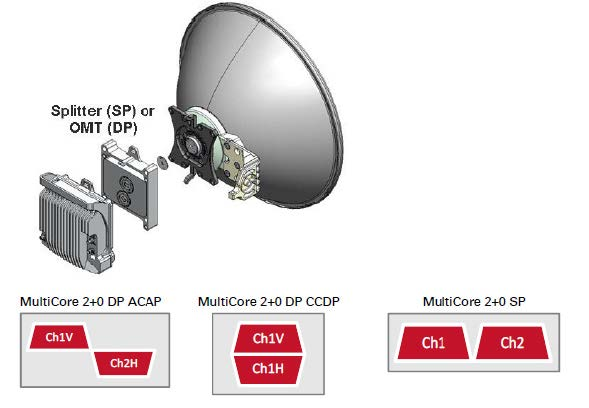
\includegraphics[width= 6cm]{../figuras/cambium_1.jpg}
\caption{Doble o simple polarización de montaje directo. Hoja de datos Cambium PTP 820C.}
\label{fig_cambium_1}
\end{figure}
	
	\item 2x MultiCore 2+0 Doble Polarización, Fig. \ref{fig_cambium_2};
\begin{figure} [H]
\centering
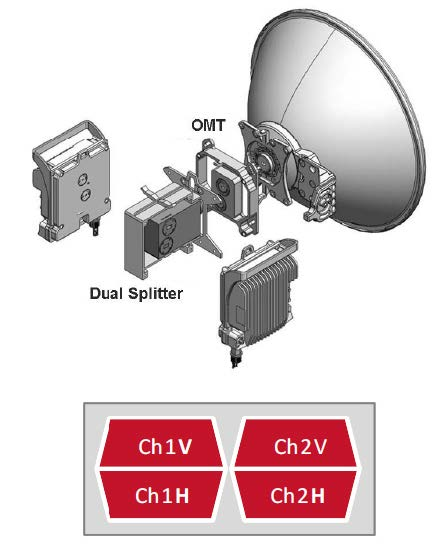
\includegraphics[width= 4cm]{../figuras/cambium_2.jpg}
\caption{Doble polarización. Hoja de datos Cambium PTP 820C.}
\label{fig_cambium_2}
\end{figure}	

	\item MultiCore 2+2 HDB Doble Polarización, Fig. \ref{fig_cambium_3}.
\begin{figure} [H]
\centering
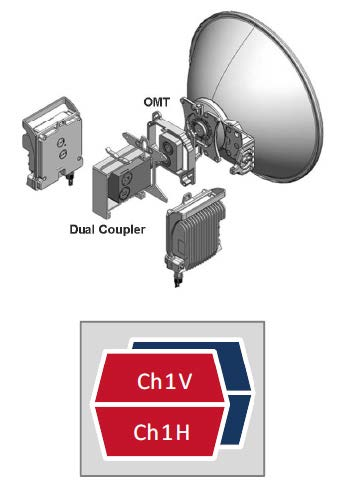
\includegraphics[width= 4cm]{../figuras/cambium_3.jpg}
\caption{HDB Doble polarización. Hoja de datos Cambium PTP 820C.}
\label{fig_cambium_3}
\end{figure}	

	\end{itemize}
\end{itemize}

\noindent\textbf{Desventajas:}
\begin{itemize}
\item Mantenimiento más complicado;
\item Personal con formación en altura para cualquier actuación;
\end{itemize}

A continuación, se presentan las características más importantes del dispositivo de radio enlace, además de la antena recomendada por el fabricante.

\medskip

\begin{table} [H]
\begin{center} 
\begin{tabular}{|c|c|c|c|}
\hline 
\multicolumn{4}{|c|}{\textbf{Parámetros Cambium 820C PTP (BW=28 MHz)}} \\ 
\hline 
\textbf{Modulación} & 2048 QAM & 1024 QAM (L FEC) & 1024 QAM (S FEC) \\ 

\hline 
\textbf{Potencia Tx} & 22 dBm & 24 dBm & 24 dBm \\
\hline
\textbf{Tasa de datos} & 241.31 Mbps & 224.96 Mbps & 211.89 Mbps \\
\hline
\textbf{Sensibilidad Rx} & -58 dBm & -61.5 dBm & -62.5 dBm \\
\hline
\textbf{Frecuencia de operación} & \multicolumn{3}{|c|}{\textbf{Rango Tx:} 7.105 - 7.164 GHz \textbf{Rango Rx:} 7.272 - 7.300 GHz} \\
\hline
\end{tabular} 
\label{tab_caracteristicas_cambium}
\caption{Características técnicas del equipos Cambium PTP 820C}
\end{center}
\end{table}

\medskip
\begin{table}[H]
\begin{center}
\begin{tabular}{|c|c|c|c|}
\hline
\multicolumn{4}{|c|}{\textbf{Parámetros Antenas Andrew}} \\
\hline
\textbf{Diámetro} & 0.6 metros & 1 metro & 1.2 metros \\
\hline
\textbf{Polarización} & Única & Única & Única \\
\hline
\textbf{Frecuencia de operación} & 7.1 - 8.5 GHz & \multicolumn{2}{|c|}{7.125 - 8.5 GHz} \\
\hline
\textbf{Ganancia} & 31.1 dBi & 35.3 dBi & 37.4 dBi \\
\hline
\textbf{Relación delante/atrás} & 57 dB & 61 dB & 63 dB \\
\hline
\textbf{Peso} & 21 kg & 46 kg & 74 kg \\
\hline
\end{tabular}
\label{tab_caracteristicas_antenas_andrews}
\caption{Características técnicas de las antenas Andrews}
\end{center}
\end{table}


\noindent\textbf{Pérdidas de dispositivos de conexión}

Para realizar los cálculos de enlace, se requiere conocer todas las perdidas que existen en el camino de la señal, una de estas pérdida se da en los dispositivos utilizados para interconectar el o los equipos utilizados. Para este equipo se requiere de un OMT (polarización vertical u horizontal), como puede verse en la Fig. \ref{fig_cambium_4} y un Splitter, vease Fig. \ref{fig_cambium_5}.

Según la hoja técnica del fabricante, las pérdidas son despreciables en estos dispositivos conectores para frecuencias del orden de los 6 GHz a los 8 GHz.



\begin{figure}[H]
\centering
\subfigure[OMT (pol V o H)]{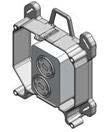
\includegraphics[width=4 cm]{../figuras/cambium_4.jpg}\label{fig_cambium_4}} 
\subfigure[Splitter]{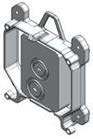
\includegraphics[width=3.5 cm]{../figuras/cambium_5.jpg}\label{fig_cambium_5}}
\caption{Dispositivos de conexión Cambium PTP 820C}
\end{figure}


\subsection{Análisis de enlace} 

En principio, se busca obtener el enlace de menor costo, es decir, un enlace punto a punto con un terminal en cada localidad sin necesidad de un repetidor, pero como puede verificar en el Anexo \ref{ane_calculo_red_trasporte}, debido a la imposibilidad del enlace mencionado se plantean otros dos enlaces con un repetidor entre localidad. 

El enlace seleccionado, se compone de un repetidor en la intersección de la ruta nacional RN146 y la ruta de acceso a Nogolí, en donde se tiene línea de vista y solo 5 km a Nogolí. Recordando, que uno de los radio enlaces se encuentra en Villa de la Quebrada y el otro en Nogolí.
La principal ventaja de colocar un repetidor cerca de una de las localidades, se basa en la necesidad de dar mantenimiento al equipo, tanto preventivo como correctivo, permitiendo tener una cuadrilla en Nogolí que se encargue del enlace que estaría a 5 km como así también dentro de la localidad.

Este enlace debe cumplir con la capacidad necesaria para el año 2025, que es de 222.9 Mbps para tener en cuenta el crecimiento de la población y del mercado ocupado.

Por lo mencionado anteriormente, se busca conseguir un enlace con una capacidad superior a 222.9 Mbps, como puede verse en la Tabla \ref{tab_caracteristicas_cambium}, el equipo permite obtener una capacidad de 225 Mbps con una modulación 1024 QAM, por lo cual en el programa "Radio Mobile " se utilizará la configuración para este tipo de modulación según los parámetros del dispositivo, que se encuentran en las Tablas \ref{tab_caracteristicas_cambium} y \ref{tab_caracteristicas_antenas_andrews}.


\subsubsection{Presupuesto de potencia}

Se prosigue a realizar el cálculo de las ganancias y pérdidas del sistema así como el presupuesto de potencia del enlace 1 (Villa de la Quebrada - Ruta 146; Ruta 146 - Nogolí).

Se utiliza la siguiente ecuación:

\begin{equation}\label{ec_presupuesto_potencia1}
G_{s}=P_{t} - C_{minima} \geq F_{m} + L_{p} + L_{f}+ L_{b} - A_{t} - A_{r}
\end{equation}

Donde:

\begin{itemize}
\item $G_{s}$: Ganancia del sistema (dB).
\item $P_{t}$: Potencia de salida del transmisor (dBm).
\item $C_{minima}$: Potencia mínima de entrada del receptor para un objetivo de calidad determinado (dBm).
\item $F_{m}$: Margen de desvanecimiento (dB).
\item $L_{p}$: Pérdida de la trayectoria de espacio libre entre antenas (dB).
\item $L_{f}$: Pértida del alimentador de guía de ondas (dB).
\item $L_{b}$: Pérdida total de acoplamiento o ramificación (dB).
\item $A_{t}$: Ganancia de antena transmisora (dBi).
\item $A_{r}$: Ganancia de antena receptora (dBi).
\end{itemize}

\noindent\textbf{Enlace: Villa de la Quebrada - Ruta 146/Acceso Nogolí}

En la hoja de especificaciones técnicas del equipo utilizado, Cambium PTP 820C, se indica que a una frecuencia de 7 GHz la potencia de salida del transmisor es de 24 dBm y que la sensibilidad de recepción para un ancho de banda de canal de 28 MHz es de -61.5 dBm, utilizando una modulación 1024 QAM.

La pérdida de trayectoria de espacio libre $L_{p}$ se define como:

\begin{equation}\label{Perdida_tratectoria}
L_{p}=(\frac{4 \pi f D }{c})^{2}
\end{equation}

Donde:

\begin{itemize}
\item $f$: Frecuencia de portada.
\item $c$: Velocidad de la Luz en el vacío.
\item $D$: Distancia entre antenas.
\end{itemize}

Si $f$ se expresa en GHz y $D$ en Km entonces $L_{p}$ resulta en dB como sigue:

\begin{equation}\label{perdida_trayectoria_db}
L_{p}[dB]=92.4 + 20 \log{f} + 20 \log{D}
\end{equation}

Por consiguiente, se obtiene

\begin{equation}\label{perdida_trayectoria_db_resultado}
L_{p} =92.4 + 20 \log{7.2} + 20 \log{13.5} = 132.15 [dB]
\end{equation}

En la hoja de especificaciones técnicas del equipo utilizado se indica que, a la frecuencia de 7 GHz las pérdidas por alimentador de guía de ondas ($L_{f}$) y la pérdida total de acoplamiento ($L_{b}$) son despreciables.

Se utilizan dos antenas VHLP3 de Andrew de 1 metro de diámetro con una ganancia de 35.3 dBi. Por lo tanto, $A_{t}=A_{r}= 35.3 dBi$.

El margen de desvanecimiento se define con la ecuación de confiabilidad de Barnett-Vignant, \ref{ec_Barnett}.

\begin{equation}\label{ec_Barnett}
F_{M}= 30 \log(D) + 10 log(ABf)- 10 \log(1-R) - 70 [dB]
\end{equation}

Donde:

\begin{itemize}
\item $D$: Distancia entre antenas [Km]: 13.5 Km.
\item $f$: Frecuencia central [GHz]: 7.2 GHz.
\item $R$: Confiabilidad expresada como decimal.
\item $A$: Factor de rugosidad: 1 textbf{(terreno normal)}.
\item $B$: Factor de corrección: 0.25 texbf{(Áreas normales tierra adentro)}.
\end{itemize}

Se define una confiabilidad del 99.9\% anual, lo que equivale a 8 hs y 45 min en el que el enlace puede estar fuera de servicio en un año.

El margen de desvanecimiento calculado es

\begin{equation}\label{Barnet_resultado}
F_{M}= 30 \log(13.5) + 10 log(6 * 1 *0.25*7.2)- 10 \log(1-0.999) - 70= 4.24 [dB]
\end{equation}

En Fig. \ref{fig_red_transporte_3}, se expone que el margen de desvanecimiento obtenido en el enlace es 22 dB, esto se debe en parte a que en la ecuación utilizada se tiene en cuenta un 60\% de la primer zona de Fresnel liberada, y en Radiomobile se ha liberado el 100\% de la primer zona. Esto indica que con la confiabilidad propuesta, se puede tener un margen de desvanecimiento de 4.24 dB y el enlace, teóricamente, se encontrará en funcionamiento el 99.9\% del año. Se considera como buena práctica utilizar un margen de desvanecimiento mayor a 20 dB.

Se prosigue a calcular la ganancia mínima del sistema

\begin{equation}
G_{s}=4.24 + 132.15 - 2 * 35.3 = 67.79 [dB]
\end{equation}

Por lo tanto, la diferencia entre la potencia de transmisor y la sensibilidad del receptor debe ser mayor o igual a 65.79 dB. En este caso se tiene que la ganancia del sistema es

\begin{equation}
G_{s_enlace}= 24 + 61.5 = 85.5 [dB]
\end{equation}

Se observa que la ganancia de sistema del enlace 1.a es superior a la calculada teóricamente, por consiguiente se considera que es un enlace robusto.

\medskip

\noindent\textbf{Enlace: Ruta 146/Acceso Nogolí - Nogolí}

En el presente enlace se utiliza la misma modulación y canalización que en el enlace Villa de la Quebrada – Ruta 146/Acceso Nogolí, por lo tanto

$P_{t}:24 dBm; C_{minima}=-61.5 dBm$

En Fig. \ref{fig_red_transporte_5} se expone que la distancia entre antenas es de 4.92 km (para realizar los cálculos se redondea a 5 km).

Se utilizan dos antenas VHLP3 de Andrew de 60 cm de diámetro con una ganancia de 31.1 dBi.

El margen de desvanecimiento es

\begin{equation}\label{Barnet_resultado_enlace1_b}
F_{M}= 30 \log(5) + 10 log(6 * 1 *0.25*7.2)- 10 \log(1-0.999) - 70= -8.6967 [dB]
\end{equation}

Se observa que el valor es negativo, este valor es causado por la confiabilidad elegida dado que depende en forma logarítmica de dicho valor.

Se calcula la pérdida de trayectoria de espacio 

\begin{equation}\label{perdida_trayectoria_db_resultado_1b}
L_{p} =92.4 + 20 \log{7.2} + 20 \log{5} = 123.52 [dB]
\end{equation}

Se prosigue a calcular la ganancia mínima del sistema

\begin{equation}
G_{s}=-8.7 + 123.52 - 2 * 31.1 = 52.62[dB]
\end{equation}

Por lo tanto, la diferencia entre la potencia de transmisor y la sensibilidad del receptor debe ser mayor o igual a 52.62 dB. En este caso se tiene que la ganancia del sistema es

\begin{equation}
G_{s_enlace}= 24 + 61.5 = 85.5 [dB]
\end{equation}

Se observa que la ganancia de sistema del enlace 1.b es muy superior a la calculada teóricamente, por consiguiente se considera que es un enlace robusto.

\subsubsection{Costo de enlace}
Para realizar la instalación del radio enlace antes planteado, se van a requerir de 3 torres, 2 de 6 metros y una de 14 metros para así poder respetar la altura de las antenas del Enlace 1. %El enlace se lleva a cabo utilizando un total de 4 antenas, 2 que se utilizan como terminales y 2 como repetidores.

Como puede verse en la Fig. \ref{fig_red_transporte_16}, los 4 equipos Cambium PTP 820C forman parte del enlace troncal teniendo un equipo en la Localidad de Villa de la Quebrada, donde se deberá alquilar/comprar un terreno para la colocación de la antena de 14 metros, lo mismo ocurre en el sector donde se encontrará el repetidor, como así también en la localidad de Nogolí.

\medskip
En principio, sólo se pensó en alquilar torres ya instaladas en ambas localidades pero esto depende completamente de la disposición del propietario en dar una pequeña porción de la torre para la instalación del equipo, corriendo el riesgo de que las alturas alquilados en las torres no sean los convenientes para el correcto funcionamiento del enlace; por esta razón y teniendo en cuenta que son torres de alturas relativamente bajas (costo reducido) se opta por realizar la compra de torres.


\begin{figure}
\centering
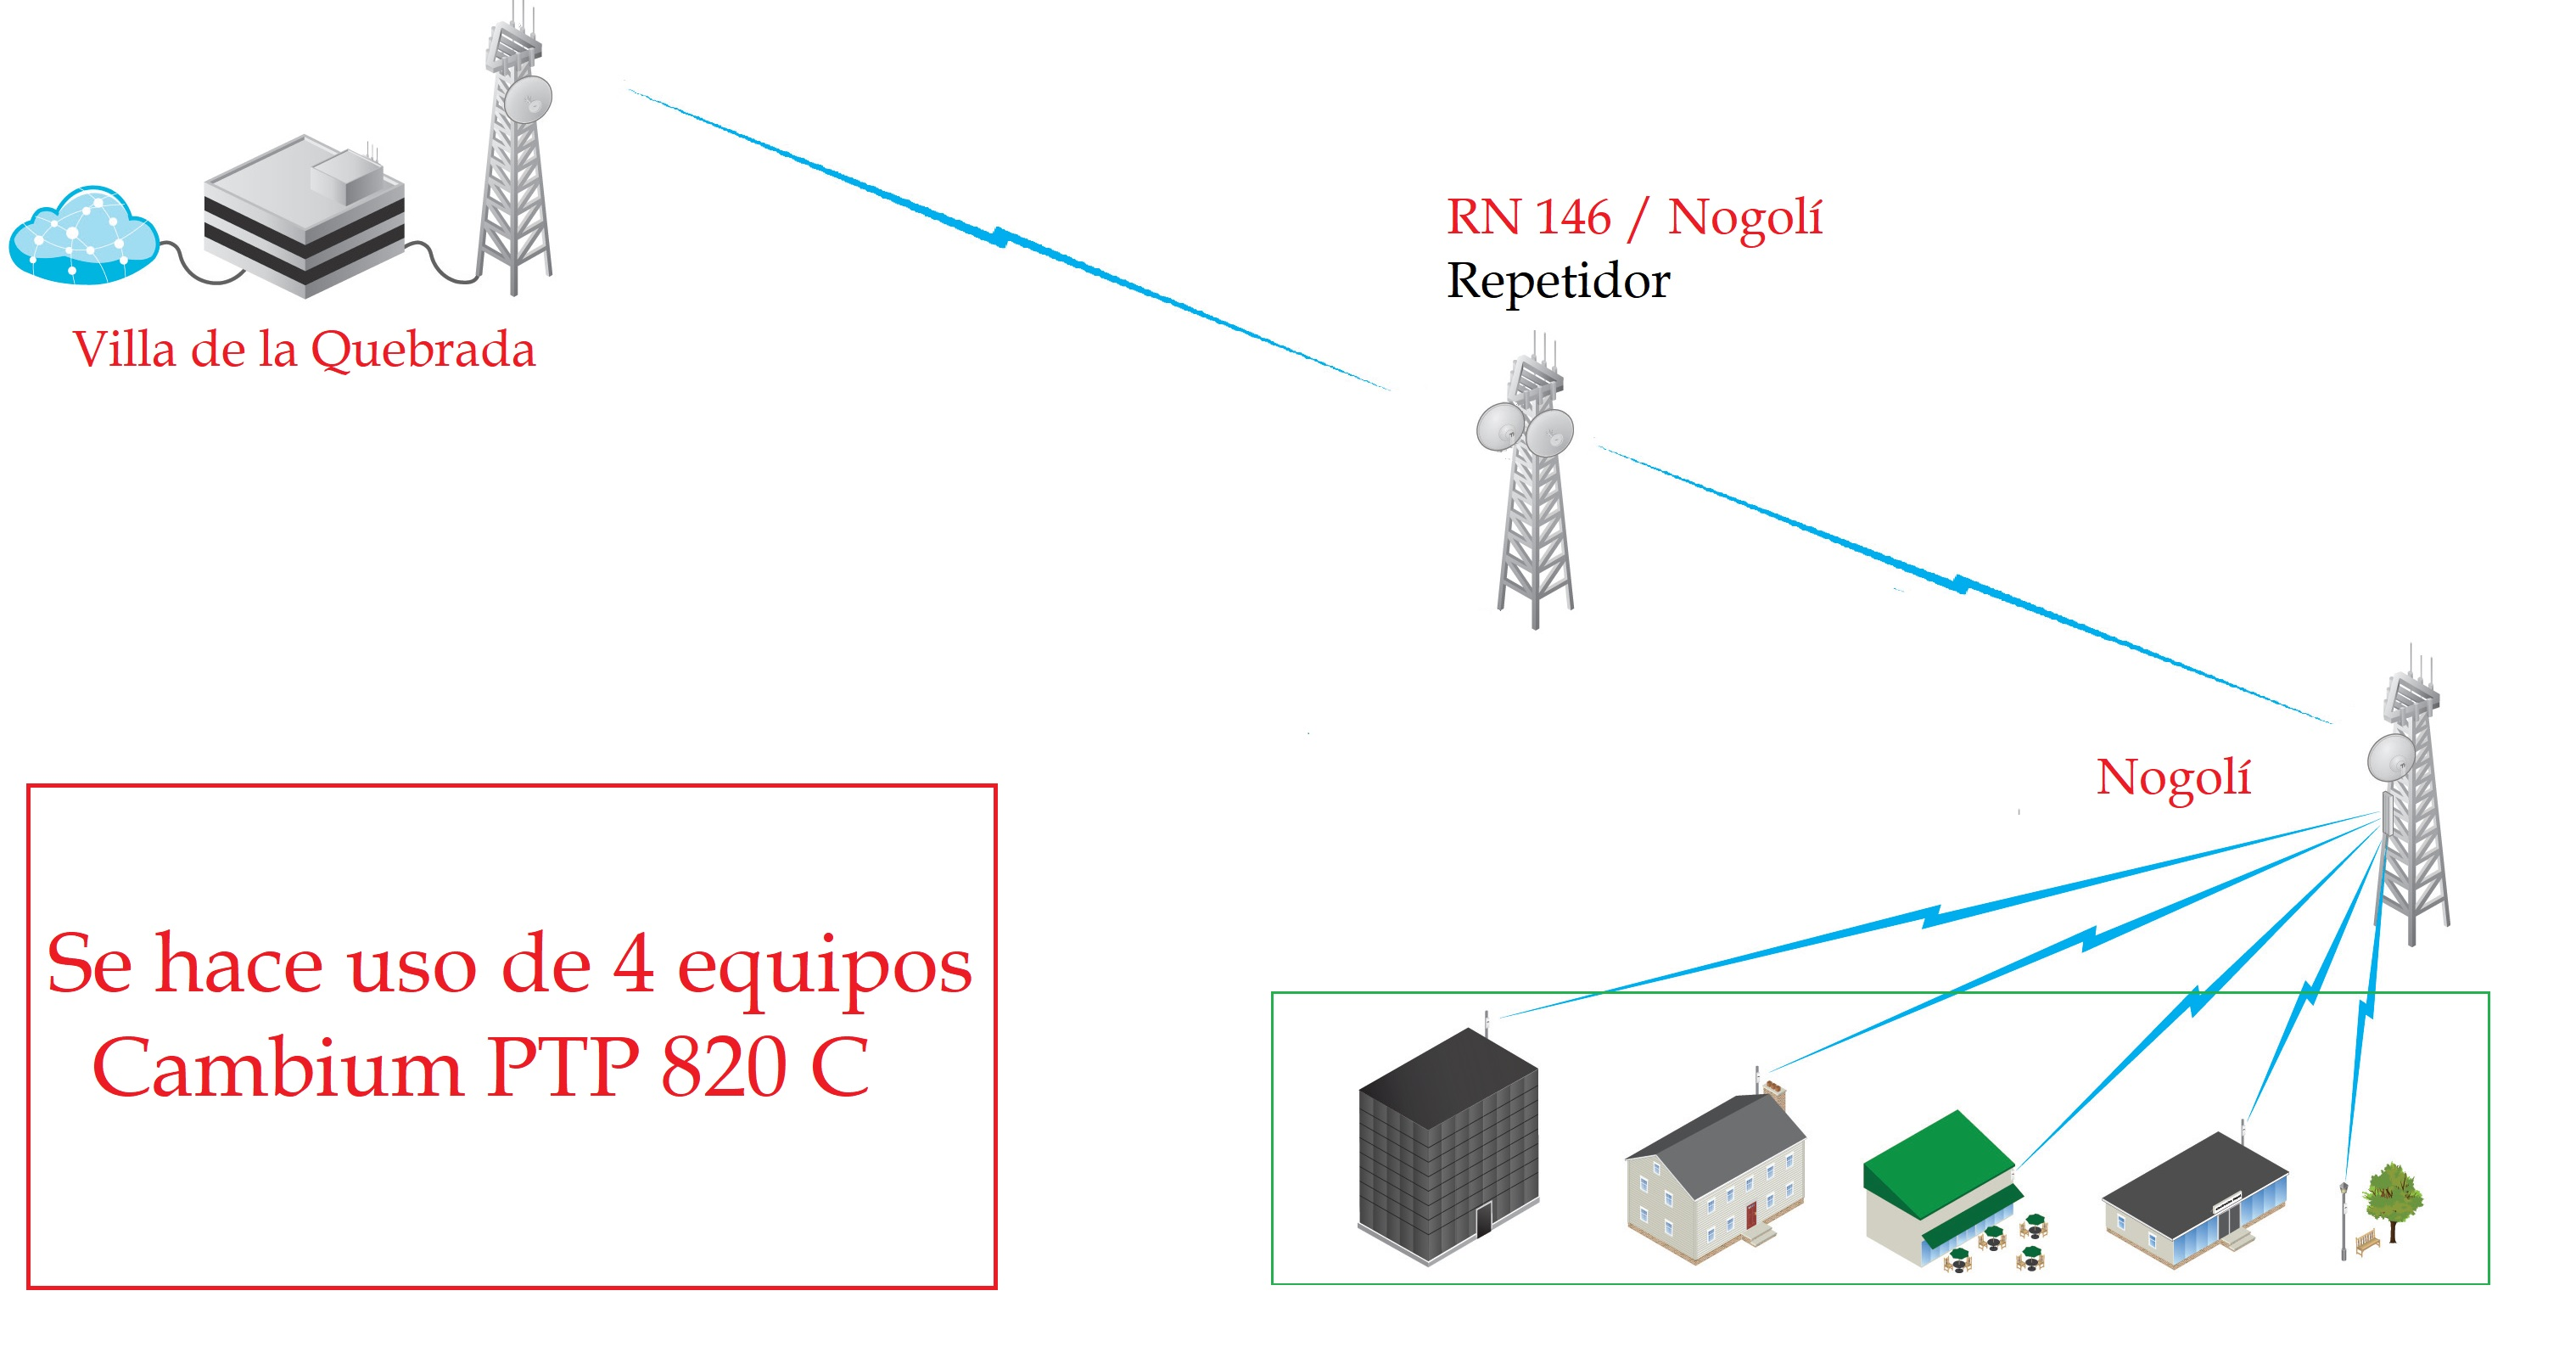
\includegraphics[width= 12 cm]{../figuras/red_transporte_16.jpg}
\caption{Configuración general del radio enlace 1.}
\label{fig_red_transporte_16}
\end{figure}

Teniendo en cuenta que el equipo de Cambium tiene un peso de 6.5 kg y la antena de Andrew de 1 metro un peso de 17 kg, se deben comprar 3 torres, dos de 6 metros y una de 15 metros, que soporten un peso de 25 kg a una altura de 5 metros y 12 metros, respectivamente. La empresa Torrenor S.A. de San Miguel, Buenos Aires, se encarga de dimensionar y presupuestar las 3 torres

La empresa Torrenor se encarga de dimensionar y presupuestar las 3 torres triangulares recomendando utilizar hierro redondo liso de 10 mm y zigzag de 8 mm, provistas con riendas de cable de acero de 3 mm y pintado reglamentario. 
En Fig. \ref{fig_red_transporte_17}, puede verse un trabajo de la empresa a modo de ilustrar las torres requeridas.

\begin{figure}
\centering
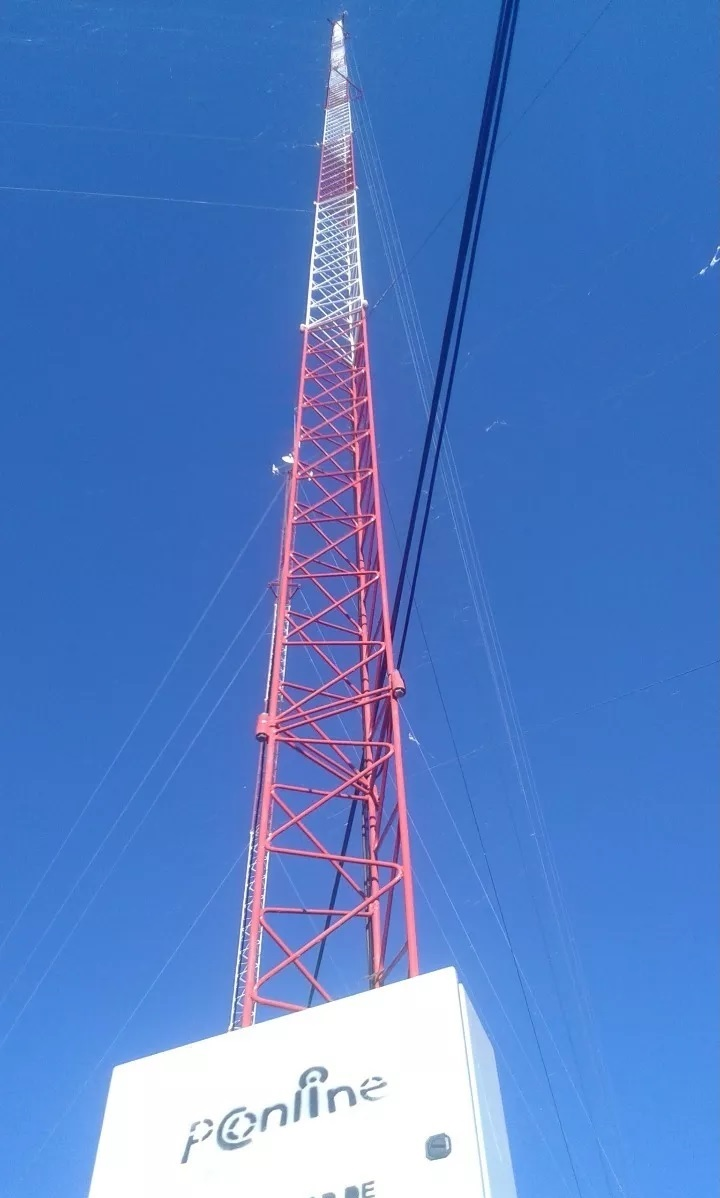
\includegraphics[width= 6 cm]{../figuras/red_transporte_17.jpg}
\caption{Torre fabricada por la empresa Torrenor.}
\label{fig_red_transporte_17}
\end{figure}


\begin{table} [H]
\begin{center}
\begin{tabular}{|c|c|c|c|c|}
\hline 
Producto & Cantidad & Precio & Total Parcial & Referencia \\ 
\hline 
Cambium PTP 820C & 4 & 5975 USD & 23900 USD & \ref{cost_radio_1}\\ 
\hline 
Andrew VHLP3-7W-2WH/A & 1 & 1315 USD & 1315 USD & \ref{cost_radio_2}\\ 
\hline 
Andrew VHLP2-7W-2WH/C & 3 & 550 USD & 1650 USD & \ref{cost_radio_2}\\ 
\hline 
Torre 6 metros & 2 & 160 USD & 320 USD & \ref{cost_radio_3}\\ 
\hline 
Torre 15 metros & 1 & 400 USD & 400 USD & \ref{cost_radio_3} \\ 
\hline 
\end{tabular} 
\end{center}
\caption{Costos de equipos de la Red de Transporte}
\label{tabla_precios_transp}
\end{table}


\subsubsection{Referencias de precios}
\begin{enumerate}
\item \label{cost_radio_1} 
\begin{verbatim} https://www.streakwave.com/itemdesc.asp?ic=C110082B029A \end{verbatim} 
\item \label{cost_radio_2}
\begin{verbatim} http://www.alldataresource.com/ \end{verbatim}
\item  \label{cost_radio_3}
 \begin{verbatim} https://articulo.mercadolibre.com.ar/MLA-605218700-torre-30-metros-torrenor-_JM \end{verbatim}

\end{enumerate}

\section{Fibra óptica}

Anteriormente, se realizó el diseño de la red troncal utilizando un radio enlace, en el cual se requiere de 4 antenas (al utilizar un repetidor). En este caso, para tener la posibilidad de comparar distintas tecnologías, se realiza el cálculo de un enlace troncal con fibra óptica.

Pero, ¿por qué fibra óptica?. El concepto de las comunicaciones por ondas luminosas ha sido conocido por muchos años.
Sin embargo, no fue hasta mediados de los años setenta que los estudios indicaron que era posible confinar un haz luminoso en una fibra transparente y flexible, y proveer así un medio óptico similar al de la señalización electrónica mediante alambres.
El problema técnico que había que resolver residía en las mismas fibras de vidrio portadoras: el vidrio ordinario tiene un haz luminoso de pocos metros, lo que dificultaba el proceso en la práctica, puesto que las señales deben ser transmitidas por muchos kilómetros.
Se desarrollaron entonces nuevos vidrios muy puros con transparencias mucho mayores, lo que fue un gran avance que le dio ímpetu a la industria la fibra óptica.
Por otro lado, como fuentes lumínicas se usaron láser o diodos emisores de luz, que debieron ser miniaturizados para ser componentes de los sistemas fibro-ópticos, lo que exigió una considerable labor de investigación y desarrollo. \footnote{Fuente: https://cie.gov.ar/web/images/Fibra-optica.pdf}

La gran ventaja de utilizar textbf(Fibra óptica), en vez de otro medio de trasmisión no solo tiene que ver con la gran tasa de datos que es posible obtener (1+ Gbps, en grandes distancias) sino también por su pequeño tamaño, peso y flexibilidad. Además, es inmune a ruidos e interferencias RF, la atenuación es reducida y controlable, la utilización puede ser independiente de la distancia. Se puede decir que la duración técnica es de aproximadamente 25 años, y por último, el costo es accesible y descendente en el tiempo. Una desventaja, la manipulación debe ser cuidadosa y por personal capacitado.

\subsection{Pre-Ingeniería de enlace}\label{subsec_pre_ing_enlace_fo_trans}

Siendo que se desea implementar un enlace troncal de distancia considerable (en comparación con las distancias que permiten las fibras multi-modo), se elige utilizar una fibra óptica de tipo mono-modo, ya que éstas permiten mayores distancias.

Los estándares analizados vigentes para fibras mono-modo, recomendados por la UIT-T, se exponen a continuación.

\begin{itemize}
\item \textbf{UIT-T G.652:} fibra monomodo estándar de dispersión no desplazada. Se optimizó inicialmente para su uso en la región de 1310 nm de longitud de onda, pero también puede ser utilizada en la región de 1550 nm. Es la fibra óptica más comercializada, su limitante es la dispersión cromática que afecta la región donde opera DWDM (3er ventana).

\item \textbf{UIT-T G.654:} está optimizada para operar en la región de 1500 nm a 1600 nm. Esta fibra presenta una baja pérdida y alta dispersión cromática en la banda de 1550 nm. Puede soportar mayores niveles de potencia y tiene un núcleo más grande. Se ha diseñado para enlaces submarinos de larga distancia.

\item \textbf{UIT-T G.655:} optimizada para operar en la banda de 1550 nm. Presenta poca dispersión cromática, minimizando los efectos no lineales que se ven en la multiplicación por división de longitud de onda densa (DWDM). Para el rango de 1530-1565 nm puede tener desde 1 hasta 10 ps/nm por kilómetro. Esto permite la operación de equipos sin necesidad de emplear dispositivos compensadores de dispersión, por lo que suelen emplearse en redes dorsales.

\item \textbf{UIT-T G.656:} fibra con dispersión no nula para el transporte óptico de banda ancha, optimizado para la operación en el rango de longitud de onda de 1460-1625 nm, manejando valores de dispersión cromática desde 1 hasta 14ps/nm por kilómetro, permitiendo utilizar CWDM y DWDM. Está diseñada para redes dorsales de alta capacidad.
\end{itemize}

Hay modelos que no pueden ser candidatos para el enlace que se plantea realizar, por ejemplo, el G.654 se ha diseñado para enlaces submarinos de larga distancia.

Se eligen las fibras bajo los estándares G.652 y G.655 ya que permiten la operación en 1310 nm siendo compatibles con el enlace que se desea realizar (12.5 km) y con los transceptores que se eligen en los puntos subyacentes. Además, G.652 es el estándar comercial más utilizado para la implementación de enlaces ópticos troncales.


Las fibras comerciales pre-seleccionadas son:
\begin{itemize}
\item Furukawa identificada como CFOA-SM-AS80-G-6
\item AFL identificada como Mini-Span 424 (ADSS)
\end{itemize}

Se decide analizar las fibras antes mencionadas, ya que los fabricantes han sido recomendados por profesionales con experiencia en este tipo de red. Así mismo las características determinantes en la selección de las mismas son:

\begin{itemize}
\item Cable de fibra óptica con recubrimiento en acrilato;
\item Fibra monomodo;
\item Auto soportado, con un vano máximo de 80 metros;
\item Cantidad de fibras ópticas: 6 fibras;
\item Según datasheet responde a los estándares G.652 y G.655.
\end{itemize}


\subsection{Elección de equipo}\label{subsec_eleccion_equipo_fibra}

Al utilizar fibra óptica mono-modo debido a la distancia entre transmisor y receptor, se hace uso de transceptores dotados de un diodo láser. El haz que emite un diodo láser es monocromático, direccional y coherente.

\begin{itemize}
\item \textbf{Monocromático:} de una sola longitud de onda. Mejor dicho, de un ancho espectral estrecho.
\item \textbf{Direccional:} patrón de radiación contenido en una región angular pequeña, haciendo que el acople con fibras mono-modo se realice de forma más fácil y eficiente.
\item \textbf{Coherente:} Todas las ondas individuales están en fase una con la otra en cada punto.
\end{itemize}

Según lo mencionado anteriormente, se elige el transceptor “Cisco glc-fe-100ex”, el cual presenta las siguientes características destacables:

\begin{itemize}
\item \textbf{Potencia Tx máx:} 0dBm
\item \textbf{Potencia Tx min: }-5 dBm
\item \textbf{Sensibilidad del receptor:} -34 dB
\item \textbf{Longitud de onda de operación:} 1310 nm
\item \textbf{Longitud de enlace máxima:} 40 km.
\item Interface con conector LC
\item Permite implementar SDH/SONET, Fast Ethernet, otros enlaces ópticos.
\end{itemize}

La elección del presente equipo se debe a la distancia de enlace que permite, la longitud de onda con la que opera y a la información que brinda el fabricante, ya que es muy importante tener acceso a las características del equipo para el diseño del enlace. Así mismo, se opta por utilizar un equipo de Cisco ya que ofrece un paquete de programas de simulación y supervisión determinante a la hora de su elección.

Se destaca que Cisco dispone de tranceptores con mayores tasa de datos que el seleccionado, pero así también con precios más elevados; siendo conveniente la elección de 3 tranceptores (sección \ref{subsec_presupuesto_potencia_fibra}) con menores tasas que cumple con las expectativas y proyecciones para el enlace troncal. 

\subsection{Análisis y elección de enlace}

Debido al tendido eléctrico de media tensión que se encuentra instalado en la autopista 25 de mayo, la cual une directamente Villa de la Quebrada con Nogolí, se plantea utilizar los postes para la implementación del tendido de fibra óptica, con cable óptico aéreo auto-soportado ya que permite un ahorro en la instalación del enlace teniendo en cuenta que la infraestructura ya se encuentra construido. En Fig. \ref{fig_red_transporte_14}, se expone una captura realiza con Google Earth de la zona de estudio. La distancia entre estos puntos es de 12.5 km.

\begin{figure} [H]
\centering
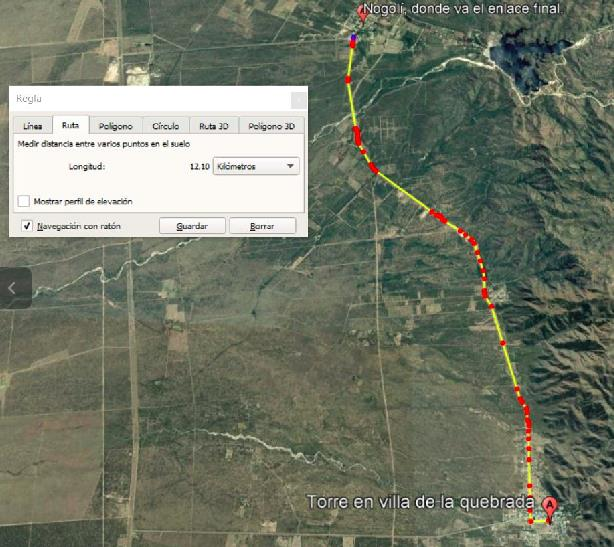
\includegraphics[width= 8 cm]{../figuras/red_transporte_14.jpg}
\caption{Vista satelital enlace fibra óptica}
\label{fig_red_transporte_14}
\end{figure}

La longitud total de la fibra, necesaria para el enlace, no solo está dada por la distancia medida anteriormente, sino que también debe tener en cuenta la ganancia de fibra, para futuros empalmes en el camino de la misma, y la curva que toma el cable entre los postes de amarre (catenaria). Según los documentos técnicos, la ganancia de fibra que se elige es del 15\% de la longitud máxima de la fibra, considerando la catenaria.

Para el cálculo de la catenaria, se parte de los siguientes datos:
• Fibra: Furukawa CFOA-SM-AS80-G-6:
	- Peso: 0.1 Kg/m,
	- Tensión máxima soportada: 2100 N, se toma 1800 N para no operar sobre el límite, dejando un margen de seguridad.
La distancia entre vanos, calculada usando la herramienta de medición de Google Earth, Fig. \ref{fig_red_transporte_15}, es de 65 metros.


\begin{figure} [H]
\centering
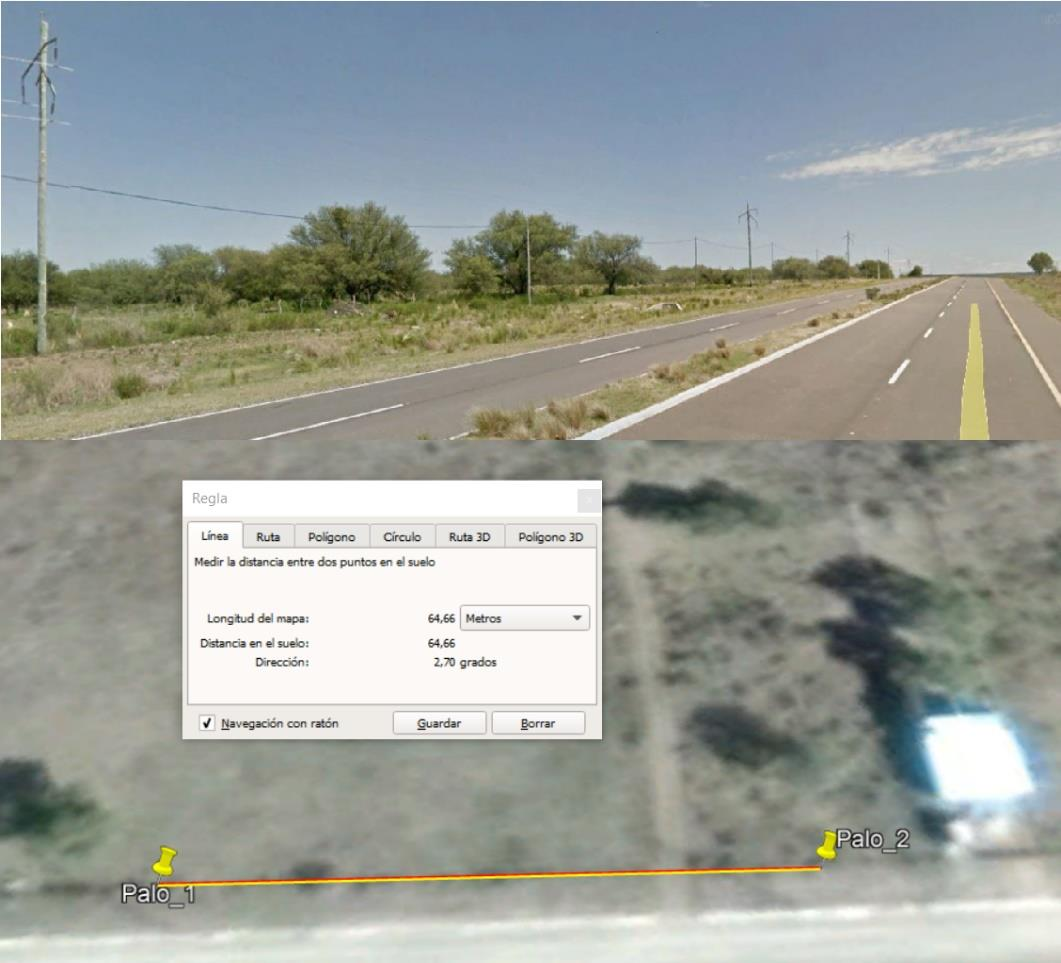
\includegraphics[width= 8 cm]{../figuras/red_transporte_15.jpg}
\caption{Distancia entre palos de media tensión. Usando Google Maps.}
\label{fig_red_transporte_15}
\end{figure}

Haciendo uso de una calculadora online de catenaria (Link Calculadora: https://www.easycalculation.com/es/analytical/cable-sag-error.php), y mediante los datos antes mencionados, se obtienen los siguientes resultados:

\begin{itemize}
\item Flechas (desde centro a curvatura máxima): 0.93 metros
\item Longitud de sección: 65.04 metros
\end{itemize}

Considerando la catenaria, la longitud entre vanos crece 0.04 metros por vano, este cambio debe ser trasladado a toda la instalación.

\begin{itemize}
\item Cantidad de vanos: $\frac{12500 m}{65 m} \cong 193 vanos$
\item Longitud del enlace: 193 vanos * 65.04 metros= 12553 metros
\end{itemize}

Por último, a la longitud del enlace debe agregarse la ganancia de fibra del 15 \%.
\begin{itemize}
\item Longitud total del enlace: 12553 m*1.15 =14436 m= 14.436 km.
\end{itemize}

\subsubsection{Presupuesto de potencia} \label{subsec_presupuesto_potencia_fibra}

El cálculo de enlace, o presupuesto de potencia, se define en la siguiente desigualdad, la cual se debe cumplir para que el enlace cumpla los requisitos mínimos que se han definido.

\begin{equation} \label{ec_presupuesto_potencia_fibra}
P_{th}+P_{ISI} \leq W - (N_{1}*A_{c}) - (N_{2}*L*A_{e}) - (A_{fo}*L) - (M_{c}*A_{e}*L) - M_{e}
\end{equation}

En la siguiente tabla, se expone el significado de los parámetros utilizados (ver Tabla \ref{tab_presuesto_potencia}.

\begin{table}
\centering
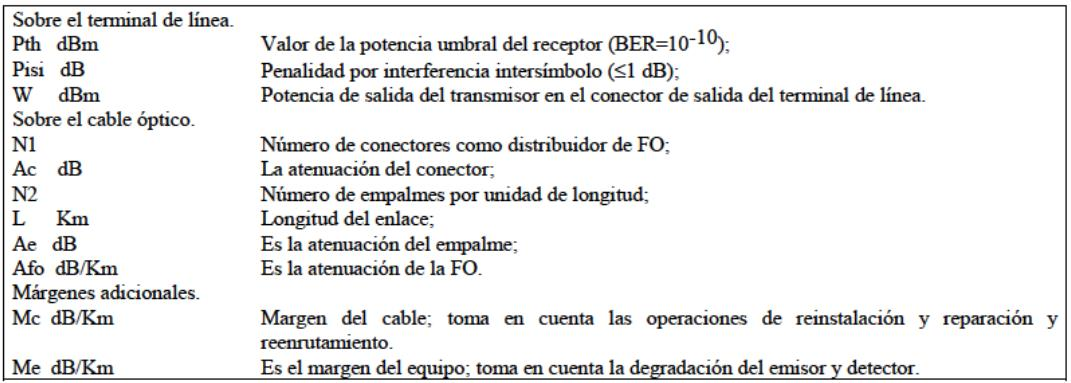
\includegraphics[width= 8 cm]{../figuras/table_fibra.jpg}
\caption{Vista satelital enlace fibra óptica}
\label{tab_presuesto_potencia}
\end{table}

\textbf{Sobre el terminal de línea:}

La sensibilidad del receptor del transceptor Cisco glc-fe-100ex es de -34dBm y la potencia de transmisión es de 0dBm.

Sobre el cable óptico:

Se utilizan conectores LC, cuya atenuación ($A_{c}$) es de 0.1 dB. En el mercado se encuentran disponibles rollos de fibra de 4km, por lo tanto el número de empalmes por unidad de longitud ($N_{2}$) es de 0.25. La fibra óptica G.652 presenta una atenuación de 0.4 dB/km (valor que puede variar en la instalación de la fibra, pero se encuentra en el orden estimado) y la fibra G.655 presenta una atenuación de 0.38 dB/km.

Cabe destacar que se realizan los cálculos para la ventana de 1310 nm (longitud de onda de operación del transceptor).

Se prosigue a realizar el cálculo para la primera fibra (G.652).

\begin{itemize}
\item $P_{th}$=-34 dBm
\item $P_{ISI} \leq 1$ (\textit{despreciable})
\item $E=-5 dBm$ (Potencia de transmisión mínima, peor de los casos)
\item $N_{1}$= 2
\item $A_{C}$=0.1 dN(Conector LC)
\item $N_{2}=0.25$ (tramos de 4 km)
\item $A_{e}=0.1 dB$ (máximo valor tolerado)
\item $L$= 14.436 km
\item $A_{fo}$=0.4 dB/km
\item $M_{c}$=0.01 dB/km
\item $M_{e}$=9 dB
\end{itemize}

\begin{center}

\noindent$-34 \leq -5-(2*0.1)-(0.25*14.436*0.1)-(0.4*14.436)-(0.01*0.1*14.436)-9=$
\noindent $-20.36 - 34 \leq -20.36$
\end{center}

\medskip

Se observa que se cumple la desigualdad obteniendo un margen de 13.65 dB, por lo tanto, el enlace satisface ampliamente las condiciones requeridas.

Se prosigue a realizar el cálculo para la segunda fibra (G.655), en la cual varía su atenuación por kilómetro

\medskip

\noindent $(0.38 dB/km) -34 \leq 0-(2*0.1)-(0.25*14.436*0.1)-(0.38*14.436)-(0.01*0.1*14.436)-9=$

\noindent\begin{center}
$=-15.06-34 \leq -15.06$
\end{center}

Se cumple la desigualdad obteniendo un margen de 18.94 dB.

Se observa que ambas fibras satisfacen la ecuación de enlace ampliamente. Sin embargo, se elige la fibra G.652 ya que se encuentra optimizada para la operación en 1310 nm, que es la longitud de onda de operación del equipo elegido. A su vez, la G.655 se encuentra optimizada para la operación con DWDM para enlaces de larga distancia (mayores a 80 km), por este motivo no se justifica su utilización para el enlace propuesto.

El fabricante del transceptor asegura una tasa máxima de 155 Mbps con un enlace de 40 km. Teniendo en cuenta que la distancia requerida representa el 35\% de la máxima estipulada por el fabricante, que la tasa utilizada es de 100 Mbps con fibra de 6 hilos (3 transceptores para superar la tasa máxima calculada en los análisis previos, aproximadamente 250 Mbps) y que la dispersión cromática es despreciable a distancias bajas, se puede asegurar que la tasa de transmisión será la estimada de 300 Mbps.

Teniendo en cuenta los resultados en el cálculo de enlace, no sería necesario la utilización de un repetidor o amplificador ya que en la ecuación de enlace se observa que el margen es elevado, por lo que la señal llegaría al receptor con una potencia mucho mayor que la mínima (impuesta por la sensibilidad del mismo).

En conclusión, se realiza un enlace de 14.436 km entre Villa de la Quebrada y Nogolí, mediante fibra óptica mono-modo fabricada bajo el estándar ITU-T G.652.

\subsubsection{Costo de enlace}
Para presupuestar el enlace, se buscaron los precios de ambas fibras seleccionadas en la Sección \ref{subsec_pre_ing_enlace_fo_trans}. Luego de varios intentos sin éxito para obtener el valor de la FO de Furukawa, se optó por elegir directamente la ofrecida por la empresa AFL con las mismas características.

Antes de mencionar los aspectos importantes presupuestados para el montaje de la FO auto-soportada, es necesario destacar que los transceptores de marca Cisco que se utilizan para iluminar la fibra son módulos SFP (Small Form-factor Pluggable), los cuales deben ser utilizados con equipos que soporten esta tecnología. Se selecciona el Switch Catalyst WS-C6504-E (Fig. \ref{fig_Catalyst_6500}), el cual cuenta con slots para la conexión de 4 módulos SPF, dejando un slot liberado como alternativa de conexión para el ISP de la empresa o para permitir ampliar la red troncal en un futuro.

\begin{figure}
\centering
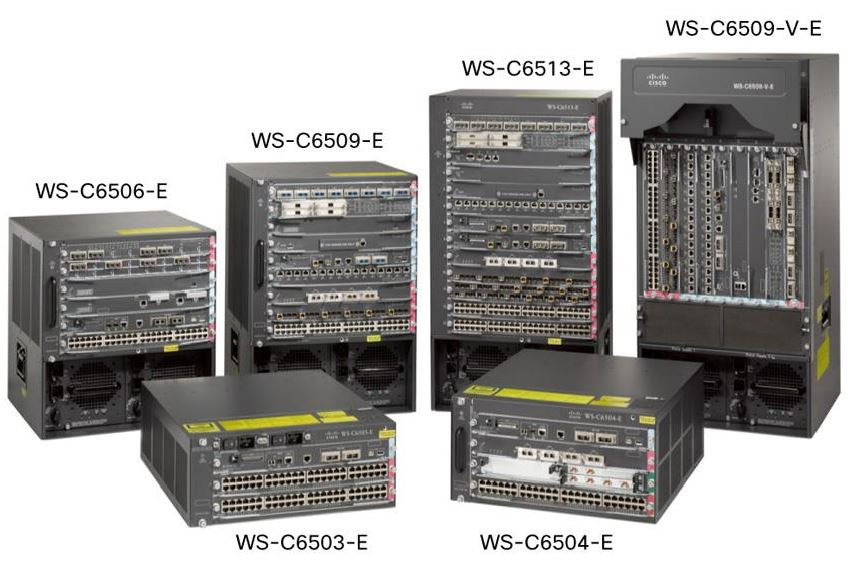
\includegraphics[width= 8 cm]{../figuras/Catalyst_6500.jpg}
\caption{Cisco Catalyst 6500-E Series Chassis. Fuente: Hoja de datos Catalyst 6500 E, Cisco.}
\label{fig_Catalyst_6500}
\end{figure}

Para la instalación de la FO en los palos de media tensión, desde la localidad de Villa de la Quebrada a Nogolí, se calculan 4 empalmes ya que se tiene una distancia entre localidades de aproximadamente 15 km, y la bobina de FO contiene 4 km. Para dichos empalmes, se requiere de 4 cajas de empalmes con soporte aéreo, ver Fig. \ref{fig_caja_empal_trans}. Cada dos vanos,es decir, unos 160 metros se colocan unidades de almacenamiento de fibra, ver Fig. \ref{fig_un_almace_trans}; permitiendo tener un margen por posibles averías del medio de transmisión.

\begin{figure}[H]
\centering
\subfigure[Caja de empalme con soporte aereo]{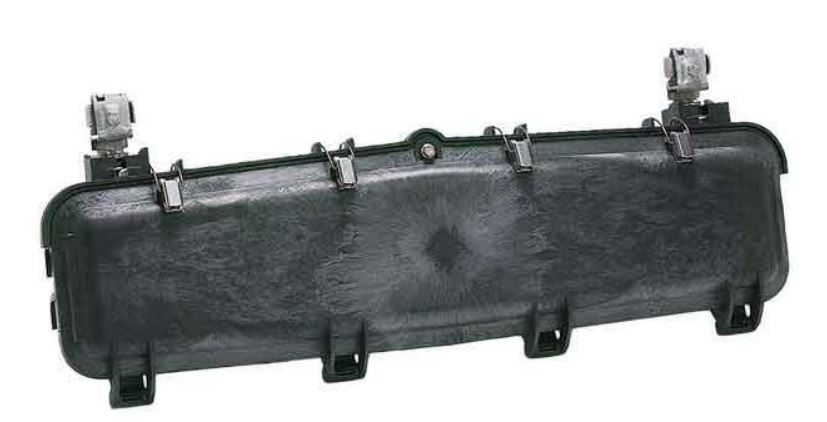
\includegraphics[width=4 cm]{../figuras/caja_empalme_FO_transporte.jpg}\label{fig_caja_empal_trans}} \thinspace
\subfigure[Unidad de almacenamiento de FO]{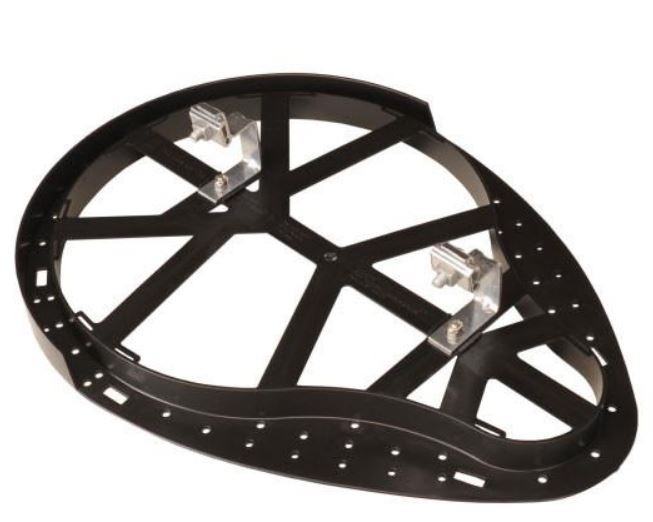
\includegraphics[width=3.5 cm]{../figuras/unidad_almacenamiento_FO.jpg}\label{fig_un_almace_trans}}
\caption{Accesorios de instalación}
\end{figure}

\begin{table}[H]
\centering
\begin{tabular}{|p{6cm} |>{\centering\arraybackslash}p{1.8 cm} |>{\centering\arraybackslash}p{2.5cm}| >{\centering\arraybackslash} p{2.5cm}| >{\centering\arraybackslash}p{2.5cm}|}
\hline 
\textbf{Producto} & \textbf{Cantidad} & \textbf{Precio} & \textbf{Total Parcial} &\textbf{ Referencias} \\ 
\hline 
FO AFL Mini-Span ADSS 424 & 15000 & 2.65 USD/m & 39750 USD & \ref{cost_FO_trans} \\ 
\hline 
Cisco Transceiver 100-BASE-EX & 6 & 15 USD & 90 USD & \ref{cost_transceiver_trans} \\ 
\hline 
Cisco Catalyst C-6504E & 2 & 2246 USD & 4492 USD & \ref{cost_switch_trans} \\ 
\hline 
LG 500 Aerial Compact Splice Closure & 4 & 175 USD & 700 USD & \ref{cost_caja_empalme_trans} \\ 
\hline 
Multilink Broadband 16" Plastic Sno-Shoe
 With Mounting Bracket And Hardware & 100 & 67 USD & 6700 USD & \ref{cost_un_almac_trans} \\ 
\hline 
Conector AFL LC (paquete de 6 unidades) & 2 & 172 USD & 344 USD & \ref{cost_conector_LC_trans} \\ 
\hline 
\end{tabular} 

\end{table}

\subsubsection{Referencias de precios}

\begin{enumerate}[{[1]}]
\item \label{cost_FO_trans} 
\begin{verbatim} https://www.fiberoptics4sale.com/collections/category_bulk-fiber-
cables/products/ae-00696c520-aa4 \end{verbatim} 
\item \label{cost_transceiver_trans}
\begin{verbatim} https://www.fiber-mart.com/100155mbps-100baseex-sfp-1310nm-40km-
transceiver-p-403.html \end{verbatim}
\item  \label{cost_switch_trans}
\begin{verbatim} https://www.ebay.com/p/Cisco-Catalyst-C6504-E-switch/74074274 \end{verbatim}
 \item  \label{cost_caja_empalme_trans}
\begin{verbatim} https://www.fiberoptics4sale.com/collections/subcategory_osp-fiber-
closures/products/fc000026 \end{verbatim}
\item  \label{cost_un_almac_trans}
 \begin{verbatim} https://www.fiberoptics4sale.com/collections/subcategory_fiber-slack-
storage/products/2116-ssptb \end{verbatim}
  
\item  \label{cost_conector_LC_trans}
 \begin{verbatim} https://www.fiberoptics4sale.com/collections/subcategory_fiber-optic-
 connectors/products/cs008237 \end{verbatim}

\end{enumerate}

\chapter{Red de Acceso}\label{cap_red_acceso}

Red de acceso hace mención a aquella parte de la red de comunicaciones que conecta a los usuarios finales con algún proveedor de servicios. En la actualidad es posible su implementación haciendo uso de diferentes tecnologías. En la presente sección, se plantea el estudio de pre-ingeniería, diseño y análisis de factibilidad tanto económica como técnica de dos tipos de red de acceso muy utilizadas; radio enlace y fibra óptica. Al final de la sección, con base en la información expuesta, se concluye la elección de la tecnología a utilizar.

 \medskip

Dado que se pretende brindar servicio de VoIP, HDTV y/o SDTV e Internet en dos paquetes, uno premium y uno estándar, se utiliza el servicio premium como base para el dimensionamiento de la red, ya que de esta forma se contempla un futuro crecimiento del mercado.

\medskip

\section{Radio enlace}\label{sec_radio_enlace_acc}

\medskip

Se comienza el análisis del radio-enlace realizando un estudio de pre-ingeniería enfocado a la disponibilidad de infraestructura para su implementación. Se analiza la distribución de viviendas en la zona, tendidos eléctricos y posibles ubicaciones de las antenas junto con las estaciones PtMP (Punto a Multipunto), así como la viabilidad de los enlaces mediante simulación.

\medskip

\subsection{Pre-Ingeniería de enlace}\label{subsec_acceso_pre_ing_enlace}

\medskip

Se recuerda al lector las características del servicio Premium, junto con las consideraciones realizadas.

\medskip

\begin{itemize}
\item 1 linea de telefonía IP (30 Kbps)
\item 1.5 televisores por hogar, con canal HD (6 Mbps por canal)
\item Conexión a internet (6 Mbps)
\end{itemize}

\medskip

La tasa requerida por vivienda será:

\medskip

\begin{equation}\label{ec_capacidad_premium}
Capacidad = [ 6 + 1.5 * 6 + 0.03] Mbps = 15.03 Mbps \approx 15 Mbps
\end{equation}

\medskip

Haciendo uso de la herramienta Google Maps se analiza la distribución de viviendas, dato que infiere directamente en la capacidad requerida por la red y en la cantidad de Access Points (Aps) a instalar.

\medskip

En Fig. \ref{Fig_Division_zonas_Nogoli} se expone una división por zonas, donde se indica la cantidad aproximada de viviendas y su distribución.

\medskip

\begin{figure} [H]
\centering
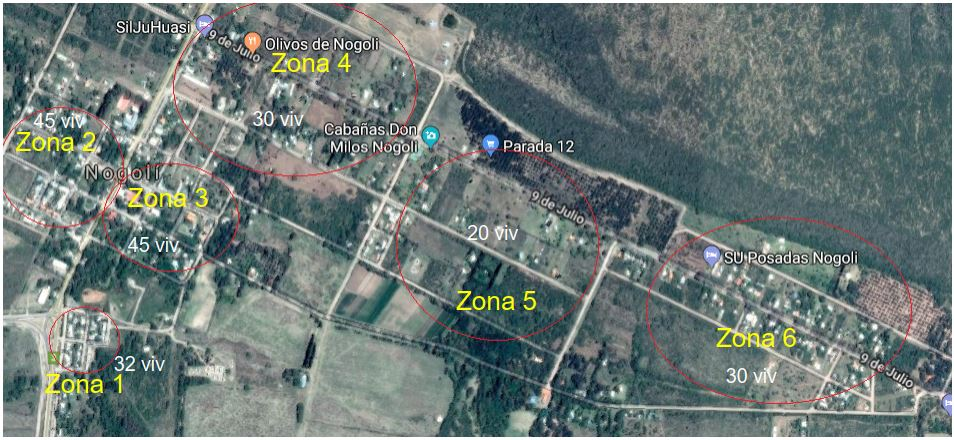
\includegraphics[width= 17cm]{../figuras/Div_por_zonas_Nogoli.JPG}
\caption{División por zonas de la localidad Nogolí. Google. (s.f.). [Mapa de Nogolí, San Luis - Argentina en Google maps]. Recuperado el 20 de Septiembre, 2018, de: https://www.google.com.ar/maps/@-32.9179974,-66.3166214,1492m/data=!3m1!1e3}
\label{Fig_Division_zonas_Nogoli}
\end{figure}

\medskip 

En sección \ref{cap_demografico} se ha estimado un total de 113 usuarios y utilizando un factor de re-uso de 1:4 (es conveniente ser conservador ya que no se conoce con exactitud la
concentración de usuarios por AP) se obtiene 29 usuarios. Esto indica que
se dimensiona la red para el caso en que el 25\% de los usuarios consuman el
máximo de su capacidad (15 Mbps) en simultáneo.

\medskip

En las siguientes subsecciones se utilizarán los datos aquí expuestos.

\medskip

\subsection{Pre-selección de equipos}\label{subsec_acceso_pre_selec_equipos}

Para el diseño de una red de acceso utilizando radio enlace se requiere de sistemas inalámbricos punto a multipunto y de equipos en los hogares para establecer la conexión. 
Se propone la operación en la banda no licenciada de 2.4 GHz ya que a esta frecuencia se logran mayores distancias en comparación con la banda de 5 GHz, a costa de una menor tasa de datos.

\medskip

Se elige la estación base punto a multipunto \textbf{Rocket M2 Titanium} de la empresa Ubiquiti Networks, Inc. En Anexo \ref{ane_comp_equipos_Radio_red_acceso} se expone una comparación entre las características de los equipos analizados y la justificación de la elección.
\medskip 

En Fig. \ref{Fig_Rocket_M2_T} se expone una ilustración de la estación base Rocket M2 Titanium.

\medskip

\begin{figure} [H]
\centering
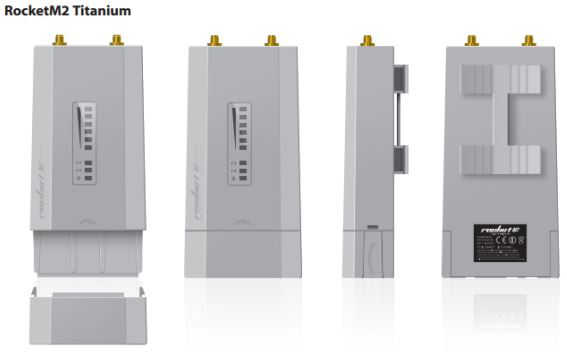
\includegraphics[width= 15cm]{../figuras/Rocket_M2_Titanium.JPG}

\caption{Base Station Rocket M2 Titanium. Hoja de datos Rocket M2 Titanium, Ubiquiti Networks, Inc. }
\label{Fig_Rocket_M2_T}
\end{figure}


\medskip

Se plantea el uso de una antena omnidireccional AMO-2G13, recomendada por Ubiquiti Networks Inc. la cual opera en el rango de 2.35 GHz – 2.55 GHz compatible con 2x2 MIMO y con airMAX, con polarización dual lineal y 13 dBi de ganancia. En Fig. \ref{Fig_patron_rad_antena} se expone el patrón de radiación de la antena. \medskip

\begin{figure} [H]
\centering
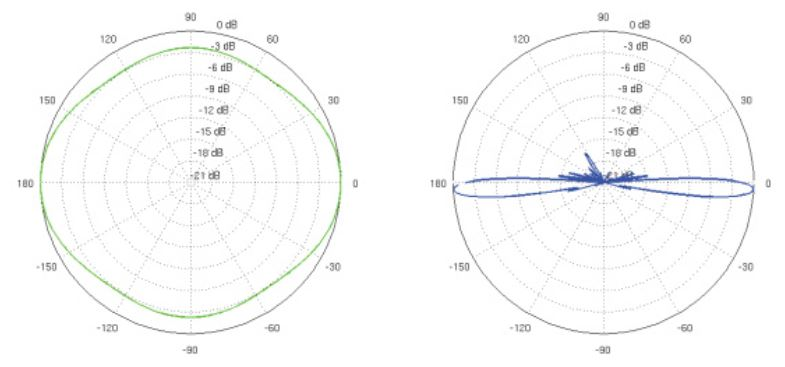
\includegraphics[width= 010 cm]{../figuras/patron_radiacion_amo_2g13.JPG}

\caption{Patrón de radiación vertical (izquierda) y horizontal (derecha). Hoja de datos AMO 2G13.}
\label{Fig_patron_rad_antena}
\end{figure}

Para establecer comunicación entre el usuario y el AP se utiliza una NanoStation Loco M2 (Fig. \ref{Fig_NSLocoM2}) fabricada por Ubiquiti Networks Inc., la cual opera en la banda de 2.4 GHz haciendo uso del protocolo Airmax (TDMA) y MIMO. Presenta 17 dBm de potencia de transmisión a una modulación Airmax MCS15 y -75 dBm de sensibilidad a la misma modulación, con una antena integrada de 8.5 dBi. Se plantea utilizar el presente equipo ya que al ser del mismo fabricante que la estación base, facilita la gestión de compra así como la compatibilidad permitiendo el uso del mismo software de supervisión.

\medskip

\begin{figure} [H]
\centering
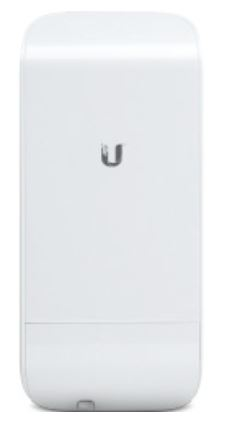
\includegraphics[height= 5cm]{../figuras/NanoStationLocoM2.JPG}
\caption{Nano Station Loco M2. Hoja de datos de NSLocoM2, Ubiquiti Networks Inc..}
\label{Fig_NSLocoM2}
\end{figure}

\medskip

\subsection{Análisis de enlace}\label{sub_analisis_enlace_acc}

Una vez definidos los equipos a utilizar, se prosigue a calcular la cantidad de APs (Base Station Rocket M2 Titanium) necesarios. Dado que la tasa de datos máxima del AP es 300 Mbps, se prosigue a calcular a cuantos usuarios con consumo de 15 Mbps puede brindar servicio el AP.

\begin{equation}\label{ec_CantUsuariosAP}
CantUsuarios = \frac{300}{15} = 20 
\end{equation}

Por lo tanto, con 2 AP se cubre el total de usuarios (recordar que se tienen 29 usuarios). Dicho análisis se realiza desde el punto de vista de la capacidad. 

\medskip

Es necesario tener en cuenta también la cobertura y la densidad de población en la localidad de estudio, ya que puede darse una congestión en un AP debido a una mala ubicación (ver Fig. \ref{Fig_Division_zonas_Nogoli}). Incluso, posiblemente se deba colocar más de dos APs. 

\medskip 
Se han realizado simulaciones para estimar la viabilidad de los enlaces, con enfoque en las características de los equipos (Potencias y sensibilidades), altura de instalación de antenas e interferencias; utilizando las herramientas WallMan y ProMan del software WinProp, dedicado a la simulación de propagación de ondas electromagnéticas en distintos entornos. En Anexo \ref{ane_simulacion_Radio_red_acceso} se exponen los resultados de la simulación. 

\medskip


Con base en los análisis realizados, se concluye la viabilidad técnica de la red de acceso implementada con la estación base \textbf{Rocket M2 Titanium} con antena omnidireccional \textbf{AMO-2G13} y \textbf{NanoStations Loco M2}. \medskip

Por último, se propone utilizar fibra óptica mono-modo para la conexión entre los APs y la red troncal. Con base en recomendaciones del fabricante de Fibra óptica Furukawa, en el documento \emph{Cables ópticos para proyectos FTTx}\footnote{Furukawa $(http://www.tecnoredsa.com.ar/productos/18ec73_cables.pdf)$ 5/10/2018}, se llega a la conclusión que el mejor tipo de fibra para la red de distribución es la que se encuentra bajo la norma ITU-T G.652. \medskip

Se opta por utilizar una topología tipo árbol con un nivel de splitter (1:8) y con fibra mono-modo Mini-Span ADSS 424 de AFL, permitiendo así la comunicación entre el equipo PtP de la red troncal y los 5 APs.

\medskip

En Fig. \ref{fig_redDistribucion_acceso} se expone una ilustración del tendido de fibra antes mencionado.

\medskip

\begin{figure} [H]
\centering
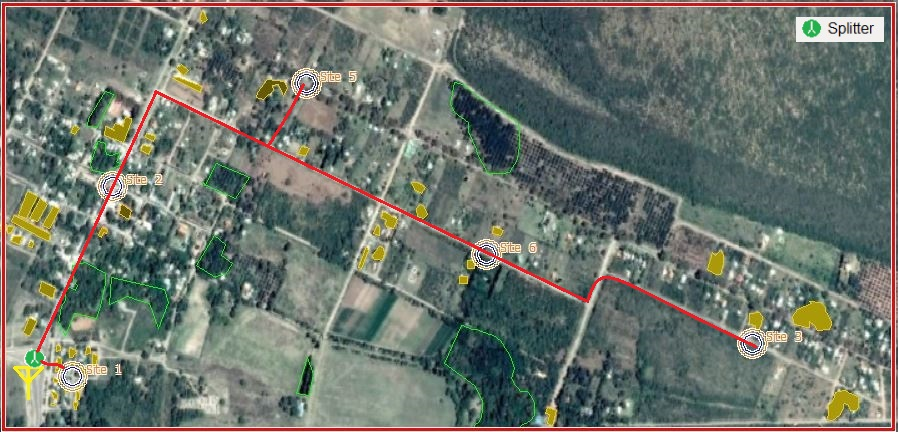
\includegraphics[width= 15cm]{../figuras/tendido_fibra_distribucion.JPG}

\caption{Red de distribución con fibra óptica.}
\label{fig_redDistribucion_acceso}
\end{figure}

\medskip

Se destacan las distancias entre los APs y la antena, dato que se utilizará en la siguiente subsección.

\medskip

\begin{itemize}

\item AP zona 1: 50 m
\item AP zona 2 y 3: 500 m
\item AP zona 4: 1250 m
\item AP zona 5: 1700 m
\item AP zona 6: 2500 m

\end{itemize}


\subsection{Costos de enlace}

Para la implementación de la red de acceso se requiere de 5 APs Rocket M2 Titanium con sus respectivas antenas AMO-2G13, 6.2 km de fibra óptica mono-modo Mini-Span ADSS 424 de AFL\footnote{Se proponen 200 m extra como margen de seguridad.} y 1 splitter PLCS (Planar Lightwave Circuit Splitter) 1:8.

\medskip 

Se decide utilizar un switch de Cisco modelo Catalyst C6504-E ya que permite incluir módulos SFP, la marca Cisco brinda software de análisis y diseño (Packet Tracer) y es el modelo con las mínimas características necesarias para la implementación de la red. Como módulo SFP se utiliza un módulo IDS-SFP-LX-SM20 de la marca IDS, dado su bajo costo y que cumple con los requerimientos de la red (Se requiere como mínimo 255 Mbps, que es la tasa máxima del enlace troncal, y la tasa máxima del equipo es de 1.25 Gbps). Por último, para realizar la interface entre fibra óptica y RJ-45 \footnote{Los equipos de radio enlace poseen interface RJ-45.} se utiliza un módulo conversor de medios TP-Link MC210CS. En Anexo \ref{ane_comp_equipos_Radio_red_acceso} se realiza una comparativa de distintos equipos y una justificación de la elección de los antes mencionados.

\medskip

Por último, se destaca que se toman 45 NanoSatiton Loco M2 como inversión inicial, ya que se prevé una penetración del 40\% del mercado en el primer mes.

\medskip 

En Tabla \ref{tabla_preciosEquipos} se expone un presupuesto estimado de los equipos antes mencionados.

\begin{table} [H]
\centering
\begin{tabular}{|c|c|c|c|c|}
\hline 
Producto & Cantidad & Precio & Total Parcial & Referencia \\ 
\hline 
Rocket M2 Titanium & 5 & 123 USD & 615 USD & \ref{cost_rocket_acceso}\\ 
\hline 
 Antena AMO-2G13 & 1 & 480 USD & 480 USD & \ref{cost_amo2g13_acceso}\\ 
\hline 
Fibra Mini-Span ADSS 424 & 6200 m & 2.65 USD /m & 16430 USD & \ref{cost_fibra_acceso}\\ 
\hline 
Spltter PLCS 1:8 &1 & 49 USD & 49 USD & \ref{cos_splitt_acceso}\\ 
\hline
NanoStation Loco M2 &  45 & 87 USD & 3915 USD & \ref{cos_Loco_acceso}\\
\hline
Cisco Catalyst C6504-E - switch & 1 & 2246 USD & 2246 USD & \ref{cos_Catalyst_acc} \\
\hline
Módulo IDS-SFP-LX-SM20 & 1 & 32.89 USD & 32.89 USD& \ref{cos_moduloSFP_acc}\\
\hline
Conversor TP-Link MC210CS & 5 & 79.29 USD & 396.45 USD & \ref{cos_Conversor_tplink_acc}\\
\hline


\end{tabular} 
\caption{Precio de los equipos a utilizar en la red de acceso.}
\label{tabla_preciosEquipos}
\end{table}

\subsubsection{Referencias de precios}
\begin{enumerate}
\item \label{cost_rocket_acceso} 
\url{ https://articulo.mercadolibre.com.ar/MLA-619854246-rocket-m2-ubiquiti-
24ghz-entrega-inmediata-wireless-tigre-_JM}
\item \label{cost_amo2g13_acceso}
\url{ https://articulo.mercadolibre.com.ar/MLA-638389008-antena-ubiquiti-amo-
2g13-omni-13-dbi-24-ghz-dual-pol-airmax-_JM}
\item  \label{cost_fibra_acceso}
\url{ https://www.fiberoptics4sale.com/products/ae-00696c520-aa4}
\item  \label{cos_splitt_acceso}
\url{ https://www.fiberoptics4sale.com/products/f1plc08}
\item \label{cos_Loco_acceso}
\url{ https://computacion.mercadolibre.com.ar/redes/nanostation-loco-m2-inalambricas-wireless}
\item \label{cos_Catalyst_acc}
\url{ https://www.ebay.com/p/Cisco-Catalyst-C6504-E-switch/74074274}
\item \label{cos_moduloSFP_acc}
\url{ https://articulo.mercadolibre.com.ar/MLA-619659387-modulo-sfp-fibra-optica-cisco-3com-hp-monomodo-20km-_JM}
\item \label{cos_Conversor_tplink_acc}
\url{ https://articulo.mercadolibre.com.ar/MLA-618778919-conversor-fibra-optica-monomodo-gigabit-tp-link-mc210cs-_JM}
\end{enumerate}


\section{Fibra Óptica}\label{sec_fibra_optica_Acceso}

En la presente sección se plantea el diseño de la red de acceso utilizando la tecnología GPON (Gigabit Passive Optical Network). Esta tecnología consta de un equipo OLT\footnote{Se puede utilizar más de un equipo, aquí se utilizará solo uno.} (Optical Line Terminal) ubicado en el cuarto de equipos, elementos ópticos pasivos (splitters, fibra óptica mono-modo\footnote{Se utiliza mono-modo pero es posible utilizar multimodo.}, conectores, entre otros) y ONTs (Optical Network Terminal) ubicados en el final de la línea (Abonado).\medskip



\subsection{Pre-Ingeniería de la red}

Los alcances de los enlaces son condicionados por el presupuesto de
potencia disponible entre la OLT y la ONT. Para el cálculo del mismo se
consideran las pérdidas en la fibra, los empalmes, conectores y en los
splitters. \medskip

Para determinar el alcance (km) máximo de la red óptica, entre OLT y
ONTs, se utiliza la ecuación de enlace que se expone a continuación, sin
tener en cuenta las perdidas por splitter.

\begin{equation}\label{Ec_Presupuesto_enlaceFibra_Acc}
P-(D*P_{fo} + E*P_e + C*P_c + S1 + S2 + F) \geq 0
\end{equation}


\begin{itemize}
\item P: Saldo de potencia $(P_{tx} - P_{rx})$
\item D: Distancia máxima (OLT - ONT)
\item $P_fo$: Pérdida en FO (dB/km)
\item E: Cantidad de empalmes/enmiendas
\item $P_e$: Pérdida por empalme/enmiendas(dB)
\item C: Cantidad de conectores
\item $P_c$: Pérdidas por conector (dB)
\item S1: Pérdidas por splitter (primer nivel) (dB)
\item S2: Pérdida por splitter (segundo nivel) (dB)
\item F: Factor de proyecto que prevé futuras pérdidas o degradaciones
de la FO.
\end{itemize} \medskip

\subsubsection{Pre-selección de equipos}\label{sub_preSelecEq_fibra_acc}
\large
\noindent \textbf{Equipos activos}

\normalsize
\medskip 

Se pre-seleccionan 3 OLTs y 3 ONTs
de diferentes marcas, para realizar los cálculos de distancia máxima entre
ellas.

\medskip 
Se preseleccionan equipos de las marcas Furukawa, Ubiquiti Networks y Fiberhome y ONTs de las marcas Furukawa, Ubiquiti Networks y Huawei.

\medskip

El criterio de selección se basa, en principio, en la cantidad de puertos
GPON disponibles en la OLT (la mayoría de OLTs encontradas presentan
más de 24 puertos), así como en el contenido de la información brindada en
la hoja de datos de cada uno de los equipos (a los fines de cálculo). En Anexo \ref{ane_comp_equipos_gpon_acceso} se expone una comparación entre los equipos pre-seleccionados.

\medskip 

Se selecciona el equipo OLT \textbf{Fiberhome AN5516-04S} y el equipo ONT \textbf{Huawei HG8245u} dadas las características que presentan, las recomendaciones de profesionales con experiencia y los costos reducidos. Se justifica su elección desde el punto de vista de la distancia máxima en la subsección \ref{subsec_calculo_dist_max_acc}.

\medskip 

\large
\noindent\textbf{Fibra Óptica}
\medskip 
\normalsize

Es necesario que la distancia máxima resultante en este análisis sea
mayor a 20 km para cumplir con el estándar ITU-T G.984, por lo cual, se
utiliza fibra óptica mono-modo para conectar la OLT con la ONT (por ahora
no se tiene en cuenta la fibra de drop). La distancia debe ser mayor a los 20
km mencionados, porque no se están teniendo en cuenta los splitters entre
la OLT y la ONT que presentan un alto coeficiente de atenuación, y son
necesarios para una red GPON.

 \medskip

Mediante recomendaciones del fabricante de Fibra óptica Furukawa, Cables
ópticos para proyectos FTTx, se llega a la conclusión que el mejor tipo de fibra para la red de acceso FTTH será la que cumpla con la norma ITU-T G.652 para el troncal que llega a los splitters y hasta la caja de terminación óptica, y G.657 para la red de acceso o fibra de última milla, como puede verse en la Fig. \ref{Tabla_recomend_Fibras_Frkwa}.

\begin{figure} [H]
\centering
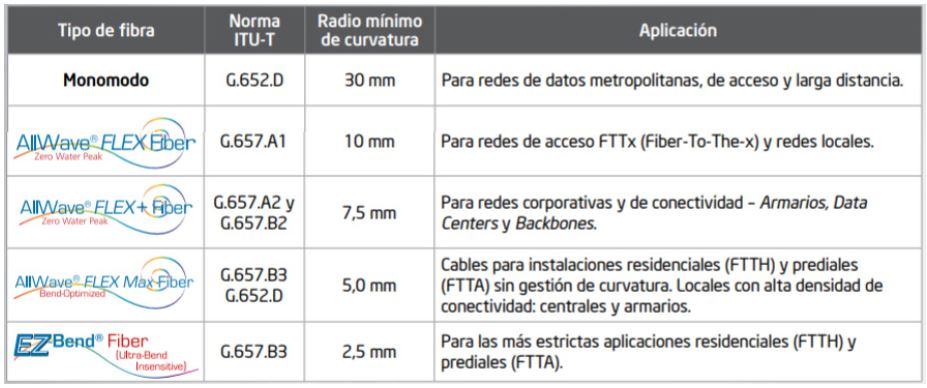
\includegraphics[width = 15cm]{../figuras/Tabla_recomend_Fibras_Furukawa.JPG}
\caption{Tipos de fibra según aplicación. Furukawa.}
\label{Tabla_recomend_Fibras_Frkwa}
\end{figure}

Se selecciona el cable óptico aéreo auto soportado, Mini-Span ADSS\textsuperscript \textregistered \thinspace 424 de AFL bajo la norma ITU-T G.652, descrito como cable dieléctrico mono-modo auto-soportado
de 6 pelos; recomendado para
instalaciones urbanas o rurales aéreas para vanos de hasta 80 metros.

 \medskip

En Fig. \ref{tabla_info_optica_minispanAFL} se especifican los coeficientes de atenuación de la fibra
seleccionada para las diferentes longitudes de onda, necesarios para el
presupuesto de enlace.

\medskip 

\begin{figure} [H]
\centering
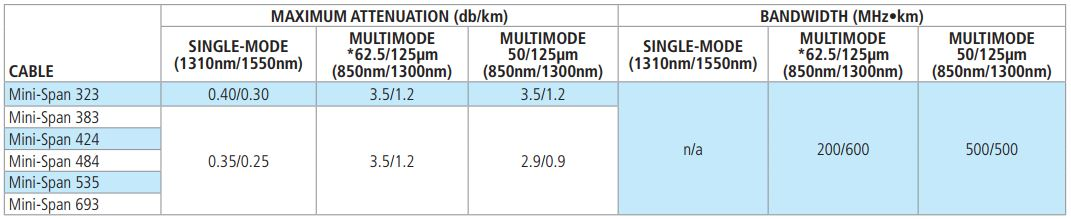
\includegraphics[width = 15cm]{../figuras/Informacion_Optica_MiniSpanAFL.JPG}
\caption{Información Óptica. Hoja de datos Mini-Span\textsuperscript \textregistered \thinspace ADSS Cable, AFL.}
\label{tabla_info_optica_minispanAFL}
\end{figure}

\medskip 

\large
\noindent\textbf{Conectores}
\normalsize
\medskip

En todos los equipos se requieren conectores de tipo SC. Los conectores
SC elegidos del fabricante 3M presentan un coeficiente de atenuación
típico/máximo por inserción de 0.3 dB a 0.6 dB. 

\medskip

\subsubsection{Cálculos de la distancia máxima}\label{subsec_calculo_dist_max_acc}

Se efectúa los cálculos de la distancia máxima entre OLT y ONTs para los
diferentes equipos seleccionados anteriormente. Téngase en cuenta que en
todos los cálculos realizados se utilizan las potencias de transmisión más
bajas para permitir un margen en el enlace.

\medskip

Para calcular la distancia máxima utilizando el presupuesto de enlace, se
despeja la distancia de la ecuación \ref{Ec_Presupuesto_enlaceFibra_Acc}.\medskip

\begin{equation}\label{Ec_Dist_Max_Fibra_Acc}
D\geq \frac{P-[E*P_e+C*P_C+S1+S2+F]}{P_{fo}}
\end{equation}

La ecuación \ref{Ec_Dist_Max_Fibra_Acc} no refleja completamente la distancia máxima, ya que no
tiene en cuenta que la cantidad de empalmes a realizar depende de la
longitud del enlace. Por lo cual, se tiene en cuenta esta relación, resultando
en la Ecuación \ref{Ec_Dist_Max_Fibra2_Acc}.

\begin{equation}\label{Ec_Dist_Max_Fibra2_Acc}
D\geq \frac{P-[C*P_C+S1+S2+F]}{E*A_e+P_{fo}}
\end{equation}

Con el fin de comparar las distancias máximas entre OLT y ONTs
dependiendo los equipos seleccionados y utilizando la Ecuación \ref{Ec_Dist_Max_Fibra2_Acc}, se
conformó Fig. \ref{Tabla_DisMax_ONT_OLT_Acc} con las diferentes distancias máxima según el equipo
elegido, y si se calculó desde ONT a OLT (Upstream) y desde OLT a ONT
(Downstream). \medskip

Cabe destacar que se utilizan las pérdidas de la fibra óptica de marca Furukawa (mayores), dado que de esta manera el diseño contempla un futuro cambio de proveedor. \medskip

Valores fijos a tener en cuenta:\medskip

\begin{itemize}

\item Pérdida en Fibra óptica:
	\begin{itemize}
 		\item[$\circ$] 0.4 dB/km en 1310 nm (Upstream)
		\item[$\circ$] 0.35 dB/km en 1490 nm (Downstream)
    \end{itemize}
\item Cantidad de conectores: 2 conectores
\item Pérdidas por conectores: 0.6 dB para conectores SC
\item Perdidas por splitters: 0 dB (no se consideran en este caso)
\item Factor de proyecto: 0 dB (no es un valor relevante para el tipo de
análisis que se realiza en esta ocasión).
\item E: 0.25 empalmes/km. (Teniendo en cuenta que el rollo de fibra
óptica es de unos 4 km)
\item $A_e$: 0.1 dB/empalme.
\end{itemize}




\begin{figure} [H]
\centering
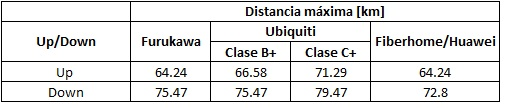
\includegraphics[width = 12 cm]{../figuras/DistMaxONT_OLT_acc.jpg}
\caption{Distancias máximas correspondientes a cada conjunto OLT/ONT}
\label{Tabla_DisMax_ONT_OLT_Acc}
\end{figure}

\medskip

En Fig. \ref{Tabla_DisMax_ONT_OLT_Acc} es posible notar la
cercanía entre las diferentes distancias. Como se ha comentado anteriormente, el
transceptor de Clase C de Ubiquiti al tener mejores prestaciones permitiría
una distancia mayor, aunque con la distancia máxima que demuestran los
otros equipos ya se está dentro de norma, que es justamente lo que se busca
demostrar. 

\medskip

Se decide utilizar la OLT de Fiberhome y ONT de Huawei dado que cumplen con las características requeridas, es una combinación de equipos que se utiliza en el mercado (la utiliza BVC) y su costo es considerablemente menor a los demás equipos analizados. En subsección \label{Colocar_seccion_costo_de_red} se detallan los precios. 

\subsection{Topología de red}

En la subsección \ref{sub_preSelecEq_fibra_acc} se ha justificado la elección del equipo OLT de Fiberhome, que permite brindar servicio hasta 1024 ONTs. Según el estudio demográfico y
socioeconómico realizado en el capítulo \ref{CAP_ANALISIS_DEMOGRAF}, se estima un total de 113 potenciales abonados. En consecuencia, se dimensiona la red para la conexión de 128 ONTs (4
splitters 1:32). De esta manera se cubre la cantidad de abonados estimada,
dejando un margen de 15 ONTs (disponibilidad extra del 11.7\%) y se
utilizan 4 puertos GPON del OLT.\medskip

Dado que se prevé una penetración del 60\% en el mercado, se tiene en cuenta dicho porcentaje de abonados (el 60\% de viviendas en cada zona).\medskip

Es necesario aclarar que el 60\% del total de viviendas expuestas en Fig. \ref{Fig_Division_zonas_Nogoli} no es 113, sino que da como resultado 122. Esto no debe ser motivo de
confusión, ya que se ha llegado al estimado de 113 abonados teniendo en
cuenta censos y factores socioeconómicos (p. ej. descartando hogares con
NBI\footnote{Necesidades Básicas Insatisfechas}) mientras que la división por zonas es una aproximación de la cantidad de viviendas y su distribución en la región, para el diseño y
dimensionamiento de la red.\medskip

Se decide la implementación de una red GPON FTTH con una topología
física tipo árbol y con 1 (un) nivel de splitter. Se define dicha topología ya
que permite una fácil implementación, un bajo costo (en comparación con
otras topologías, como anillo por ejemplo), y permite cierto grado de
robustez (en comparación con topología en tipo bus) al descentralizar la red
con la implementación de jerarquías y ramificaciones. No se considera
justificable la inversión requerida para la implementación de redundancia en
la red, dadas las condiciones demográficas y poblacionales de la localidad.\medskip

En Fig. \ref{fig_Topologia_Arbol_acc} se expone un esquema simplificado de la topología física y lógica utilizada.

\begin{figure}[H]
\centering
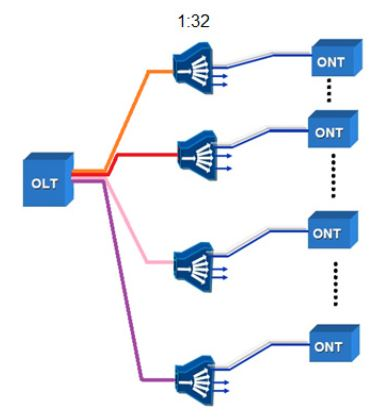
\includegraphics[width = 8 cm]{../figuras/Topologia_Arbol.jpg}
\caption{Topología tipo árbol.}
\label{fig_Topologia_Arbol_acc}
\end{figure} \medskip

Cabe destacar que la topología física y la lógica no presentan diferencias en
la red diseñada. (Ver Fig. \ref{fig_disposicion_equipos_acc}). 

\medskip

Con base en lo mencionado anteriormente y aprovechando las
características demográficas de la zona, se decide la disposición de OLT,
Splitters y ONTs que se expone en Fig. \ref{fig_disposicion_equipos_acc}.


\begin{figure}[H]
\centering
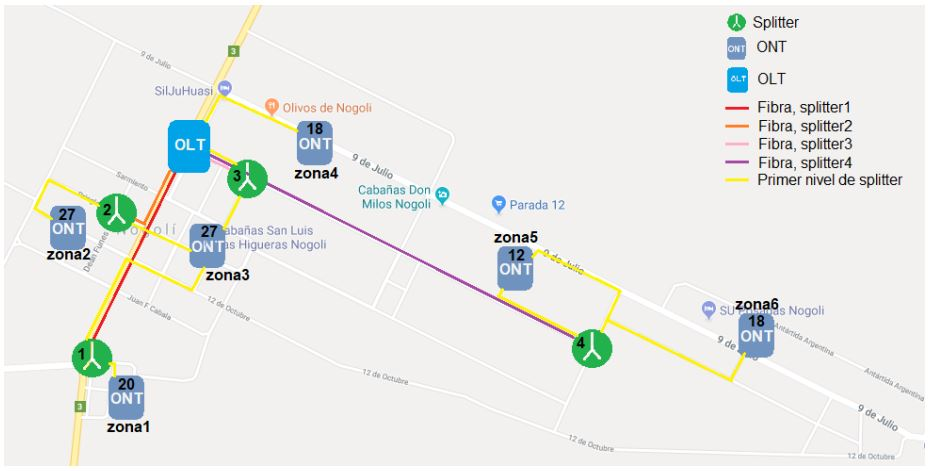
\includegraphics[width = 15 cm]{../figuras/OLTs_ONTs_Split_disposicion.jpg}
\caption{Disposición de OLT, Splitters y ONTs.}
\label{fig_disposicion_equipos_acc}
\end{figure} 

\medskip

La disposición de los splitters se define en función de la cantidad de
viviendas por zona. La OLT se ubica en una zona céntrica para facilitar su
mantenimiento, así mismo se busca su ubicación lo más equidistante
posible de los splitters para brindar una cierta uniformidad a la red. Cabe
destacar que se ha colocado un ONT por zona en representación de los
demás, indicando en la parte superior del bloque la cantidad de ONTs que
se prevé para cada zona (60\% de las viviendas).

\medskip

Se requiere utilizar cajas de distribución óptica aéreas para la contención de los splitters. La característica que deben cumplir es admitir la cantidad de fibras requeridas para utilizar splitters 1:32. En la sección \label{Colocar_sec_costo_red} se analizan los precios y en base a la disponibilidad en le mercado se elige el equipo mas conveniente.

\medskip

Se debe utilizar una caja de empalme terminal (NID\footnote{Network Interface Device.}) para implementar la
interface entre la fibra de distribución y la fibra de acometida (drop). 
La instalación de los equipos NID se realiza en los
postes de baja tensión, circundantes a los abonados. Por consiguiente, la
distancia entre los mismos y las viviendas es como máximo de 10 metros.
Esto implica que la longitud máxima del cable de acometida es de 10 m
aproximadamente, dato que se utiliza en el cálculo de presupuesto óptico
de potencia.

\medskip

Siguiendo la recomendación de la Fig. \ref{Tabla_recomend_Fibras_Frkwa}, para la fibra de acometida, se utiliza fibra óptica bajo la norma ITU-T G.657.

\medskip

Analizando las soluciones de redes FTTH de la empresa Tecnored S.A.\footnote{www.tecnored.com.ar (11/6/2018)},
se utiliza Cable Drop compacto metálico Low Friction, especialmente
desarrollado para instalaciones de acceso final al abonado (tipo drop) en
redes FTTH y FTTA. Los elementos de tracción en hilos de acero posibilitan
la instalación del cable en ducto por tracción o empuje, sin la utilización de
una guía de instalación.\footnote{Fuente: Especificación técnica 2499-V26 – Furukawa (30/05/2016)} En la Fig. \ref{fig_SeccionCableDrop} puede verse la sección transversal del cable elegido.

\medskip

\begin{figure} [H]
\centering
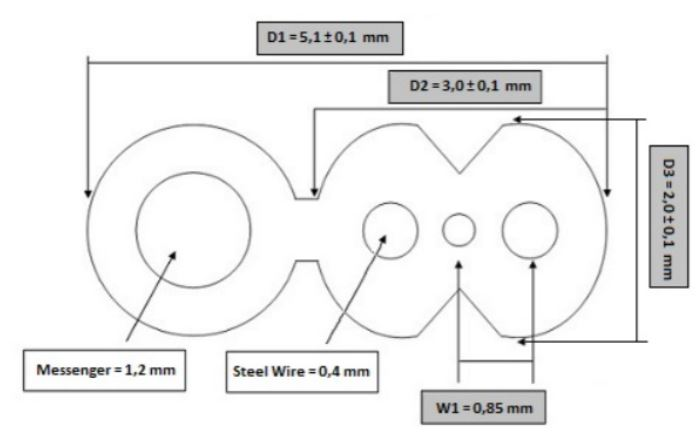
\includegraphics[width = 10 cm]{../figuras/Seccion_cable_drop.jpg}
\caption{Sección transversal cable drop.}
\label{fig_SeccionCableDrop}
\end{figure}

\medskip

A continuación, en la tabla \ref{Tabla_distanciasOLT-ONT}, se exponen las longitudes de las fibras desde
OLT hasta los Splitters, así como el máximo recorrido de fibra hasta ONTs.

\medskip

\begin{table} [H]
\centering
\begin{tabular}{|c|c|}
\hline 
\textbf{Fibra} & \textbf{Longitud [m]} \\ 
\hline 
Roja & 690 \\ 
\hline 
Naranja & 340 \\ 
\hline 
Rosa & 200 \\ 
\hline 
Violeta & 1300 \\ 
\hline 
Mayor recorrido & 2500 \\ 
\hline 
\end{tabular} 
\caption{Longitudes de las fibras desde OLT hasta Splitters}
\label{Tabla_distanciasOLT-ONT}
\end{table}

\medskip

\noindent \textbf{Splitter 1:}
\begin{itemize}
\item Brinda servicio a zona 1 (20 ONTs).
\item 12 fibras libres para brindar servicio a zona 3.
\end{itemize}

\noindent \textbf{Splitter 2:}
\begin{itemize}
\item Brinda servicio a zona 2 (27 ONTs).
\item 5 fibras libres para brindar servicio a zona 3.
\end{itemize}

\noindent \textbf{Splitter 3:}
\begin{itemize}
\item Entre splitter 1 y 2 cubren 17 ONTs de zona 3, por lo tanto splitter 3
brinda servicio a 10 ONTs de zona 3.
\item Con los 22 restantes brinda servicio a zona 4 (18 ONTs).
\end{itemize}

\noindent \textbf{Slplitter 4:}
\begin{itemize}
\item Brinda servicio a zona 5 (12 ONTs) y a zona 6 (18 ONTs).
\end{itemize}

\medskip

En caso de un crecimiento del mercado más allá de lo previsto, la topología
utilizada permite el agregado de un segundo nivel de splitter (bajo la norma
ITU-T. 984.1) aumentando la cantidad de ONTs (recordar que el máximo es
1024 para la OLT elegida). Otra opción viable es el cambio de uno o más
splitters por uno de mayor relación de división (1:64). Llegado el caso, se
deberá analizar el crecimiento y decidir qué solución es conveniente.

\medskip

Aprovechando los tendidos eléctricos de baja tensión, y teniendo en cuenta
la reducida cantidad de viviendas por unidad de área (ver Fig. \ref{Fig_Division_zonas_Nogoli}) se decide utilizar canalización aérea para la implementación de toda
la red. Esto es posible dada la cantidad acotada de fibras requeridas\footnote{En una zona densamente urbana, posiblemente se requiera una canalización
terrestre, dada la imposibilidad de colocar una gran cantidad de fibras en el tendido
eléctrico (debido a la fuerza que ejercen sobre los postes).}.

\medskip

\subsection{Costos de red}\label{Subsec_Costo_Red_Acc}

\medskip

Para la implementación de la red de acceso con FTTH-GPON se requiere de 1 equipo OLT Fiberhome AN5516-04S, 4 splitters con sus respectivas cajas de distribución óptica aéreas, 3000 m de fibra mono-modo Mini-Span ADSS 424 (18.6\% de margen de seguridad) para conexión entre OLT y splitters, 10000 m de la misma fibra para la conexión entre splitters y cajas de distribución\footnote{Se propone 10 km de fibra como una cantidad inicial. Se debe ir reponiendo stock a medida que se requiera.}, 10 cajas de terminación NID (en principio), 500 m de fibra de acometida ITU-T G.657 de la marca Lifefiber\footnote{Sujeto a cambios dependiendo de la disponibilidad en el mercado.} y 113 ONTs Huawei HG8245u\footnote{Se prevé una penetración del 60\% del mercado (113 abonados).} con entrega en comodato. Se propone la tercerización de la instalación de la fibra óptica. 

\medskip

En Tabla \ref{tabla_preciosEquipos_fibra_acc} se expone un presupuesto estimado de los equipos antes mencionados.

\medskip

\begin{table} [H]
\centering
\begin{tabular}{|c|c|c|c|c|}
\hline 
Producto & Cantidad & Precio & Total Parcial & Referencia \\ 
\hline 
OLT Fiberhome AN5516-04S & 1 & 2250 USD & 2250 USD & \ref{cost_OLT_acc}\\ 
\hline 
ONT HUAWEI HG8245u & 113 & 50 USD & 5650 USD & \ref{cost_ONT_acc}\\ 
\hline 
Fibra Mini-Span ADSS 424 & 13000 m & 2.65 USD /m & 34450 USD & \ref{cost_fibraGpon_acc}\\ 
\hline 
Fibra G.657 Lifefiber & 500 m & 1.88 USD & 940 USD & \ref{cost_drop_acc}\\
\hline
Spltter PLCS 1:32 & 4 & 98 USD & 392 USD & \ref{cos_splittGpon_acc}\\ 
\hline
Domo de distribución PLP Coyote & 4 & 228 USD & 912 USD & \ref{cost_Domo_acc}\\
\hline
Caja de terminación NID & 10 & 26 USD & 260 USD & \ref{cost_NID_acc}\\
\hline 
\end{tabular} 
\caption{Precio de los equipos a utilizar en la red de acceso.}
\label{tabla_preciosEquipos_fibra_acc}
\end{table}

\subsubsection{Referencias de precios}
\begin{enumerate}
\item \label{cost_OLT_acc} 
\url{ https://www.ebay.com/itm/new-version-Fiberhome-AN5516-04-GPON-EPON-OLT-
equipment-with-one-8-PON-card-/332035503409?_ul=AR} 
\item \label{cost_ONT_acc}
\url{ https://articulo.mercadolibre.com.ar/MLA-745773121-equipos-ont-huawei-
hg8245u-4ge-2-telefonia-wifi-_JM}
\item  \label{cost_fibraGpon_acc}
\url{ https://www.fiberoptics4sale.com/products/ae-00696c520-aa4}
\item \label{cost_drop_acc}
\url{ https://www.fiberoptics4sale.com/products/clearcurvezbl}
\item  \label{cos_splittGpon_acc}
\url{ https://www.fiberoptics4sale.com/products/f1-plc-32-sca}
\item \label{cost_Domo_acc}
\url{ https://www.fiberoptics4sale.com/products/8006945}
\item \label{cost_NID_acc}
\url{ https://www.fiberoptics4sale.com/products/f1-wm8c}
\end{enumerate}


\chapter{Plan de acción}

En principio se debe hacer mención de como se realizará la instalación de los enlaces troncales y de acceso; para luego analizar cuales son los problemas que pueden presentarse, como advertirlos y la manera de corregirlos. Es decir, para corregirlos se debe tener personal capacitado que se encargue de los inconvenientes, brindándoles los pasos y recomendaciones necesarias para el trabajo encomendado.


\section{Instalación inicial}

A continuación, se hace mención de los pasos a seguir para efectuar la instalación de los enlaces diseñados en las secciones anteriores, teniendo en cuenta la logística y tiempos necesarios.

\subsection{Red de transporte}
En la sección %\ref{transporte}
se dispuso realizar la red de transporte con radio enlaces, los cuales se conforman por 4 equipos y 3 torres. La empresa encargada de colocar las torres, en los 3 puntos, requiere de un tiempo de 1 semana según lo pactado.

\medskip

Una vez instaladas las torres, se comienza por la construcción de un cuarto de equipos en la Localidad de Nogolí, necesario para luego instalar la red de acceso. En el caso de la ubicación de los equipos de respaldo en la localidad de Villa de la Quebrada y en la ubicación del repetidor, se hará uso de racks de exteriores, ver Fig. \ref{fig_rack_ext_plan}, que proporcionen a los equipos de un ambiente óptimo para su funcionamiento. Se predisponen intervalos de mantenimiento, para comprobar la limpieza de los racks mencionados.

\begin{figure} [H]
\centering
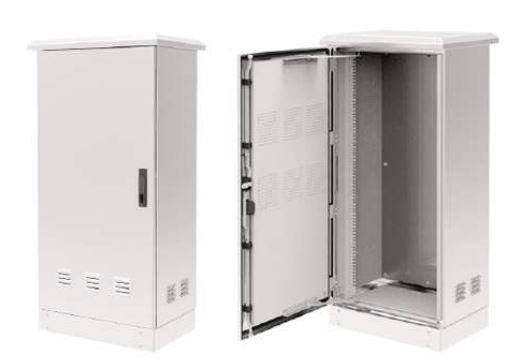
\includegraphics[width= 8 cm]{../figuras/rack_exterior.jpg}
\caption{Rack exterior, especial para telecomunicaciones.}
\label{fig_rack_ext_plan}
\end{figure}

\medskip

De la instalación de los dispositivos en las torres, se hará cargo un equipo de 2 técnicos de planta permanente, que luego se dispondrán para dar servicio técnico en la Localidad de Nogolí, y de el enlace entre el repetidor y la localidad mencionada.

\bigskip

\noindent Los técnicos requerirán de los siguientes parámetros del enlace, resultado de las simulaciones, para la instalación física de los equipos en cada punto del enlace.

\medskip

\noindent\textbf{Enlace Nogolí-Repetidor}
\begin{itemize}
\item \textbf{Altura antena Nogolí:} 5 metros.
\item \textbf{Azimut antena Nogolí:} 258.51º.
\item \textbf{Elevación antena Nogolí:} -1.041º.
\item \textbf{Altura antena Repetidor:} 5 metros.
\item \textbf{Azimut antena Repetidor:} 78.54º.
\item \textbf{Elevación antena Repetidor:} 0.996º.
\end{itemize}

\bigskip

\noindent\textbf{Enlace Villa de la Quebrada-Repetidor}
\begin{itemize}
\item \textbf{Altura antena Villa de la Quebrada:} 12 metros.
\item \textbf{Azimut antena Villa de la Quebrada:} 321.01º.
\item \textbf{Elevación antena Villa de la Quebrada:} -0.520º.
\item \textbf{Altura antena Repetidor:} 5 metros.
\item \textbf{Azimut antena Repetidor:} 141.06º.
\item \textbf{Elevación antena Repetidor:} 0.399º.
\end{itemize}

\subsection{Red de Acceso}
Teniendo en cuenta el diseño de la red en la Sección \ref{sec_radio_enlace_acc}, la instalación consta de la construcción de un cuarto de equipos, el tendido de fibra óptica en postes de baja tensión, instalación de estaciones base, conexión y configuración de equipos en el cuarto ya terminado. No se considera parte de la instalación inicial la conexión de los access point de los clientes.

Se contrata un maestro mayor de obra para la construcción del cuarto de equipos de 4mx4m en el mismo terreno donde se dispone la construcción de la torre de 6 metros. Este cuarto será utilizado para albergar los equipos que conectan la red de transporte con la red de acceso, brindando servicio a cada una de las estaciones base.

Se terceriza con una empresa el tendido de fibra óptica, a quien se le brinda la ubicación geográfica del tendido de la fibra para que diseñe su plan de acción.

La instalación de las estaciones bases corre por cuenta de empleados de planta permanente, a los cuales se les indica la ubicación en la Fig. \ref{fig_redDistribucion_acceso} y una altura de 8 metros, teniendo en cuenta que se colocan sobre el alumbrado público.

\section{Diagrama de Gantt}
El diagrama de Gantt es una herramienta gráfica cuyo objetivo es exponer el tiempo de dedicación previsto para diferentes tareas o actividades a lo largo de un tiempo total determinado \footnote{\url{https://es.wikipedia.org/wiki/Diagrama_de_Gantt}}.

A modo de organizar las tareas a realizar en el proceso de puesta en marcha del proyecto, se realiza un diagrama de Gantt (ver Tabla \ref{tab_gantt}) teniendo en cuenta las tareas principales, los tiempos de finalización, la dependencia entre ellas y el personal encargado de realizarla.

\begin{table} [H]
\centering
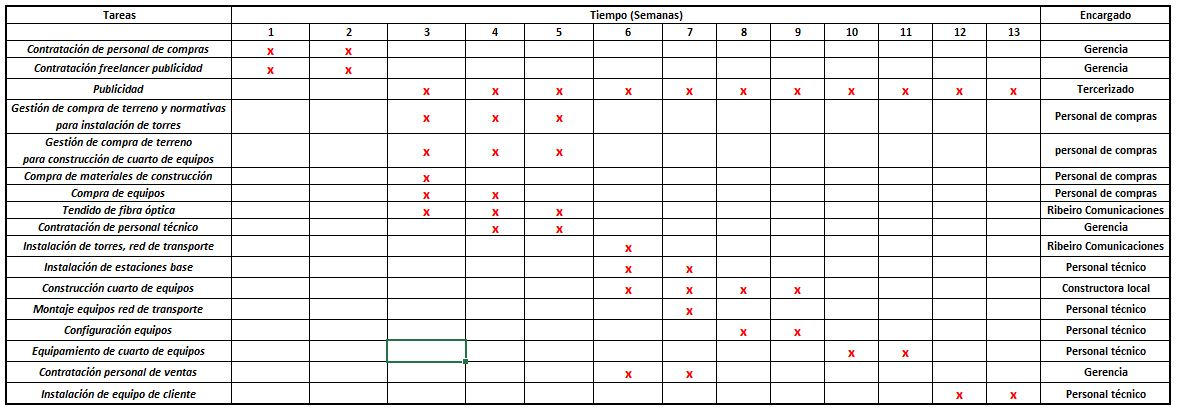
\includegraphics[width= 17 cm]{../figuras/Diagrama_Gantt.jpg}
\caption{Diagrama de Gantt: Puesta en marcha}
\label{tab_gantt}
\end{table}




\section{Personal y equipos requeridos}
Para la óptima instalación de los radio enlaces y la supervisión de los enlaces de fibra óptica se debe tener en cuenta que el personal que se ocupe de esta labor esté completamente capacitado para ello, por esta razón debe cumplir con los siguientes requisitos y la empresa dotarlo de todos los materiales necesarios para tal fin.

El equipo encargado de la instalación de la fibra óptica depende de otra empresa que cuenta con el perfil de personal necesario para esta tarea, por lo cual los requisitos de estos traspasan de este análisis.

\subsection{Perfil de personal}\label{subsec_personal}
El personal efectivo debe cumplir con lo siguientes requisitos.

\begin{itemize}
\item Conocimiento y experiencia en instalación de equipos de radio enlace.
\item Experiencia en reparación de equipos de radio enlace.
\item Conocimiento en redes LAN y WAN.
\item Configuración avanzada de Router.
\item Conocimiento en conectores, cables eléctricos y de datos.
\item Capacitado en trabajos con riesgo eléctrico.
\item Capacitado en trabajo en alturas
\item Conocimiento básico de fibra óptica.
\item Manejo de herramientas de mano.
\end{itemize}

\subsection{Equipos requeridos}
\begin{itemize}
\item Multímetro
\item GPS
\item Analizador de redes digitales
\item Vehículo todo terreno
\end{itemize}

\subsection{Herramientas básicas requeridas}
\begin{itemize}
\item Linterna
\item Brocha
\item Nivel 
\item Llave expansiva
\item Extensión eléctrica
\item Destornillador plano y punta estrella
\item Soldador de estaño 60W (cautín)
\item Pinza de punta
\item Pelacable
\item Alicate
\item Crimpeadora mini coaxial
\item Crimpeadora RJ45
\item Probador de cable utp
\item Martillo
\item Taladro
\item Juego de mechas y brocas
\item Segueta
\item Juego de llaves torx
\item Juevo de llave hexagonales
\item Bisturí
\end{itemize}

\subsection{Equipo para trabajo en alturas}
\begin{itemize}
\item Casco de seguridad
\item Arnés cuerpo completo
\item Eslinga de posicionamiento
\item Eslinga de absorción
\item Arrestador con mosquetón
\item Manila
\item Polea
\end{itemize}


\section{Costos de puesta en marcha}
A modo de explicar detalladamente las tareas a realizar para la puesta en marcha del proyecto, se lista y explica cada una de ellas, y luego en la Tabla \ref{tab_costo_puesta_marcha}, se menciona cada costo que conforman la inversión inicial.

\subsection{Publicidad}
Se decide comenzar con la publicidad en paralelo a la puesta en marcha de la obra para tener una mejor llegada, con un mayor rango de tiempo, al mercado potencial. Para esta actividad se destina un monto de 500 USD.

Haciendo uso de las páginas Freelancer y/o Workana, se le destina a teletrabajadores \footnote{El teletrabajo, o trabajo a distancia, permite trabajar en un lugar diferente a la oficina. El trabajo se realiza en un lugar alejado de las oficinas centrales o de las instalaciones de producción, mediante la utilización de las nuevas tecnologías de la información y la comunicación.} la ejecución de un plan de publicidad masiva en redes sociales, teniendo un tiempo estimado de 10 semanas, como se menciona en el Capítulo \ref{cap_plan_de_negocios}.
 
\subsection{Gestión de compra}

El personal de compras se deberá encargar de las tareas que se mencionan a continuación.

\medskip 

En la tarea \textbf{Gestión de compra de terrenos y normativa para instalación de torres}, se contempla el tiempo requerido (3 semanas) por el personal de compras para la adquisición de terrenos y el estudio de la normativas vigentes para la instalación de las torres. Además, el personal debe encargarse de alquilar los palos de baja tensión a la empresa EDESAL, para el tendido de la Fibra Optica (interconexión de estaciones base) que forma parte de la red de acceso.

Se realiza la \textbf{Gestión de compra de terrenos para la construcción del cuarto de equipos} en la Localidad de Nogolí, en paralelo a la tarea antes mencionada.


\subsection{Compra de materiales de construcción}
Pasada la segunda semana desde la puesta en marcha de la obra, se realiza la compra de los materiales de construcción del cuarto de equipos y también las mallas olímpicas perímetrales necesarias para resguardar la seguridad de los equipos e infraestructura. En la Tabla \ref{tab_costo_puesta_marcha}, se listan los costos de los materiales antes mencionados.

\subsection{Compra de equipos}
Se destinan la tercer y cuarta semana a la compra de los equipos de la red de transporte y la red de acceso, detallados en las Tablas \ref{tabla_precios_transp} y \ref{tabla_preciosEquipos}

\subsection{Tendido de fibra óptica}
El tendido de fibra óptica en la red de acceso se terceriza con la empresa Ribeiro Comunicaciones, destintando tres semanas para tal fin.

\subsection{Contratación de personal técnico}
Se plantea contratar el personal técnico durante la cuarta y quinta semana, ya que esto permite reducir gastos de salario al no mantener personal ocioso. El lector puede observar que el personal técnico comienza a operar en la sexta semana con la instalación de las estaciones base.

\subsection{Instalación de estaciones base}
Una vez contratado el personal técnico, se realiza la instalación de las estaciones base. Se destaca que el sector de gerencia indica de forma precisa al personal técnico la ubicación y altura exactas de las estaciones base.

\subsection{Construcción cuarto de equipos}
Se contrata a una constructora local para la construcción del cuarto de equipos. Esta tarea comienza junto con la instalación de las torres.

\subsection{Montaje equipos red de transporte}
Una vez finalizado el montaje de las torres en la red de transporte, se comienza la instalación de los equipos punto a multipunto, rack de exteriores y switches correspondientes. Esta tarea es realizada por el personal técnico y se estima una semana para ser llevada a cabo.

\subsection{Configuración equipos}
Una vez montada la red, tanto de transporte como de acceso, se destinan dos semanas para la configuración de las mismas. Dicha tarea se encuentra a cargo del personal técnico.

\subsection{Equipamiento de cuarto de equipos}
Luego de terminar la construcción del cuarto de equipos, se puede comenzar con la instalación de los dispositivos que alimentan la red de acceso, recordando que también en este punto se encuentra el terminal del enlace punto a punto de la red de transporte. 

Los dispositivos a conectar se encuentran descriptos en el Capítulo \ref{cap_red_acceso}.


\subsection{Contratación personal de ventas}
Para reducir el gasto en sueldos, se espera que concluyan las tareas de instalación de la red de transporte y de las estaciones bases que forman parte de la red de acceso, para realizar la contratación del personal de ventas, para que realicen los contratos necesarios para realizar la instalación de los equipos en la casa de los clientes.

\subsection{Instalación de equipo de clientes}
Luego de las primeras ventas del servicio, se comienza por instalar los equipos terminales en los hogares de los clientes, en la Sección \ref{sec_inst_inicial_plan_accion}.





% Table generated by Excel2LaTeX from sheet 'Hoja2'
\begin{table}[H]
  \centering
    \begin{tabular}{|l|l|l|}
    \hline
    \multicolumn{3}{|c|}{\textbf{Inversion inicial}} \\
    \hline
    \multicolumn{1}{|c|}{\textbf{Descripción}} & \textbf{Costo} & \textbf{Referencia} \\
    \hline
    \multicolumn{3}{|c|}{\textbf{Red de transporte}} \\
    \hline
    Equipos & \multicolumn{1}{r|}{             27.585 USD } & \ref{cost_inv_13} \\
    \hline
    Terreno  Nogolí 20x50 m  & \multicolumn{1}{r|}{             30.000 USD } & \ref{cost_inv_1} \\
    \hline
    Terrenos (Repetidor y villa de la quebrada) & \multicolumn{1}{r|}{             10.000 USD } &  \\
    \hline
    Malla olímpica en terrenos & \multicolumn{1}{r|}{               2.000 USD } &  \\
    \hline
    Instalación Torres & \multicolumn{1}{r|}{               1.000 USD } &  \\
    \hline
    \multicolumn{3}{|c|}{\textbf{Red de acceso}} \\
    \hline
    Equipos & \multicolumn{1}{r|}{             24.164 USD } & \ref{cost_inv_14} \\
    \hline
    Instalación de fibra  6000 m aprox(0,8 USD/m) & \multicolumn{1}{r|}{               4.800 USD } & \ref{cost_inv_2} (Tercerizado BVC)  \\
    \hline
    \multicolumn{3}{|c|}{\textbf{General}} \\
    \hline
    Cuarto de equipos 6x6x2.6 m & \multicolumn{1}{r|}{               3.150 USD } &  \\
    \hline
    Gabinete exteriores & \multicolumn{1}{r|}{                  480 USD } & \ref{cost_inv_3} \\
    \hline
    Kit de herramientas & \multicolumn{1}{r|}{                  220 USD } & \ref{cost_inv_4} \\
    \hline
    Fiat Fiorino & \multicolumn{1}{r|}{               5.300 USD } & \ref{cost_inv_5} \\
    \hline
    Escalera & \multicolumn{1}{r|}{               1.100 USD } & \ref{cost_inv_6} \\
    \hline
    Equipos de seguridad & \multicolumn{1}{r|}{                  780 USD } & \ref{cost_inv_7} \\
    \hline
    Ropa seguridad & \multicolumn{1}{r|}{                  105 USD } & \ref{cost_inv_8} \\
    \hline
    Computadora ofimatica & \multicolumn{1}{r|}{                  260 USD } & \ref{cost_inv_9} \\
    \hline
    Notebook & \multicolumn{1}{r|}{                  315 USD } & \ref{cost_inv_10} \\
    \hline
    Escritorio y silla & \multicolumn{1}{r|}{                  158 USD } & \ref{cost_inv_11} \\
    \hline
    Instalación eléctrica cuarto de equipos & \multicolumn{1}{r|}{                  500 USD } &  \\
    \hline
    Conectores (RJ45, LC, SC) y cable UTP & \multicolumn{1}{r|}{                  500 USD } &  \\
    \hline
    UPS para repetidor & \multicolumn{1}{r|}{                  192 USD } & \ref{cost_inv_12} \\
    \hline
    \textbf{COSTO TOTAL} & \multicolumn{2}{l|}{\textbf{                                                               112.609 USD }} \\
    \hline
    \end{tabular}%
    \caption{Costos de puesta en marcha}
  \label{tab_costo_puesta_marcha}%
\end{table}%


\subsection{Referencias de precios}

\begin{enumerate}
\item \label{cost_inv_13} Tabla \ref{tabla_precios_transp}.
\item \label{cost_inv_1}
\url{https://sanluiscapital.olx.com.ar/vendo-terreno-en-nogoli-excelente-opurtunidad-ideal-para-emprendimiento-turistico-iid-960150457}
\item \label{cost_inv_14} Tabla \ref{tabla_preciosEquipos_fibra_acc}.
\item \label{cost_inv_2}
\url{http://bahiavision.com.ar/}
\item \label{cost_inv_3}
\url{https://articulo.mercadolibre.com.ar/MLA-605891292-gabinete-exterior-poste-metalico-cctv-camara-dvr-seguridad-_JM}
\item \label{cost_inv_4}
\url{https://articulo.mercadolibre.com.ar/MLA-618037010-kit-herramientas-nisuta-reparacion-pc-58-piezas-redes-pinza-_JM}
\item \label{cost_inv_5}
\url{https://auto.mercadolibre.com.ar/MLA-746994169-fiat-fiorino-13-fire-2011-_JM}
\item \label{cost_inv_6}
\url{https://articulo.mercadolibre.com.ar/MLA-701058041-escalera-extensibledielectrica-fibra-de-vidrio-hasta-977-m-_JM}
\item \label{cost_inv_7}
\url{https://articulo.mercadolibre.com.ar/MLA-639056941-kit-silleta-descensor-antipanico-soga-equipo-completo-_JM}
\item \label{cost_inv_8}
\url{https://articulo.mercadolibre.com.ar/MLA-636016136-kit-botin-de-seguridad-camisapantalon-de-trabajo-oferta-_JM}
\item \label{cost_inv_9}
\url{https://articulo.mercadolibre.com.ar/MLA-707571116-pc-escritorio-windows-10-amd-a4-6300-1tb-4gb-ddr3-8470d-_JM}
\item \label{cost_inv_10}
\url{https://articulo.mercadolibre.com.ar/MLA-726631526-notebook-14-lenovo-ideapad-320-14iap-80xq006r-intel-w10-_JM}
\item \label{cost_inv_11}
\url{https://articulo.mercadolibre.com.ar/MLA-615815201-combo-silla-escritorio-biblioteca-armado-sin-cargo-_JM}
\item \label{cost_inv_12}
\url{https://articulo.mercadolibre.com.ar/MLA-625205834-ups-apc-bx800ci-800va-6-t-estabilizador-gtia-2-anos-bx800-_JM}
\end{enumerate}



\section{Instalación al cliente}\label{sec_inst_inicial_plan_accion}
Una vez terminadas las obras para poder brindar servicio Triple play a los habitantes de la Localidad, que hubiesen contratado el servicio, se disponen de otros 2 técnicos capacitados contratados, por aproximadamente 2 semana, ya que se calcula que al iniciar la pre-venta el 40\% del mercado contratará el servicio la primer semana, por lo cual para reducir los tiempos de instalación se disponen 2 cuadrillas de 2 personas que deben cumplir con un mínimo de 4 equipos instalados por día.

\medskip

\noindent Los técnicos encargados de las instalaciones deben asegurarse de seguir los siguientes pasos:

\begin{enumerate}
\item En principio, cuando la cuadrilla llega al domicilio del cliente debe verificar que cuenta con el comprobante entregado por el sector de ventas.
\item Según el diseño realizado en la Sección \ref{sub_analisis_enlace_acc}, el equipo de radio debe colocarse a una altura de aproximadamente 3 metros (ver Fig. \ref{fig_instalacion_nanoloco_accion}, es decir, los técnicos deben evaluar donde la localizarán en el hogar.

\begin{figure}
\centering
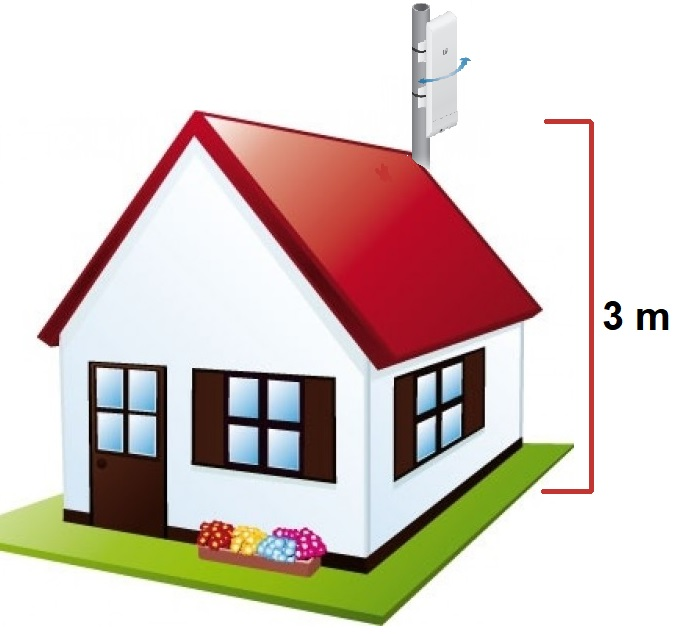
\includegraphics[width= 8 cm]{../figuras/instalacion_nanoLoco.jpg}
\caption{Imagen ilustrativa de la instalación de Nano loco M2.}
\label{fig_instalacion_nanoloco_accion}
\end{figure}

\item Luego de instalar el caño de soporte, deben seguir la guía de instalación provista por Ubiquiti del equipo NanoStation loco M2 \footnote{Quick Start Guide NanoStation loco M2 - Ubiquiti (\url{https://dl.ubnt.com/guides/NanoStation_M/NanoStation_M_Loco_M_QSG.pdf}) - 10/10/18}.
\item Por último, los técnicos deben verificar si los 3 servicios (VoIP, Internet y IPTV) funcionan correctamente, respetando el paquete contratado por el cliente.
\item Una vez realizada la verificación, el cliente debe firmar un acuerdo de aceptación del servicio.
\end{enumerate}

\section{Mantenimiento}
Se entiende por protocolo de revisión de equipos a las acciones de observación, medición, comprobación y análisis de datos técnicos y ambientales, que se toman para definir si un equipo es apto para el desempeño de un muestreo, identificar los impactos inherentes a las actividades del Sector, y conocer su variación a través del tiempo \footnote{\label{note1}Fuente: "Soporte técnico integral de la operación y mantenimiento de las redes de comunicaciones de la empresa SITCOM SAS", Alvaro Alejandro Unigarro Palacios, 2013.}.

\subsection{Mantenimiento preventivo}
El mantenimiento preventivo, como su nombre lo indica, se practica con el propósito de cuidar e inspeccionar los equipos. 

La aplicación del mantenimiento preventivo permite que los equipos funcionen a plena capacidad técnica y elimina los posibles riesgos de quedar fuera de servicio, ocasionando paradas largas por fallas graves, lo cual proporciona grandes riesgos.

Siempre y cuando el \textbf{enlace punto a punto} se encuentre en condiciones normales de funcionamiento, el equipo de trabajo deberá realizar revisiones cada 1 mes del mismo en su totalidad, supervisando y controlando en cada uno de los equipos que forman parte del enlace los siguientes datos:

\begin{itemize}
\item El equipo y elementos que lo soportan deberán estar libres de oxidación, corrosión, soluciones, suciedad, hilachas y depósitos.
\item Las conexiones y conectores, tramos, terminales, puertos de conexión, etc., deben encontrarse en óptimas condiciones. En el momento que se encuentre alguno de los elementos antes mencionados con la posibilidad de falla (oxidación, rotura, desgaste de trabas), se deberá hacer el remplazo.
\item En cada uno de los equipos supervisar las potencias de transmisión y recepción, verificando que se encuentren dentro del rango necesario, para un correcto desempeño.
\item Medir las tensiones de alimentación, como así también comprobar los dispositivos de seguridad si ese fuese el caso. 
\end{itemize}

En el caso del enlace punto a multipunto, el mantenimiento preventivo también debe realizarse mensualmente, comenzando 15 días después de la primer revisión del enlace punto a punto. Se deben revisar los items antes mencionados para red punto a punto, prestando especial atención al tendido de fibra óptica, que provee de servicio a las estaciones bases Rocket M2 Titanium. 

\subsection{Mantenimiento correctivo}

El mantenimiento correctivo, es la acción técnica que se utiliza cuando un equipo e instalación ha dejado de funcionar o lo hace defectuosamente y se tiene que entrar a reparar.
Esto origina cargas de trabajo incontrolables que causan muchas actividades, equipos fuera de uso por largos tiempos, lo cual ocasiona sobre costos por pago de trabajos extras, compra de materiales y repuestos en forma inmediata. En resumen son las consecuencias lógicas cuando se sufre un accidente inesperado.

Como se hace mención en la Sección \ref{subsec_personal}, los técnicos están capacitados para las reparaciones de las estaciones bases, como así también los equipos de enlace punto a punto utilizados entre la Localidad de Villa de la Quebrada y Nogolí, por lo cual, ante fallas en los equipos e instalaciones, los mencionados se harán cargo de las reparaciones, utilizando un sistema de turnos de guardia entre los empleados. 

Para las fallas en el tendido de fibra óptica, el equipo encargado de las reparaciones será el mismo que realiza el tendido de FO en los palos de baja tensión dentro de la localidad de Nogolí. Se considera innecesario contratar personal efectivo para posibles reparaciones de fibra óptica, ya que al analizar tanto la red de transporte como la de acceso, la probabilidad de falla de la fibra óptica en relación a la de los demás equipos que conforman las redes es pequeña.



\chapter{Plan de negocios}\label{cap_plan_de_negocios}
A modo de profundizar en los aspectos financieros del proyecto, se realiza un análisis detallado del mercado como así también de la rentabilidad de la inversión, haciendo uso de herramientas como son el VAN y el TIR.

\section{Análisis Foda}\label{sec_analisis_foda_Pnegocio}

\medskip

Análisis FODA es una herramienta de estudio de la situación de una empresa, institución, proyecto o persona, analizando sus características internas (debilidades y fortalezas) y su situación externa (oportunidades y amenazas).\footnote{Fuente \url{https://es.wikipedia.org/wiki/Analisis_DAFO} 10/10/2018}

\medskip

\noindent \textbf{Fortalezas:}
\begin{itemize}
\item[$\circ$] Conocimiento en el tema.
\item[$\circ$] Servicio novedoso para la región.
\end{itemize}

\medskip

\noindent \textbf{Amenazas:}
\begin{itemize}
\item[$\circ$] Futuras inversiones en WIFI 3.0 provisto por gobierno de San Luis.
\item[$\circ$] Cambios en los pronósticos poblacionales.
\item[$\circ$] Economía inestable.
\item[$\circ$] Mercado reducido.
\end{itemize}

\medskip 

\noindent \textbf{Debilidad:}
\begin{itemize}
\item[$\circ$] Poca experiencia en el campo de las telecomunicaciones.
\item[$\circ$] Poco capital inicial.
\end{itemize}

\medskip 

\noindent \textbf{Oportunidad:}
\begin{itemize}
\item[$\circ$] Nicho de mercado no explotado.
\item[$\circ$] Terreno favorable para implementación de radio enlaces.
\end{itemize}

\section{Misión}
Brindar servicio y soporte de telecomunicaciones a nivel regional, acompañando el desarrollo tecnológico de nuestros clientes, con personal capacitado, infraestructura moderna, total compromiso y excelente calidad.


\section{Visión}
Brindar servicio triple play en toda la provincia de San Luis, manteniendose a la vanguardia del desarrollo tecnológico para disponer de un servicio de calidad para los clientes.

\section{Politicas de calidad}
Teniendo en cuenta su Misión, la empresa se compromete mediante la planificación eficiente de los recursos para el desarrollo, entrega y cierre de cada uno sus servicios:

\begin{itemize}
\item Ofrecer servicios de comunicación e información que satisfagan las necesidades de la población.
\item Contar con un equipo humano competente y comprometido con la innovación y el mejoramiento continuo.
\item Brindar un servicio que cumpla con las expectativas de nuestros clientes en oportunidad y calidad.
\item Establecer la identificación y comprensión de las necesidades de nuestros clientes como un generador de mejora continua de nuestros productos y servicios.
\end{itemize}

\section{Análisis de competencia}\label{sec_analisis_competencia_Pnegocio}

\medskip 

Si bien el servicio triple play no es ofrecido en la localidad de Nogolí, existen empresas que brindan servicio de telefonía, Internet y TV satelital.

\medskip 

Se considera como competencia indirecta a las siguientes prestadoras de servicio:
\begin{itemize}
\item[$\bullet$] DirecTV.
\item[$\bullet$] Telefónica.
\item[$\bullet$] Autopista de la Información\footnote{Antenas WIFI 3.0 (5GHz) y WIFI 2.4 GHz}.
\end{itemize}

\noindent \textbf{DirecTV}

\medskip 

La empresa DirecTV ofrece servicio de televisión digital satelital. Se destacan las siguientes características.

\begin{itemize}
\item Precio del servicio elevado.
\item Considerable costo inicial (compra e instalación de antena parabólica).
\item Alta disponibilidad de servicio.
\item Servicios extra de costo elevado.
\end{itemize}

\medskip 

\noindent \textbf{Telefónica}

\medskip 

Analizando la guía oficial de Telefónica 2017 se encuentra que hay 28 usuarios de telefonía fija en la localidad, indicando que un alto porcentaje del mercado no dispone de este servicio.    

\medskip 

\noindent\textbf{Autopista de la Información}

Como se mencionó en la sección \ref{sec_analisis_mercado_dem}, la localidad dispone de 2 antenas WI-FI 3.0 (5 GHz) y 7 antenas WI-FI a 2.4 GHz, con un promedio de 46 usuarios por antena. Esto indica una baja tasa de datos por usuario, culminando en un servicio de baja calidad.

\medskip 

Dado que hay un alto porcentaje de usuarios de la red de internet pública, se plantea brindar al cliente la opción de mantener el equipo ya adquirido (antena y/o equipo CPE\footnote{Customer Premises Equipment o Equipo Local de Cliente}) en lugar de brindarle la NanoStation Loco M2 en carácter de comodato. Esta opción permite, no sólo reducir costos y despliegue de instalación, sino también brindar comodidad al usuario. Así mismo, el equipo debe cumplir con características mínimas\footnote{Igual o mayor tasa de datos; igual o mayor sensibilidad} para no comprometer la calidad del servicio brindado y se debe incluir explícitamente en el contrato que al utilizar un equipo distinto al recomendado, la calidad del servicio (QoS) queda bajo responsabilidad del cliente.  

\medskip 

\section{Estrategia de producto}

Como se describió en el análisis FODA, se busca explotar la ventaja de disponer de una prestación conformada por tres servicios: teléfono, televisión e internet. El servicio triple play es completamente nuevo en la región, por la cual la estregia de producto se basa en dar a conocer la oferta del mismo, esperando que la inovación y la calidad del servicio sean suficientes para despertar la curiosidad de potenciales clientes.

\section{Estrategia de promoción y publicidad}\label{sec_estrategia_publicidad_Pnegocio}

La principal forma de promoción se basará en la prestación de un buen servicio, ya que teniendo en cuenta que se provee triple play en una pequeña localidad, lo clientes satisfechos serán los mejores promotores dentro de sus contactos. Además, se piensa hacer uso de las redes sociales, que hoy en día son un medio masivo de comunicación bien aceptado, creando páginas de Facebook (con un chat abierto a críticas y sugerencias) e  invirtiendo en publicidad en Instagram. 

En la penetración de mercado se busca abarcar parte del mismo con una sólida estrategia de promoción, como son, descuentos en instalación, descuento por pagos trimestrales o anuales.

Entre las alternativas de comercialización se desarrollará una página de Internet, en donde el cliente puede consultar la visión, misión y políticas de calidad de la empresa, como así también conocer el servicio, el precio de los diferentes paquetes y reservar un turno de conexión para evitar tener que realizar grandes procedimientos como en la mayoría de los casos.

Algunos puntos que se tendrán en cuenta para generar un buen concepto de la empresa:

\begin{itemize}
\item Actualizar constantemente la publicidad de la empresa.
\item Cumplir con las fechas de instalación y visitas del servicio técnico.
\item El uso del uniforme es indispensable durante las horas de trabajo de parte de los socios y empleados.
\item Realizar instalaciones de calidad.
\end{itemize}

\noindent\textbf{Factores críticos de éxito}

\begin{itemize}
\item Oposición al cambio de los potenciales clientes.
\item Calidad del servicio, es una importante característica dentro de la prestación, determinante en la estrategia de producto.
\item Mantener un precios competitivo para el mercado potencial.
\end{itemize}


\section{Recursos humanos}\label{sec_recursos_humanos_Pnegocio}

La empresa se compone de las siguientes áreas.

\begin{itemize}
\item Gerencia
\item Publicidad y Marketing
\item Mantenimiento
\item Atención al cliente
\item Contabilidad
\item Asesoría legal
\end{itemize}

\noindent \textbf{Gerencia}

\medskip

Mayor cargo jerárquico de la empresa, encargado de la toma de decisiones corporativas, de inversión y estratégicas entre otras.

\medskip 

\noindent \textbf{Publicidad y Marketing}

\medskip 

Sector de la empresa encargado de la gestión y aplicación de estrategias de marketing y diseño e implementación de publicidad, ver sección \ref{sec_estrategia_publicidad_Pnegocio}. 

\medskip 

Dada la naturaleza del mercado al que se apunta, es de vital importancia contar con un buen equipo de publicidad ya que la competencia utiliza ampliamente este recurso para abarcar la mayor cantidad posible del mercado. 

\medskip 

\noindent \textbf{Mantenimiento}

\medskip 

El área de mantenimiento cuenta con un \textbf{Jefe de mantenimiento} junto con personal capacitado encargado de la instalación de equipos CPE así como de brindar mantenimiento a las estaciones base y al enlace punto a punto entre las localidades de Villa de la Quebrada y Nogolí.

\medskip 

\noindent \textbf{Atención al cliente}

\medskip 

Se propone brindar atención al cliente con personal freelance. Esto implica una gran reducción de costos, ya que no se contrata de forma efectiva al personal, no se requiere de instalaciones (los servicios e infraestructura no corren por cuenta de la empresa), y hay una variedad de empresas dedicadas a tal fin con precios competitivos y personal capacitado.

\medskip 

\noindent \textbf{Contabilidad}

\medskip 

Se requiere de personal en el área de contabilidad para la liquidación de sueldos, contratación de personal, pago de impuestos, y asesoría contable.

\medskip 

\noindent \textbf{Asesoría legal}

Es importante la asesoría legal ya que el área de las telecomunicaciones se encuentra altamente regulado y legislado. Así mismo, no se requiere de personal efectivo para tal fin por lo que se plantea la contratación de una consultora legal (estudio jurídico), de forma esporádica y no de forma permanente.  

\section{Flujo de fondos}

En el análisis de flujo de fondos se detallan los ingresos y egresos esperados en un cierto plazo de tiempo, 3 y 5 años en este caso, con el fin de determinar CAPEX (CAPital EXpenditure) y OPEX (OPerating EXpense), dos valores importantes a la hora de determinar la rentabilidad de un emprendimiento. Cabe destacar que tanto los egresos como ingresos se analizan en dólares, dada la volatibilidad y dependencia del valor intrínseco del peso argentino en relación a esta otra divisa.

\subsection{Ingresos}

Dada la naturaleza de una empresa de servicios de comunicaciones, la única fuente de ingresos que se dispone es el abono mensual por parte del cliente. Como se ha detallado en el Capítulo \ref{cap_demografico}, se prevé una penetración del 60\% del mercado (113 abonados) y a su vez que un 40\% (45 abonados) contrate el servicio en las primeras dos semanas. En tabla \ref{Tabla_preciosServicios_Pnegocio} se exponen los precios establecidos para cada servicio.

\medskip

De acuerdo a la aproximación de la remuneración establecida por habitante (sección \ref{sec_analisis_socioeconomico}), a que solo se dispone del acceso a internet que brinda Autopista de la Información y a los precios que actualmente posee la competencia (DirecTv como único prestador de servicio de TV Digital en la zona),(ver sección \ref{sec_analisis_competencia_Pnegocio}) se establecen los siguientes precios para cada paquete propuesto:


\begin{table}
\centering
\begin{tabular}{|c|c|}
\hline
Servicio Básico & 52.7 USD \\
\hline
Servicio Premium & 65.8 USD \\
\hline
\end{tabular}

\caption{Precios por servicio.}
\label{Tabla_preciosServicios_Pnegocio}
\end{table}


En tabla \ref{Tabla_ingresos_Pnegocio} se exponen los ingresos previstos hasta 5 años, IVA (27\%) incluído.

\begin{table} [H]
\centering
\begin{tabular}{|c|c|c|c|c|}
\hline
1º Año & 2º Año & 3º Año & 4º Año & 5º Año \\
\hline
69978 USD & 99780 USD & 99780 USD & 99780 USD & 99780 USD  \\ 
\hline
\end{tabular}

\caption{Ingresos anuales.}
\label{Tabla_ingresos_Pnegocio}
\end{table}


\subsection{Egresos}

La inversión inicial requerida para la implementación del proyecto es de 100688 USD, ver tabla \ref{tab_costo_marcha_plan_accion}. En tabla \ref{Tabla_egresos_Pnegocio} se exponen los egresos anuales previstos.

\begin{table} [H]
\centering
\begin{tabular}{|c|c|c|c|c|}
\hline
1º Año & 2º Año & 3º Año & 4º Año & 5º Año \\
\hline
46192 USD & 40802 USD & 40802 USD & 40802 USD & 40802 USD \\ 
\hline
\end{tabular}

\caption{Egresos anuales.}
\label{Tabla_egresos_Pnegocio}
\end{table}


\subsection{CAPEX y OPEX}

CAPEX son inversiones de capital que crean beneficios. Un CAPEX se ejecuta cuando un negocio invierte en la compra de un activo fijo o para añadir valor a un activo existente con una vida útil que se extiende más allá del año imponible.\footnote{Fuente \url{https://es.wikipedia.org/wiki/Capex}.} Aquí, el CAPEX es de 100688 USD (inversión inicial). Se destaca que no se prevé un incremento de CAPEX en el corto plazo, ya que se pretende amortizar la inversión. Así mismo, en el marco de la visión de la empresa, se plantea incrementar el CAPEX en el largo plazo (a partir de 5 años) con fines de expansión y crecimiento de la empresa, ampliando el mercado a zonas circundantes. 

\medskip

OPEX es un coste permanente para el funcionamiento de un producto, negocio o sistema. Puede traducirse como gasto de funcionamiento, gastos operativos, o gastos operacionales.\footnote{Fuente \url{https://es.wikipedia.org/wiki/Opex}.} En tabla \ref{Tabla_OPEX_Pnegocio} se exponen los egresos anuales operativos, es decir el OPEX anual, proyectado a 5 años.

\begin{table} [H]
\centering
\begin{tabular}{|c|c|c|c|c|}
\hline
1º Año & 2º Año & 3º Año & 4º Año & 5º Año \\
\hline
19307 USD & 19589 USD & 19589 USD & 19589 USD & 19589 USD \\ 
\hline
\end{tabular}

\caption{OPEX anual.}
\label{Tabla_OPEX_Pnegocio}
\end{table}

\section{Factibilidad financiera}
Para analizar la factibilidad financiera se utilizarán las herramientas correspondientes a este campo, tomando los valores de gastos e inversiones de las hojas de cálculo adjuntadas al presente documento. En este caso solo se analiza con un 60\% del mercado potencia ocupado.
En la siguiente tienen los diferentes ingresos de dinero por año, en un periodo de 3 años y 5 años. 

\subsection{VAN}
El \textbf{Valor Actual Neto}, cuyo acrónimo es VAN, es un procedimiento que permite calcular el calor presente de un determinado número de flujos de caja futuros, originados por una inversión. La metodología consiste en descontar al momento actual (es decir, actualizada mediante una tasa) todos los flujos de caja futuros o en determinar la equivalencia en el tiempo 0 de los flujos de efectivo futuros que genera un proyecto y comparar esta equivalencia con el desembolso inicial \footnote{\url{https://es.wikipedia.org/wiki/Valor_actual_neto}}.

Se calcula con la herramienta VAN la rentabilidad del negocio con una tasa de descuento del 6 \% y 20\%.

La fórmula que nos permite calcular el VAN, puede verse en la Ecuación \ref{ec_van}.

\begin{equation}\label{ec_van}
VAN=\sum_{t=1} ^{n} \frac{V_{t}}{(1+k)^t} - I_{0}
\end{equation}

\noindent donde,

\begin{itemize}
\item $V_t$: Representa los flujos de caja en cada periodo t;
\item $I_0$: es el valor del desembolso inicial de la inversión;
\item $n$: es el número de períodos considerado;
\item $k$ es el tipo de interés (cuando el VAN toma un valor igual a 0, $k$ pasa a llamarse TIR). 
\end{itemize}

Utilizando los datos de inversión inicial, ingresos anuales y egresos anuales  mencionados en la Sección \ref{sec_flujo_fondos} y una calculadora online de VAN \footnote{\url{https://es.calcuworld.com/calculadoras-empresariales/calculadora-van/}}, se calcula con una tasa de descuento del 6\% y del 20\% para 3 años y 5 años.

\subsubsection{VAN a 3 años} \label{subsec_VAN_3}

En la Fig. \ref{fig_VAN_3_tasa6}, se realiza el VAN a 3 años con una tasa de descuento del 6\%. Como puede verse, tiene una rentabilidad aceptable a 3 años, aunque se esté considerando una tasa baja.

\begin{figure} [H]
\centering
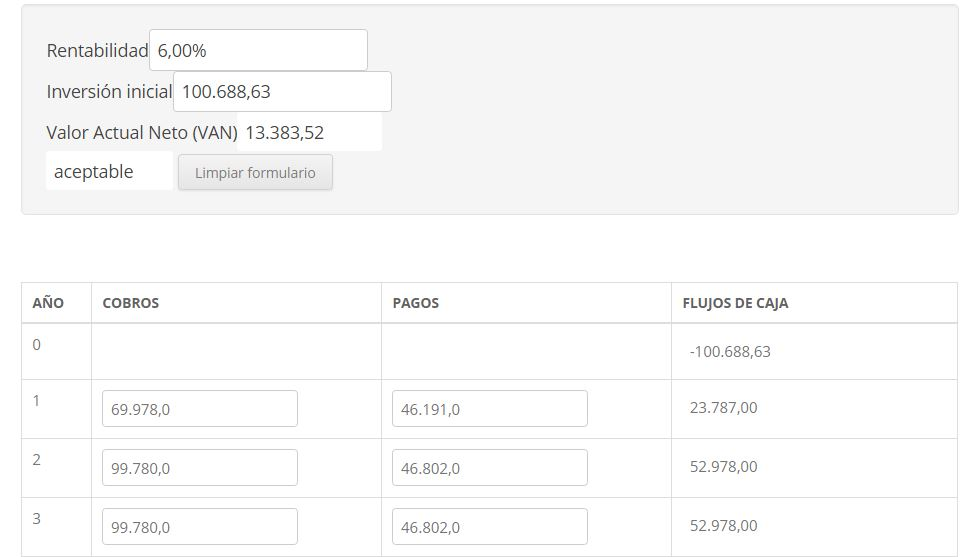
\includegraphics[width= 15 cm]{../figuras/VAN_3anios_6rentabilidad.jpg}
\caption{VAN a 3 años con tasa del 6\%.}
\label{fig_VAN_3_tasa6}
\end{figure}

En la Fig. \ref{fig_VAN_3_tasa20}, se realiza el VAN a 3 años con una tasa del 20\%. En este caso, se tiene un VAN negativo, es decir, con una tasa del 20\% la rentabilidad no es aceptable, siendo desfavorable la inversión en el proyecto.

\begin{figure} [H]
\centering
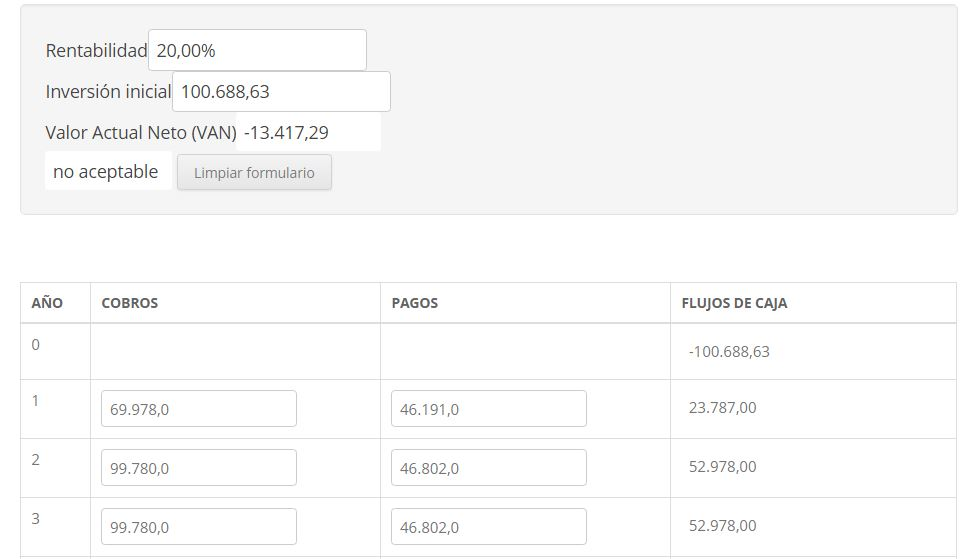
\includegraphics[width= 13 cm]{../figuras/VAN_3anios_20rentabilidad.jpg}
\caption{VAN a 3 años con tasa del 20\%.}
\label{fig_VAN_3_tasa20}
\end{figure}

\subsubsection{VAN a 5 años}

En la Fig. \ref{fig_VAN_5_tasa6} y Fig. \ref{fig_VAN_5_tasa20}, se presentan los resultados del VAN con tasas del 6\% y del 20\%, respectivamente. No es de sorprender que se tenga un mayor VAN, teniendo en cuenta que los ingresos y egresos luego del 3 año, se mantienen.

\begin{figure} [H]
\centering
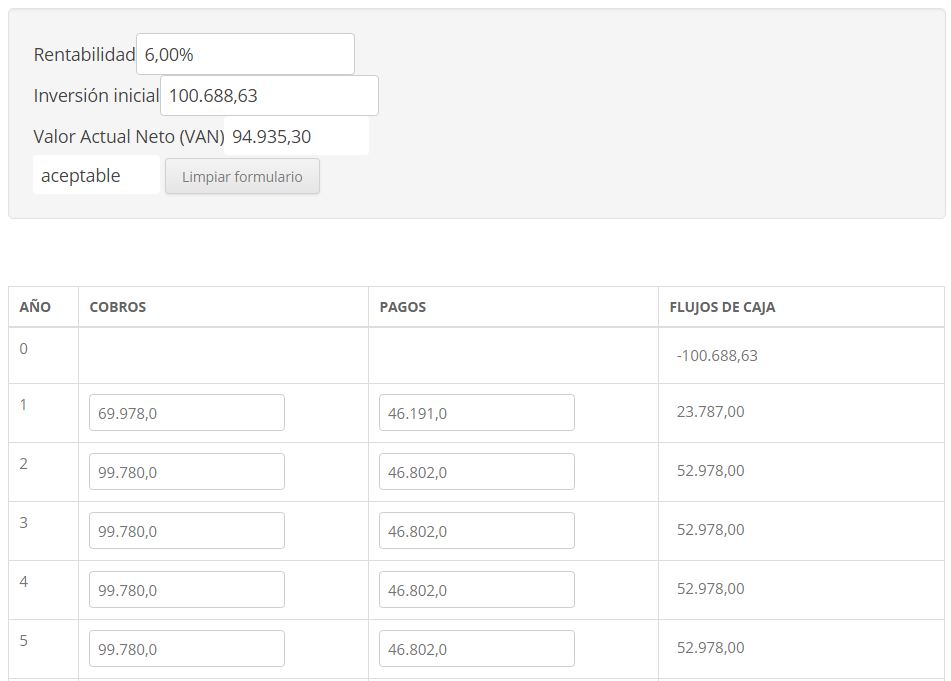
\includegraphics[width= 13 cm]{../figuras/VAN_5anios_6rentabilidad.jpg}
\caption{VAN a 5 años con tasa del 6\%}
\label{fig_VAN_5_tasa6}
\end{figure}

\begin{figure} [H]
\centering
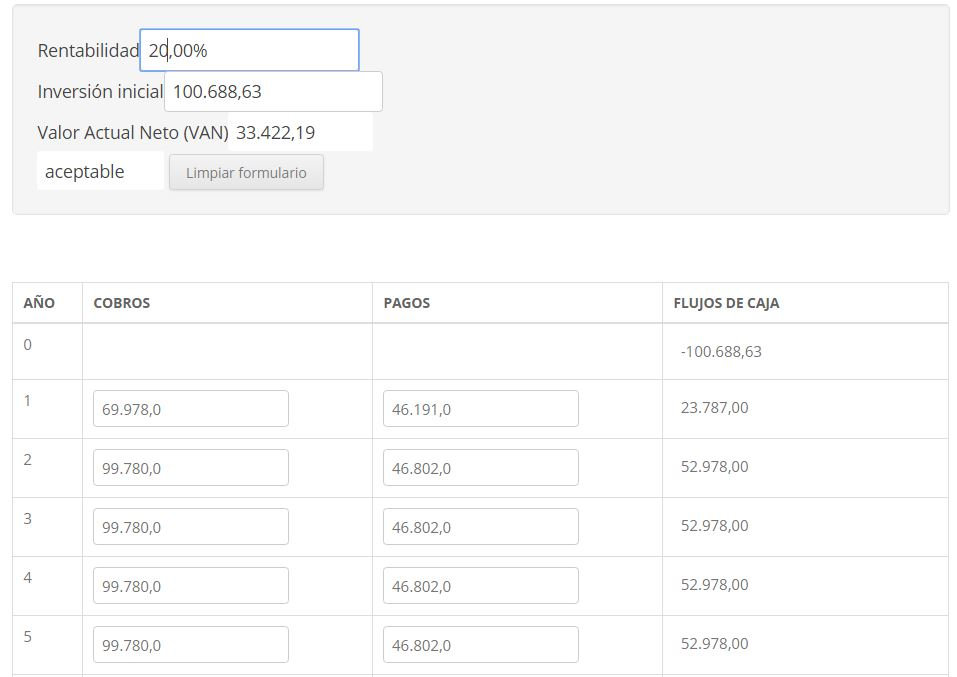
\includegraphics[width= 13 cm]{../figuras/VAN_5anios_20rentabilidad.jpg}
\caption{VAN a 5 años con tasa del 20\%}
\label{fig_VAN_5_tasa20}
\end{figure}
 
\subsection{TIR}
La \textbf{tasa interna de retorno} (TIR), de una inversión es la media geométrica de los rendimientos futuros esperados de dicha inversión, y que implica por cierto el supuesto de una oportunidad para ``reinvertir". En términos simples, diversos autores la conceptualizan como la tasa de descuento con la que el \textbf{VAN} es igual a cero.

Teniendo en cuento la definición de TIR y haciendo uso de la calculadora online \footnote{https://es.calcuworld.com/calculadoras-empresariales/calculadora-tir/}, se obtiene el TIR a 3 años y a 5 años.

En la Fig. \ref{fig_TIR_3}, el TIR a 3 años es de 12.25\%, correspondiendo a lo analizado en la Sección \ref{subsec_VAN_3}, siendo rentable con una tasa del 6\% y no rentable con una tasa del 20\%.

\begin{figure} [H]
\centering
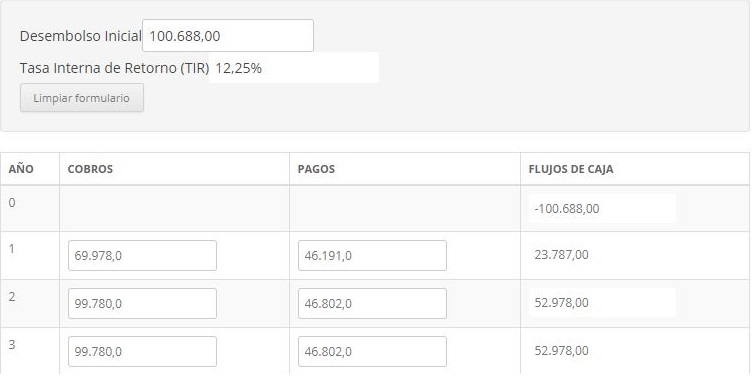
\includegraphics[width= 13 cm]{../figuras/TIR_3anios.jpg}
\caption{TIR a 3 años}
\label{fig_TIR_3}
\end{figure}

En la Fig. \ref{fig_TIR_5}, el TIR a 5 años es de 32.68\% teniendo una rentabilidad interesante, dando un buen pronóstico para la inversión en el proyecto.

\begin{figure} [H]
\centering
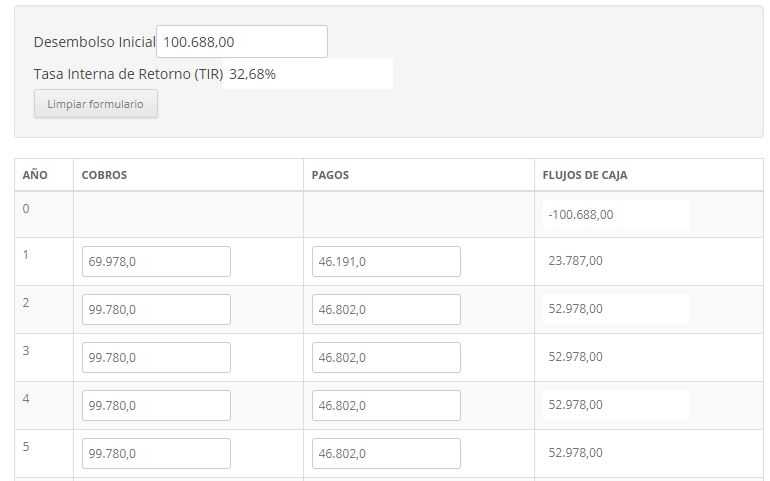
\includegraphics[width= 13 cm]{../figuras/TIR_5anios}
\caption{TIR a 5 años}
\label{fig_TIR_5}
\end{figure}






% --------- ANEXOS ------





\appendix
\clearpage
\addappheadtotoc
\appendixpage

\chapter{Cálculos de enlace de la Red de Transporte} \label{ane_calculo_red_trasporte}
Se proponen 3 enlaces, los cuales se simulan en el programa ``Radio Mobile", a continuación se hace mención de los resultados obtenidos.

\bigskip 

\noindent\textbf{Enlace 1.a:} Villa de la Quebrada (33.018155 S.; 66.289680 O.) y Ruta 146/Acceso Nogolí (32.923676 S.; 66.380755 O.)

\begin{figure} [H]
\centering
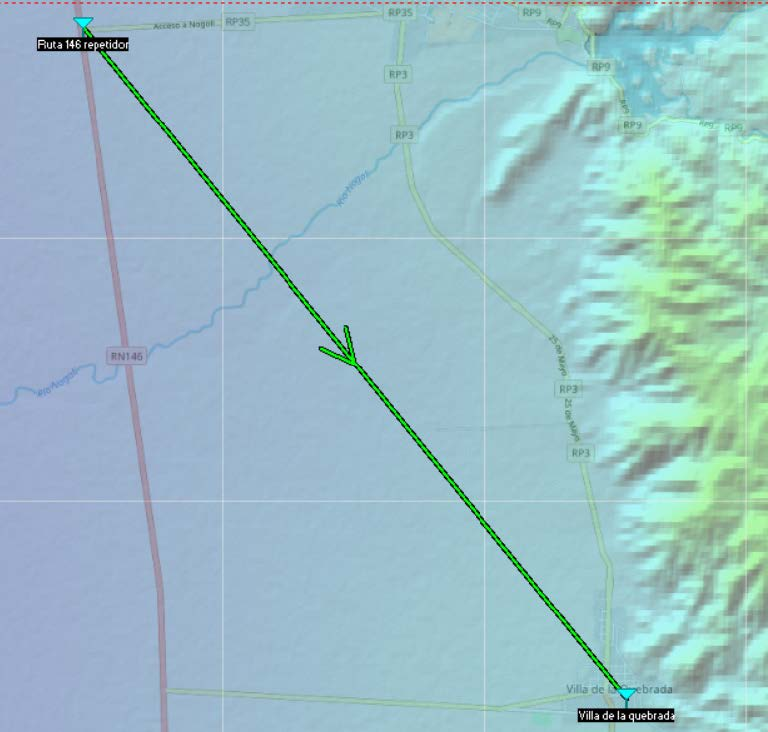
\includegraphics[width= 10 cm]{../figuras/red_transporte_2.jpg}
\caption{Vista satelital Enlace 1.a de Radio Mobile}
\label{fig_red_transporte_2}
\end{figure}

En ambos dispositivos se utiliza la antena de 1 metro de diámetro con una ganancia de 35.3 dBi.

Como puede verse en la Fig. \ref{fig_red_transporte_3}, se obtiene, despejando la primer zona de Fresnel, un Rx relativo de 22 dB, es decir, un enlace robusto.

En la Fig. \ref{fig_red_transporte_3}, las alturas de las antenas Repetidor - Villa de la Quebrada, son de 5 metros y 12 metros, respectivamente. Pero dichas alturas de antenas puede ser variadas entre 4 y 5 metros, en el Repetidor y entre 10 y 12 metros en la Localidad de Villa de la Quebrada.

Se ha decidido ubicar el repetidor en las coordenadas antes mencionadas dado que se dispone de tendido eléctrico para alimentación de equipos, así como línea de vista directa con Nogolí.

\begin{figure} [H]
\centering
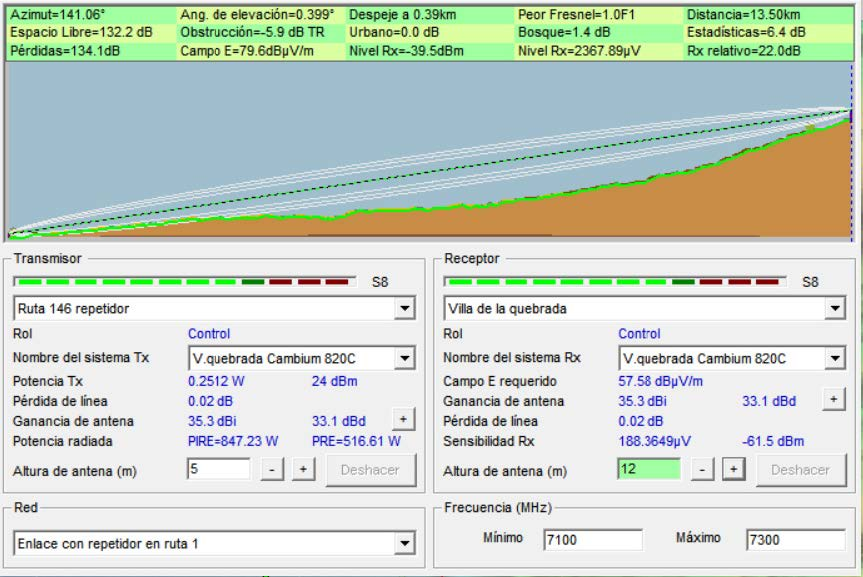
\includegraphics[width= 12 cm]{../figuras/red_transporte_3.jpg}
\caption{Configuración de equipos de Enlace 1.a en Radio Mobile}
\label{fig_red_transporte_3}
\end{figure}

\noindent\textbf{Enlace 1.b}: Nogolí (32.919786 S.; 66.317456 O.) y Ruta 146/Acceso Nogolí (32.923674 S.; 66.380755 O.)

\begin{figure} [H]
\centering
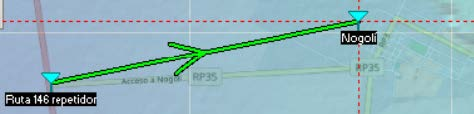
\includegraphics[width= 12 cm]{../figuras/red_transporte_4.jpg}
\caption{Vista satelital Enlace 1.b de Radio Mobile}
\label{fig_red_transporte_4}
\end{figure}

En este caso, como el enlace no presenta grandes dificultades, en ambos dispositivos se utiliza la antena de 0.6 metros de diámetro con una ganancia de 31.1 dBi, permitiendo reducir los costos.

Como puede verse en la Fig. \ref{fig_red_transporte_5}, se obtiene un Rx relativo de 20.5 dB, siendo un enlace robusto aunque en menor medida que el anterior. En este enlace se despeja la primer zona de Fresnel y parte de la segunda, recordando que al despejar al segunda zona de Fresnel la atenuación aumenta.

En la Fig. \ref{fig_red_transporte_5}, las alturas de las antenas Repetidor - Nogolí, son ambas de 5 metros. En este enlace no se presenta la misma flexibilidad que en Villa de la Quebrada con respecto a la altura. Una solución sería remplazar una de las antenas de 0.6 metros por una de 1 metro para tener una mayor ganancia y aumentar el margen de altura.

\begin{figure} [H]
\centering
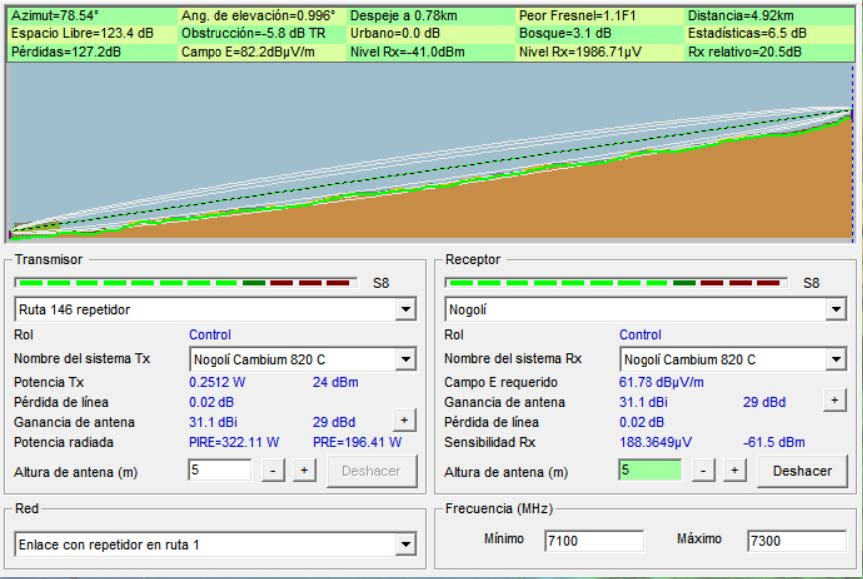
\includegraphics[width= 12 cm]{../figuras/red_transporte_5.jpg}
\caption{Configuración de equipos de Enlace 1.b en Radio Mobile}
\label{fig_red_transporte_5}
\end{figure}

\noindent\textbf{Enlace 2:} Villa de la Quebrada (33.01815 S.; 66.28968 O.) y Nogolí (32.923012 S.; 66.328737 O.).

\begin{figure} [H]
\centering
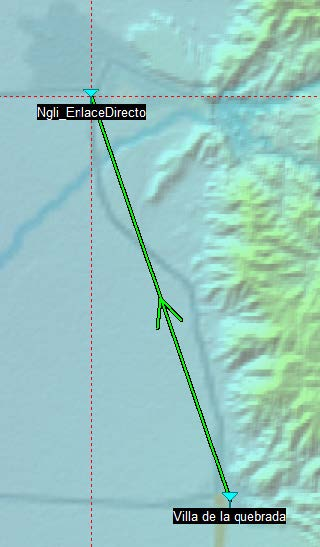
\includegraphics[width= 8 cm]{../figuras/red_transporte_6.jpg}
\caption{Vista satelital Enlace 2 de Radio Mobile}
\label{fig_red_transporte_6}
\end{figure}

Se plantea diseñar un enlace directo entre Villa de la Quebrada y Nogolí ya que la distancia entre puntos de enlace es de 11 km aproximadamente, lo que representa un enlace relativamente corto. Así mismo, el terreno presenta elevaciones que interfieren en la línea de vista entre las antenas si las torres son de un tamaño reducido; en consecuencia, se deben instalar o alquilar torres de una altura considerable (en comparación con el enlace 1). Se destaca que se ha decidido ubicar la torre en Nogolí en la posición antes mencionada ya que se encuentra en el ingreso de la localidad y se dispone de un tendido eléctrico para alimentación de los equipos.

En un diseño preliminar se plantea una modulación 2048-QAM (ver tabla \ref{tab_caracteristicas_cambium}) con una torre en Nogolí de 27 metros de altura y una en Villa de la Quebrada de 12 metros de altura. En ambas torres se utiliza una antena de 1 metro de diámetro y 35.3 dBi de ganancia obteniendo un enlace viable con el 90\% de la primer zona de Fresnel despejada y un Rx relativo de 14.6 dB Fig. \ref{fig_red_transporte_7}. Se destaca que el último parámetro mencionado tiene un valor relativamente bajo por lo que una modificación en el medio puede llegar a afectar la viabilidad del enlace (tener en cuenta que un árbol puede llegar a disminuir 3 dB el Rx relativo), por este motivo se plantean cambios en el diseño para aumentar este parámetro y lograr un enlace más robusto.

\begin{figure} [H]
\centering
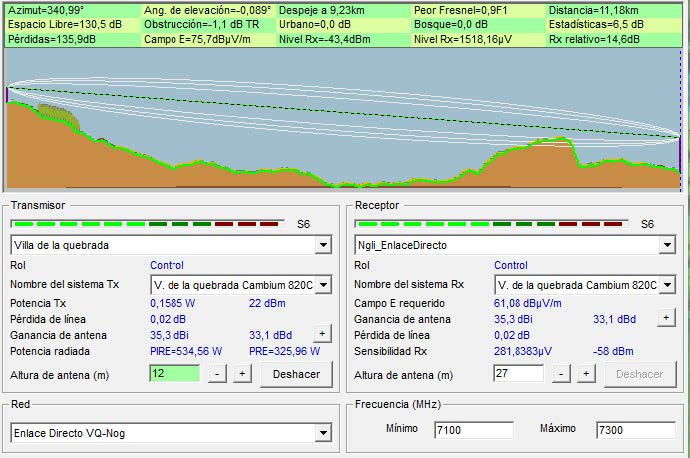
\includegraphics[width= 12 cm]{../figuras/red_transporte_7.jpg}
\caption{Configuración de equipos de Enlace 2 en Radio Mobile}
\label{fig_red_transporte_7}
\end{figure}

Ya que variando las alturas de las antenas no es posible aumentar el Rx relativo de forma considerable, las opciones son cambiar la antena por una cuyo diámetro sea mayor (aumentar la ganancia) o disminuir la modulación (aumentar la potencia Tx y disminuir la sensibilidad Rx). Se opta por la segunda opción utilizando 1024-QAM, ya que la tasa disminuye 20 Mbps aproximadamente (ver tabla equipos) y no representa una desventaja considerable teniendo en cuenta las proyecciones y la tasa máxima que se ha planificado. De este modo, se obtiene un Rx relativo de 20.1 dB con una PIRE igual a 847.23 W (ver Fig. \ref{fig_red_transporte_8}); el enlace es viable y el Rx relativo es aceptable por lo tanto se podría implementar el enlace propuesto. 

Como se tiene un valor elevado de potencia y, si bien la regulación para la frecuencia de 7 Ghz no es estricta en el sentido de la potencia radiada, pueden presentarse inconvenientes al encontrarse ubicado en una zona poblada.


\begin{figure} [H]
\centering
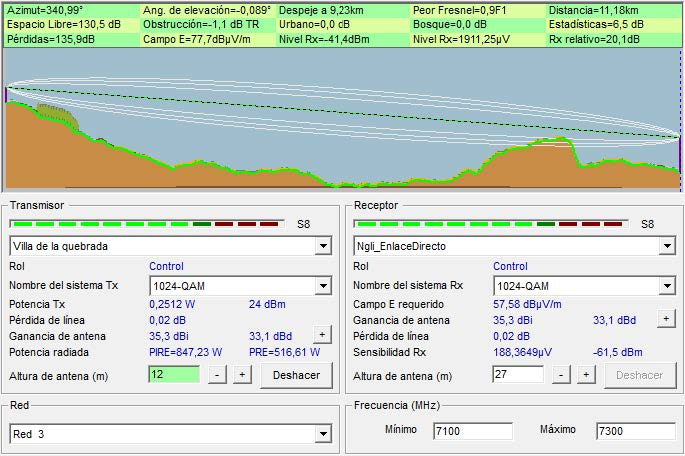
\includegraphics[width= 12 cm]{../figuras/red_transporte_8.jpg}
\caption{Alternativa de configuración de equipos de Enlace 2 en Radio Mobile}
\label{fig_red_transporte_8}
\end{figure}

\noindent\textbf{Enlace 3.a:} Villa de la Quebrada (33.018155 S.; 66.289680 O.) y Ruta 146/Repetidor 2 (32.96969 S.; 66.37423 O.)

\begin{figure} [H]
\centering
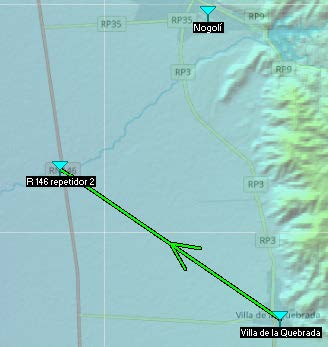
\includegraphics[width= 8 cm]{../figuras/red_transporte_9.jpg}
\caption{Vista satelital Enlace 3.a de Radio Mobile}
\label{fig_red_transporte_9}
\end{figure}

Como tercer caso, se plantea diseñar un enlace similar al “Enlace 1”, un punto medio entre Villa de la Quebrada y Nogolí por la misma Ruta 146, tal como puede observarse en la Fig. \ref{fig_red_transporte_9}.
Se utiliza una antena con una ganancia de 35,3dBi para ambos terminales, y con una sensibilidad en el receptor de -61,5dBm.

En la Fig. \ref{fig_red_transporte_10} se puede ver que las alturas de las antenas están al mismo nivel que en el enlace 1, esto es para poder hacer una comparación directa en igualdad de condiciones entre ambos enlaces. El Rx relativo obtenido en este tramo del enlace es de 26,1 dB, 4dB más que el logrado en el tramo del enlace 1.a, con un 90\% de la primer zona de Fresnel liberada. A simple vista, con estos resultados preliminares este enlace parece ser el más indicado en comparación a los enlaces anteriores, pero más adelante se verá que, al analizar el segundo tramo del enlace, se observa que disminuye su rendimiento en comparación con el enlace 1.b.

\begin{figure} [H]
\centering
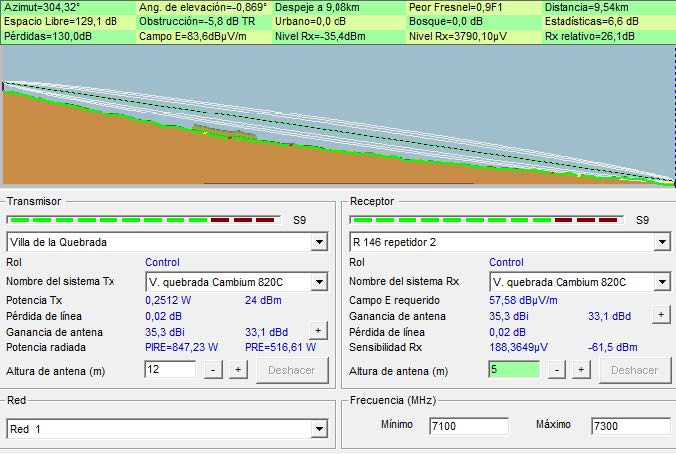
\includegraphics[width= 12 cm]{../figuras/red_transporte_10.jpg}
\caption{Configuración de equipos de Enlace 3.a en Radio Mobile}
\label{fig_red_transporte_10}
\end{figure}

\noindent\textbf{Enlace 3.b:} Ruta 146/ Repetidor 2 (32.96969 S.; 66.37423 O.) y Nogolí (32.923012 S.; 66.328737 O.)

\begin{figure} [H]
\centering
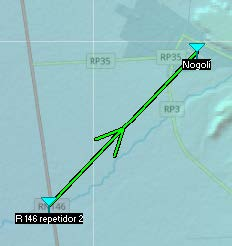
\includegraphics[width= 8 cm]{../figuras/red_transporte_11.jpg}
\caption{Vista satelital Enlace 3.b de Radio Mobile}
\label{fig_red_transporte_11}
\end{figure}

En este tramo, se vuelven a disminuir el diámetro de las antenas a 0.6 metros para una ganancia de antena de 31.1 dBi, y se mantiene la altura de las antenas por la misma razón que en el tramo anterior, con el fin de realizar una comparación en igualdad de condiciones, entre ambos enlaces (enlace 1 y enlace 3).

En la Fig. \ref{fig_red_transporte_12}, se observa que el Rx relativo es de -11.6 dB, es decir, el enlace no es viable.

\begin{figure} [H]
\centering
\includegraphics[width= 12 cm]{../figuras/red_transporte_12.jpg}
\caption{Configuración de equipos de Enlace 3.b en Radio Mobile}
\label{fig_red_transporte_12}
\end{figure}

Si se aumenta el diámetro de las antenas a 1 metro de modo que la ganancia también aumente, sigue siendo desfavorable, ya que, aunque el enlace pueda funcionar, el Rx relativo es muy bajo.

Una posible solución, para lograr un enlace viable, sería aumentar la altura de la torre en Nogolí. En la Fig. \ref{fig_red_transporte_13} se puede observar que con una torre de 10 m (dos veces más que en el primer modelo), el enlace pasa a ser viable, pero con un Rx relativo de 10,1dB, lo cual es la mitad que el obtenido en el enlace 1b.

\begin{figure} [H]
\centering
\includegraphics[width= 12 cm]{../figuras/red_transporte_13.jpg}
\caption{Alternativa configuración de equipos de Enlace 3.a en Radio Mobile}
\label{fig_red_transporte_13}
\end{figure}

Por lo tanto, analizando los tres enlaces propuestos, se llega a la conclusión de que el enlace 1 es el más viable para llevar a cabo el radio enlace, entre las localidades de Nogolí y Villa de la Quebrada. No solo por funcionalidad, sino también por la corta distancia del repetidor a la localidad de Nogolí para su mantenimiento.






\chapter{Comparativa de equipos Radio Base} \label{ane_comp_equipos_Radio_red_acceso}
\begin{large}
\noindent \textbf{Aruba 175 Series}
\end{large}
 

\medskip

La presente estación base, fabricada por Aruba Networks, cumple con el estándar 802.11 n y ofrece 2x2 MIMO logrando una tasa máxima de 300 Mbps con modulación MCS15 (64-QAM) y con una canalización de 40 
MHz (HT-40), limitando la potencia de transmisión a 17 dBm y la sensibilidad de recepción a -75 dBm. 

\begin{itemize}
\item \textbf{Dimensiones}
	\begin{itemize}
	\item[$\bullet$] 225 mm x 225 mm x 105 mm
	\item[$\bullet$] 3.5 kg
	\end{itemize}
	
\item \textbf{Ambiental}
	\begin{itemize}
	\item[$\bullet$] Temperatura de operación: -30ºC a 60ºC
	\item[$\bullet$] Humedad de operación: 5\% a 95\% no-condensada
	\end{itemize}
\end{itemize}

Se destaca que el fabricante no indica el consumo del equipo en su respectiva hoja de datos.

\medskip 

\begin{large}
\noindent \textbf{Rocket M2 Titanium}
\end{large}

cumple con el estándar 802.11 n y ofrece 2x2 MIMO con protocolo airMAX\textsuperscript \textregistered \thinspace logrando una tasa máxima de 300 Mbps con modulación MCS15 (64-QAM) y con una canalización de 40 MHz, limitando la potencia de transmisión a 22 dBm y la sensibilidad de recepción a -75 dBm. Así mismo, Ubiquiti Networks, Inc. ofrece software como airOS\textsuperscript \textregistered \thinspace , airVIEW\textsuperscript \textregistered \thinspace  y airCONTROL\textsuperscript \textregistered \thinspace destinados al mantenimiento e instalación del dispositivo, así como mantenimiento de la red.


\begin{itemize}
\item \textbf{Dimensiones}
	\begin{itemize}
	\item[$\bullet$] 160 mm x 80 mm x 44 mm
	\item[$\bullet$] 350 g
	\end{itemize}
	
\item \textbf{Ambiental}
	\begin{itemize}
	\item[$\bullet$] Temperatura de operación: -30ºC a 75ºC
	\item[$\bullet$] Humedad de operación: 5\% a 95\% condensada
	\end{itemize}
\end{itemize}

El fabricante indica el consumo máximo (6.5 W) del equipo, dato importante a la hora de realizar cálculos de consumo de energía.

\medskip

Se observa que la estación base de Ubiquiti Networks Inc. presenta mayor potencia de transmisión a la misma modulación, así como un paquete de software de análisis que facilita el mantenimiento del equipo. Por tal motivo, se decide la utilización del equipo \textbf{Rocket M2 Titanium}.







\chapter{Comparativa equipos GPON} \label{ane_comp_equipos_gpon_acceso}

Para comenzar, se mencionan las características más relevantes de la OLT
y ONT de marca Furukawa.\bigskip

\textbf{OLT: Furukawa GPON FK-OLT-G4S}\medskip
\begin{itemize}
\item Hasta 128 ONTs por interface GPON.
\item Velocidad de 2.5 Gbps en downstream. (De OLT a ONT).
\item Velocidad de 1.25 Gbps en upstream. (De ONT a OLT).
\item Longitud de onda de transmisión: 1490 nm.
\item Longitud de onda de recepción: 1310 nm.
\item Potencia óptica de transmisión: 1.5 dBm $\backsim$ +5 dBm.
\item Potencia óptica de recepción (sensibilidad); -8 dbm $\backsim$ -28 dBm.
\item Soporta ITU-T G.984.4 para gestión y control de la interface de la ONT.
\item 20 km de rango de transmisión (60 km de alcance lógico).
\item ONT recomendada por el fabricante: FK-ONT-G400B/PoE S2.
\end{itemize} \bigskip

\textbf{ONT: Furukawa FK-ONT-G400B/PoE S2}\medskip
\begin{itemize}
\item 1 puerto óptico SC/APC.
\item Velocidad de 2.5 Gbps en downstream (de OLT a ONT).
\item Velocidad de 1.25 Gbps en upstream (de ONT a OLT).
\item Potencia óptica de transmisión: 0,5 dBm $\backsim$ 5 dBm
\item Potencia óptica de recepción (Sensibilidad): -28 dBm.
\item Longitud de onda de Upstream: 1310 nm.
\item Longitud de onda de Downstream: 1490 nm.
\item ONT compatible con el estándar ITU-T G.984.
\end{itemize}\bigskip

Luego, se sigue por mencionar los equipos pre-seleccionados de la marca Ubiquiti Networks Inc..\bigskip

\textbf{OLT: Ubiquiti UF-OLT}\medskip
\begin{itemize}
\item Hasta 128 ONTs por interface GPON.
\item Velocidad de 2.5 Gbps en upstream (De OLT a ONT).
\item Velocidad de 1.25 Gbps en downstream (De ONT a OLT).
\item Longitud de onda de transmisión: 1490 nm.
\item Longitud de onda de recepción: 1310 nm.
\item 8 puertos GPON SFP, para servicio hasta 128 ONTs/puerto, con un
total de hasta 1024 ONTs por OLT.
\item Soporta ITU-T G.984.4 para gestión y control de la interface de la
ONT.
\item 20 km de rango de transmisión (60 km de alcance lógico).
\item ONT recomendada por el fabricante: FK-ONT-G400B/PoE S2.
\end{itemize}\bigskip

Los puertos GPON de la OLT UFiber han sido diseñados para ser usados
con dos tipos de módulos que solo varían en la potencia de recepción y la
sensibilidad del receptor. Dichos módulos se mencionan a continuación:\bigskip

\begin{itemize}\medskip
\item[$\bullet$] \textbf{FiberModule UF-GP-B+}:
	\begin{itemize}
	\item[$\circ$] Tipo de conector: SC/UPC.
	\item[$\circ$] Potencia de transmisor: 1.5 ~ 5 dBm.
	\item[$\circ$] Potencia de recepción (sensibilidad): -28 ~ -8 dBm.
	\item[$\circ$] Fibra mono-modo.
	\end{itemize}
\item[$\bullet$]\textbf{FiberModule UF-GP-C+}:
	\begin{itemize}
	\item[$\circ$] Tipo de conector: SC/UPC.
	\item[$\circ$] Potencia de transmisor: 3 $\backsim$ 7 dBm.
	\item[$\circ$] Potencia de recepción (sensibilidad): -30 $\backsim$ -12 dBm.
	\item[$\circ$] Fibra mono-modo.
	\end{itemize}
\end{itemize}\bigskip

Como puede notarse en la comparación de características de los módulos,
el UF-GP-C+ tiene mejores prestaciones, aunque su costo es mayor, por lo
cual en los siguientes cálculos se demostrará si es necesario o no hacer un
gasto extra.\bigskip

\textbf{ONT: UFiber Nano G} \medskip
\begin{itemize}
	\item 1 puerto óptico SC/APC.
	\item Velocidad de 2.5 Gbps en downstream (de OLT a ONT)
	\item Velocidad de 1.25 Gbps en upstream (de ONT a OLT).
	\item Potencia óptica de transmisión (Clase B+): 1,5 dBm $\backsim$ 5 dBm.
	\item Potencia óptica de recepción (Sensibilidad): -28 dBm $\backsim$ -8
dBm.
	\item Longitud de onda de Upstream: 1310 nm.
	\item Longitud de onda de Downstream: 1490 nm.
	\item ONT compatible con el estándar ITU-T G.984.
\end{itemize} \bigskip

Por último, siguiendo las recomendaciones del Ing. Recondo Jorge, jefe de redes de la empresa prestadora de servicios BVC (Bahía Visión Color), se analiza el OLT de marca Fiberhome y ONT de marca Huawei.\bigskip

\textbf{OLT: Fiberhome AN5516-04S}\medskip
\begin{itemize}
\item 4/8 interfaces GPON clase B+.
\item Hasta 1024 ONTs (con dos niveles de splitter de 1:32).
\item Velocidad de 2.488 Gbps en downstream. (De OLT a ONT).
\item Velocidad de 1.244 Gbps en upstream. (De ONT a OLT).
\item Longitud de onda de transmisión: 1490/1550 nm.
\item Longitud de onda de recepción: 1310 nm.
\item Potencia óptica de transmisión: 1.5 dBm $\backsim$ +5 dBm.
\item Potencia óptica de recepción (sensibilidad); -8 dbm $\backsim$ -28 dBm.
\item Soporta fibra mono-modo ITU-T G.652 y G.657 con conectores SC/PC.
\item 20 km de rango de transmisión (60 km de alcance lógico).
\end{itemize}\bigskip

\textbf{ONT: Huawei HG8245u}\medskip
\begin{itemize}
\item Interface GPON clase B+, Ethernet, POTS y USB2.0.
\item soporta IEEE 802.11 b/g/n (2.4 GHz) e IEEE 802.11 a/n/ac (5GHz).
\item 2x2 MIMO (2.4 GHz) 3x3 MIMO (5 GHz).
\item Ganancia de antena 2 dBi.
\item 300 Mbps en 2.4 GHz y 1300 Mbps en 5 GHz.
\item Longitud de onda de transmisión: 1310 nm.
\item Longitud de onda de recepción: 1490 nm.
\item Potencia óptica de transmisión: 0.5 dBm $\backsim$ +5 dBm.
\item Potencia óptica de recepción (sensibilidad); -8 $\backsim$ -27 dBm.
\item Implementa FEC Bidireccional. \footnote{FEC: Fordward Error Correction.}
\end{itemize}\bigskip









\chapter{Simulación con programa WinProp} \label{ane_simulacion_Radio_red_acceso}

Se decide colocar los APs a 8m de altura (alumbrado público) y las
NanoStation de cada usuario a 3 m de altura (en el techo de la vivienda).

\medskip

En primer lugar se genera el plano de la localidad de Nogolí con la ayuda del programa WallMan, donde las alturas de las edificaciones y vegetación se consideran en promedio de la
siguiente manera:

\begin{itemize}
\item Casa promedio: 3 metros
\item Galpones o edificios de más de 200 m\textsuperscript 2: 5 metros
\item Arboleda: 4.5 metros
\item Galpones pequeños: 4.5 metros
\end{itemize}

En Fig. \ref{Fig_UbicacionDeAPs} se expone la ubicación de los APs.

\begin{figure} [H]
\centering
\includegraphics[width= 15cm]{../figuras/ubicacionDeAPs_Acceso.JPG}

\caption{Ubicación de APs. Programa ProMan}
\label{Fig_UbicacionDeAPs}
\end{figure}


Luego se prosigue a realizar la simulación con el programa ProMan, de esta manera se puede estimar la viabilidad de los enlaces teniendo en cuenta la región y las fuentes de interferencia allí presentes. \medskip

A continuación se exponen las capturas de la simulación realizada para cada AP, donde se ha definido una altura de 3 m para las NanoStation (la simulación se realiza a 3 m). Además, se define una  potencia de transmisión de cada AP en 22 dBm ya que de esta manera se obtiene una PIRE\footnote{Potencia Isotrópica Radiada Efectiva} de 35 dBm (la
ganancia de la antena es de 13 dBi). La normativa vigente\footnote{Resolución
127/12, Boletín Oficial 32.578, 07/02/13, Comisión Nacional de Comunicaciones.} impone una PIRE máxima de 36 dBm en la banda de 2.4 GHz.

\medskip

\begin{figure}[H]
\centering
\subfigure{\includegraphics[height = 6 cm]{../figuras/simul_antena1.jpg}} 
\subfigure{\includegraphics[height = 6 cm]{../figuras/referencia_simul_antena1.jpg}}
\caption{Simulación AP 1, Downlink}
\label{fig_SimulAP1_acceso}
\end{figure}

\medskip

\begin{figure}[H]
\centering
\subfigure{\includegraphics[height = 6 cm]{../figuras/simul_antena2.jpg}} 
\subfigure{\includegraphics[height = 6 cm]{../figuras/referencia_simul_antena2.jpg}}
\caption{Simulación AP 2, Downlink}
\label{fig_SimulAP2_acceso}
\end{figure}

\medskip

\begin{figure}[H]
\centering
\subfigure{\includegraphics[height = 6 cm]{../figuras/simul_antena3.jpg}} 
\subfigure{\includegraphics[height = 6 cm]{../figuras/referencia_simul_antena3.jpg}}
\caption{Simulación AP 3, Downlink}
\label{fig_SimulAP3_acceso}
\end{figure}

\medskip

\begin{figure}[H]
\centering
\subfigure{\includegraphics[height = 6 cm]{../figuras/simul_antena4.jpg}} 
\subfigure{\includegraphics[height = 6 cm]{../figuras/referencia_simul_antena4.jpg}}
\caption{Simulación AP 4, Downlink}
\label{fig_SimulAP4_acceso}
\end{figure}

\medskip

\begin{figure}[H]
\centering
\subfigure{\includegraphics[height = 6 cm]{../figuras/simul_antena5.jpg}} 
\subfigure{\includegraphics[height = 6 cm]{../figuras/referencia_simul_antena5.jpg}}
\caption{Simulación AP 5, Downlink}
\label{fig_SimulAP5_acceso}
\end{figure}

\medskip

Se puede observar que cada AP brinda cobertura a su zona asignada y a parte de otras zonas (recordar que la sensibilidad en el abonado es de -75 dBm). 

\medskip

Se ha realizado la simulación de la conexión con enfoque en la sensibilidad de la NanoStation Loco, concluyendo que es posible la conexión en las 5 zonas. Se destaca que la potencia de transmisión de la NanoStation es menor que la de la estación base (17 dBm) por lo que se debe realizar la simulación para determinar la viabilidad de las conexiones. \medskip

Se posicionan las NanoStation a 3 m de altura (en el programa ProMan), en las viviendas más alejadas a las estaciones base pertenecientes a cada zona. En Fig. \ref{fig_Ubicacion_Nano} se expone la disposición de las mismas.\medskip

\begin{figure} [H]
\centering
\includegraphics[width= 15cm]{../figuras/Ubicacion_NSLoco.JPG}

\caption{Ubicación de NanoSations Loco M2, simulación Uplink. ProMan.}
\label{fig_Ubicacion_Nano}
\end{figure}

A continuación se exponen los resultados de las simulaciones.

\begin{figure}[H]
\centering
\subfigure{\includegraphics[height = 6 cm]{../figuras/simul_NSLoco_1.jpg}} 
\subfigure{\includegraphics[height = 6 cm]{../figuras/referencia_simul_NSLoco_1.jpg}}
\caption{Simulación NS Loco Zona 1, Uplink}
\label{fig_SimulLoco1_acceso}
\end{figure}



\begin{figure}[H]
\centering
\subfigure{\includegraphics[height = 6 cm]{../figuras/simul_NSLoco_2.jpg}} 
\subfigure{\includegraphics[height = 6 cm]{../figuras/referencia_simul_NSLoco_2.jpg}}
\caption{Simulación NS Loco Zona 2, Uplink}
\label{fig_SimulLoco2_acceso}
\end{figure}



\begin{figure}[H]
\centering
\subfigure{\includegraphics[height = 6 cm]{../figuras/simul_NSLoco_3.jpg}} 
\subfigure{\includegraphics[height = 6 cm]{../figuras/referencia_simul_NSLoco_3.jpg}}
\caption{Simulación NS Loco Zona 3, Uplink}
\label{fig_SimulLoco3_acceso}
\end{figure}


\begin{figure}[H]
\centering
\subfigure{\includegraphics[height = 6 cm]{../figuras/simul_NSLoco_4.jpg}} 
\subfigure{\includegraphics[height = 6 cm]{../figuras/referencia_simul_NSLoco_4.jpg}}
\caption{Simulación NS Loco Zona 4, Uplink}
\label{fig_SimulLoco4_acceso}
\end{figure}



\begin{figure}[H]
\centering
\subfigure{\includegraphics[height = 6 cm]{../figuras/simul_NSLoco_5.jpg}} 
\subfigure{\includegraphics[height = 6 cm]{../figuras/referencia_simul_NSLoco_5.jpg}}
\caption{Simulación NS Loco Zona 5, Uplink}
\label{fig_SimulLoco5_acceso}
\end{figure}



\begin{figure}[H]
\centering
\subfigure{\includegraphics[height = 6 cm]{../figuras/simul_NSLoco_6.jpg}} 
\subfigure{\includegraphics[height = 6 cm]{../figuras/referencia_simul_NSLoco_6.jpg}}
\caption{Simulación NS Loco Zona 6, Uplink}
\label{fig_SimulLoco6_acceso}
\end{figure}

Se observa que es viable la ubicación de los equipos, ya que al colocar las NanoSation al límite de cada zona es posible la comunicación de forma bidireccional. \footnote{ La NanoStation envía datos la estación base y viceversa.} \medskip

























\end{document}
